\documentclass{uathesis}
% v0.1
%  20/06/2013 - first draft of chapters
%  
%
\usepackage[pdftex]{graphicx}
\usepackage{mathptmx} % Use the Adobe Times Roman as the default text font together with math symbols from the Symbol, Chancery and Computer Modern fonts

\usepackage{xcolor} % Required for specifying colors by name
\definecolor{ocre}{RGB}{52,177,201} % Define the orange color used for highlighting throughout the book

\usepackage{microtype} % Slightly tweak font spacing for aesthetics
\usepackage[utf8]{inputenc} % Required for including letters with accents
\usepackage[T1]{fontenc} % Use 8-bit encoding that has 256 glyphs
\usepackage{listings}
%\usepackage[backend=bibtex,style=verbose-trad2]{biblatex}

% \usepackage[style=alphabetic,sorting=nyt,sortcites=true,autopunct=true,babel=hyphen,hyperref=true,abbreviate=false,backref=true,backend=biber]{biblatex}
%\addbibresource{bibliography.bib} 
% BibTeX bibliography file
% \defbibheading{bibempty}{}
%usepackage to attach appendices
\usepackage[toc,page]{appendix}
%\usepackage{minted}
\usepackage{rotating}
\usepackage[colorinlistoftodos]{todonotes}
\usepackage{algorithm,
						algpseudocode,
            amsfonts,
            amsmath,
            amssymb,
            amsthm,
						adjustbox,
						blindtext,
						calc,
						color, 
						colortbl,
						epstopdf,
						fancyhdr,
						float,
						longtable,
						lastpage,
						latexsym,
						listings,
						multirow,
						makeidx,
						pbox,
						pseudocode,
						placeins,
						setspace,
						subcaption,
						%tabularx,
						titlesec,
            url,
            varwidth,
            wrapfig,
						xspace
            }
\usepackage[belowskip=-15pt,aboveskip=0pt]{caption}
\DeclareMathOperator\erf{erf}
\setlength{\intextsep}{10pt plus 2pt minus 2pt}
\setlength{\headheight}{15pt}
\setlength{\footskip}{10pt}
\parskip1.5mm
\newlength{\temptextwidth}
\newenvironment{abstract}{
\begin{flushright}
\begin{minipage}[t]{0.7\textwidth}
\it
}{
\end{minipage}
\end{flushright}
\hskip5mm
}

\theoremstyle{definition}
\newtheorem{example}{Example}[section]
\DeclareGraphicsExtensions{.pdf,.jpeg,.png,.PNG}
\usepackage[font=small]{caption}
\setcounter{secnumdepth}{3}
\pagestyle{fancy}
\fancyhf{}
\rfoot{\small \textbf{Page \thepage \hspace{1pt} of \pageref{LastPage}}}
\lhead{Chapter\ \thechapter:\rightmark}
\newcommand{\defaultspacing}{\onehalfspacing}
%\onehalfspacing
\setlength{\parskip}{0.4cm}%

%Remove header from first page of each Chapter
\makeatletter
\renewcommand\chapter{\if@openright\cleardoublepage\else\clearpage\fi
                    \thispagestyle{empty}% original style: plain
                    \global\@topnum\z@
                    \@afterindentfalse
                    \secdef\@chapter\@schapter}
\makeatother
\titleformat{\chapter}
{\normalfont\bfseries}{\chaptertitlename\ \thechapter:}{0.5em}{}
\makeindex
\newlength{\defaultlinespace}
\setlength{\defaultlinespace}{\baselineskip}

%includeonly{Appendix}

\begin{document}
\thispagestyle{empty}
\begin{center}
\vspace*{3cm}
{\Huge\baselineskip=1.5cm
A Non-Connection Breaking PEP for Narrowband Satellite Links}\\
\mbox{}\par % Book title
\vspace*{1cm}
{\huge Fuli Fuli}\par % Author name
\vspace{7cm}

{\Large A thesis submitted in fulfilment of the requirements
for the degree of Master of Science in Computer Science,
the University of Auckland, April 2018}
\end{center}


\chapter*{Abstract}

Internet connectivity via satellite link on small and remote Pacific Islands has historically suffered from poor performance regarding data transfers. The inherent propagation latency combined with the narrowband bottleneck nature of the link causes significantly delayed responses of the TCP congestion control algorithms that contribute to a poor Internet user experience. In more recent times, many of these problems have been mitigated through the development of more sophisticated satellites capable of carrying 1Gbps to 2Gbps feeds which would reduce the bottleneck effect considerably. Many affected islands in the Pacific, however, do not have the economic means to upgrade their satellite link and so are left with link data rates ranging from a few Mbps to a few hundred Mbps. Improvement to Internet connectivity in these places is still a work in progress. Performance Enhancing Proxies (PEP) solutions have been proposed as a way of solving this problem, but many of the commercial PEPs are costly and may not suit the low socio-economic budgetary constraints of many Pacific Island nations. Other less costly open source solutions adopt a TCP splitting/connection breaking PEP approach that violates the fundamental end to end semantics of TCP which causes its own problems. This research develops the first open source Linux based non-connection breaking PEP that is inexpensive and can be deployed easily on any computer along the link path. The PEP is coded in C using raw socket programming and has been tested on the University of Auckland's Pacific Island Satellite Simulator. The PEP in its present state already offers small goodput gains for long downloads. The current codebase is intended as a platform for further development. This thesis describes the motivation for and the development of this platform and points out the future potential for ongoing development.





%\include{Preface}
\tableofcontents
\clearpage
\mbox{}
%chapter 1: Introduction
%----------------------------------------------------------------------------------------
%	CHAPTER 1
%----------------------------------------------------------------------------------------

%\chapterimage{head2.png} % Chapter heading image


\chapter{Introduction}

Internet usage/data transfers in some of the Pacific Islands are problematically slow ~\cite{4}. Many of these islands do not have the infrastructure or budget for undersea fibre-optic cable connected Internet but rather rely on satellite link Internet ~\cite{3}. Samoa and Tonga, for instance, have only recently had these fibre-optic cables connected to the high-rate Internet but unfortunately, many of the smaller islands still rely on satellite connectivity ~\cite{3}. The result is that many Pacific Islands are left with slow, archaic Internet data rates due to the latency and bottleneck bandwidth of the satellite link. This thesis will discuss the problems this creates ~\cite{4}. This work looks at options to help solve these issues and creates the foundation for a performance enhancing proxy (PEP) that primarily aims to counteract the factors creating slow Internet data rates. In general, most PEPs give TCP senders the illusion that packets are traveling over a shorter distance and thus help solve some of the issues created by latency and the bottleneck nature of the satellite link ~\cite{6}.This thesis first discusses a variety of PEP concepts and then introduces our variation on the theme: a \emph{non-connection breaking PEP}. In this chapter, we will briefly look at the problem and motivation for our thesis. 

\section{Problem And Motivation}\label{Motivation}

\emph{The problem:} In a nutshell, TCP originated in terrestrial networks (of comparatively low latency) in all its variant forms (TCP Reno, TCP Cubic etc.) does not work well with narrowband satellite links ~\cite{5}. On satellite links, the latency between the sender and receiver is higher than on purely terrestrial links. It is up to 500 ms round trip time (RTT) or more via geostationary (GEO) satellites, 120 ms or more via medium earth orbit satellites (MEO). The further problem is that the narrowband nature of many satellite links creates a bandwidth bottleneck at which congestion can occur ~\cite{4}. This combination of latency and bottleneck is the root of the problem which this thesis will offer more in-depth explanations on later ~\cite{7}~\cite{8}. The symptoms of this problem, at least from an Internet users perspective, are evidenced by excruciatingly slow Internet speeds. For these Internet users connected solely to a satellite link, such as those living in the Pacific Islands mentioned previously, web browsing becomes frustratingly slow and large downloads, or streaming is next to impossible ~\cite{4}. The symptoms of this problem from a network perspective are the underutilisation of the link, excessive queue oscillation at the input to the satellite link, unnecessary retransmissions and false timeouts which all contribute to degraded Internet service for users ~\cite{8}~\cite{9}. (Chapter 2 will discuss these problems in more depth). The essential elements that comprise our problem stem from TCP's mechanism to guarantee reliability and TCP congestion control ~\cite{10}~\cite{11}. \\

The transport layer protocol (TCP) ensures that all data sent for applications between two hosts is delivered with reliability, integrity, in-order, and without duplication . TCP reliability means that the data delivery is reliable and guaranteed to reach the receiver and both receiver and sender are informed of successful deliver. Integrity assures that the data is not corrupted and is received with no errors ~\cite{1}. In-order says the information is delivered to the receivers application layer in the same order it was sent. Without duplication means that the receiver will not receive the same data twice ~\cite{1}~\cite{2}.\\

The TCP mechanism to guarantee reliability is achieved via acknowledgements (ACKs) from the receiver to the sender. The ACKs let the sender know that data has been successfully delivered. If the sender does not receive an ACK back for data sent within a certain timeout period, TCP makes sure the data is retransmitted until an ACK is received (reliable delivery) ~\cite{1}~\cite{12}. \\

TCP also has what is known as \emph{"slow start”}, which is part of a congestion control mechanism to prevent the sender flooding the network and overwhelming the buffer queues of intermediate routers which will lead to datagrams/packets being dropped. Slow start ensures the senders initially send out only a few packets over the network, gradually increasing the number of packets sent out dependent on the acknowledgements (ACKs) returned. The rate of growth of packets sent depends on the TCP variant being used. For TCP Reno, for instance, the growth is exponential. It will send one packet, receive an ACK and then send two, receive an ACK then send four and so forth, increasing exponentially until an ACK fails to return ~\cite{1}~\cite{12}. \\

When an ACK fails to return in the allotted timeout period, TCP initiates "exponential backoff" which halves the number of datagrams being sent. TCP will continue to halve this output until all ACKs are being returned once again. The exponential backoff is then replaced with "congestion avoidance" which will increase the sender's output linearly to avoid congestion and packet loss ~\cite{1}. The linear growth of sender output at this point, rather than exponential, is TCP's way of trying not to overshoot the maximum capacity of the network that would lead to packet loss and another "exponential backoff". The goal of these TCP mechanisms is to reach a network "sweet spot", so to speak, that allows the senders to make the maximum use of the network link available as possible without packet loss ~\cite{1}~\cite{12}. With terrestrial-based communications between terrestrial senders and receivers, these TCP mechanisms work well and mainly achieve that goal. \\

TCP encounters many problems, however, when traversing via a narrowband satellite link. Firstly, the satellite link is a natural bottleneck because most terrestrial applications run on Internet speeds of 1GB to 2GB per second feeding into a satellite link that has a 16Mb per second connection speed ~\cite{4}~\cite{5}. This factor exacerbates one of the original problems TCP is designed to mitigate. That problem being the intermediate router buffers being filled up too quickly by the sender output, as we now have a situation analogous to having a water funnel designed to allow a flow of 160ml per second trying to cope with a bucket of water being poured into it at 2 Litres per second. Overflow is inevitable, and it will happen much sooner than if it were a TCP communication between senders/receivers on land ~\cite{8}~\cite{10}. \\

The bottleneck problem mentioned above leads us to the other related major issue TCP encounters with satellite links; namely the latency it must contend with (typically around 500ms round trip time). When the terrestrial sender's packet rate quickly exceeds the satellite link’s transmission rate, packets are put in a queue. Eventually, the queue may overflow, losing packets which will mean the sender does not receive the corresponding ACK, and the sender will need to retransmit the packet ~\cite{11}~\cite{13}. The added problem that the link latency causes here is that even packets that get through to the receiver may end up being retransmitted because of the ACKs timeout when they take too long to get back to the sender. Therefore, the satellite link presents an overly exaggerated account of packet loss to the sender causing issues that would not be present in terrestrial TCP environments ~\cite{13}.\\

The sender believes the packets have been lost and retransmits. These false timeouts and subsequent retransmissions trigger "exponential backoff" needlessly. (The satellite link is also prone to random link losses unrelated to congestion which also trigger "exponential backoff" unnecessarily and contribute to the overall inefficient use of the network, but this will be discussed later in the thesis) ~\cite{13}~\cite{14}. At any one time, the satellite link carries multiple simultaneous TCP connections, so all the senders exponentially back off simultaneously.  The queues are then given a chance to clear as the senders drastically reduce output, but they sit idle for longer than desired as the senders cease emitting over the link. This simultaneous backoff as a result of false timeouts caused by latency is a serious contributing factor to one of the significant issues previously mentioned with the TCP over satellite link communication; namely the underutilisation of the link ~\cite{13}.\\


At the same time, all the delayed ACKs that the sender regarded as lost (false timeouts and retransmissions) arrive back at the senders at more or less the same time. This heavy bombardment of ACKs causes the senders to ramp up again simultaneously, and via slow start, all rapidly increase their packet output over the large latency narrowband satellite bottleneck link which floods the buffer queues causing another cycle of congestion resulting in false timeouts and retransmissions and the subsequent excessive exponential backoff. The perpetuation of a TCP cycle of backing off and ramping up once again is established and fixed in place. This effect is called \emph{queue oscillation} which is quite reasonable in networks to an extent ~\cite{4}~\cite{5}. Provided the queue oscillation occurs only occasionally and relatively slowly, resulting in minimal packet loss, then it is an acceptable state to be in. The queue never overflows or empties for very long. However, due to the exaggerated account of packet loss triggered by the issues as mentioned earlier with TCP over satellite links, the result is \emph{extreme queue oscillation} which is undesirable. The satellite link switches between extreme states of idleness and link underutilisation and extreme state of network flooding senders resulting in significant packet loss ~\cite{4}~\cite{5}.\\


Ideally, we want our senders to receive ACKs for delivered data faster to eliminate false timeouts and retransmissions or cut them significantly. If the sender could be informed of delivered packets sooner, it would help ease queue overflow and reduce the extremity of the queue oscillation caused by the issues mentioned earlier. This problem has been a topic of research for decades ~\cite{16}. One of the solutions, which this thesis will revolve around, is a Performance Enhancing Proxy (PEP) that can sit between the client and the server-side of the satellite link ~\cite{6}. There are many variations of PEP's proposed over the years, but the one considered as most useful by many is the connection breaking PEP (a.k.a, TCP splitting PEP) ~\cite{14}. To the server, the PEP will seem to be the client. Likewise, to the client, the PEP will appear to be the server ~\cite{6}. The PEP will receive the packets and send an ACK to tell the sender that client has received the data (or vice versa). The PEP will then pass the data in a \emph{separate connection} to the client pretending to be the sender. This reduces the latency on each of the two connections and lessens the effects of queue oscillation, but breaks the fundamental end-to-end principle of the Internet. This breaking of the principle is problematic in itself and will be detailed further in this thesis~\cite{6}. \\

\emph{The motivation:} This research could be of value to specific regions in the Pacific where inhabitants rely on satellite link Internet (e.g., Niue, Cook Islands, Tuvalu, Kiribati, …) ~\cite{3}~\cite{4}. NZ, for instance, is investing heavily in bringing speedier broadband services via fibre optics over the next few years. Pacific islands are being left far behind the world, and this is one motivation for this project from the authors point of view. It is also an topic that can be applied to other areas where the performance of TCP protocols can suffer degradation such as satellite link connectivity to ships and planes ~\cite{4}.

\section{Research Objectives/Questions}\label{Objective}
The Research Objectives/Questions are as follows:\\

The research will contribute to the already existing field of study on Performance Enhancement Proxies (PEP). Many different types of PEP have been developed to enhance the poor performance of Internet protocols caused by specific characteristics of a link or subnetwork on the path ~\cite{6}. This thesis will focus only on satellite link PEPs and aims to develop an alternative to two existing open source solutions called TCPEP and PEPsal. These PEP solutions essentially create two distinct connections between the PEP, the server and the PEP and client and are therefore connection breaking ~\cite{6}. The solutions use conventional TCP socket protocols. This breakage of the fundamental end to end principle of the Internet is a problem ~\cite{13}~\cite{14}, and this thesis will develop a platform that avoids the connection breakage. \\

\section{Proposed Solution}\label{Solution}
This research aims to create a non-connection breaking performance-enhancing proxy. I will be using raw sockets, so I can customise the protocols to suit our view of the network. For example, we can eventually modify the ACK advertised window to be smaller if we think we sent enough packets to control the flow more effectively. We can create copies of the data packets received in a cache and send an ACK immediately, even if we have not received an ACK back from the real receiver yet. When the real ACK arrives, we can delete the copy. If the real ACK does not arrive, we can resend the data packet copy from cache.\\

We have an advantage over the other PEP solutions using conventional TCP protocols because we will be able to program flow control with knowledge that the client and server may not have. For instance, with Pacific Island scenarios with a very small local latency, so we will know the approximate Round Trip Time (RTT) from the PEP to the clients. Hence we can manipulate flow control accordingly for maximum efficiency ~\cite{4}.

\subsection{Novelty}\label{Novelty} 
Most, if not all, PEPs that are not proprietary or commercial are connection breaking PEPs (TCP splitting) ~\cite{6}. This means the PEP sits in the middle of two connections and acts as a proxy mimicking the side that client/sender thinks they are directly communicating to and this can cause problems ~\cite{6}. For instance, if one server goes down, but the client has sent data to the server and received confirmation from the PEP (via a PEP generated ACK) that the server has received the data, this client will falsely believe the data has been delivered. The solution presented in this thesis differs from these PEPs because it will not break the connection between either side ~\cite{6}. 
%------------------------------------------------

\section{Thesis Structure}\label{Structure}
This section will give a breakdown of the thesis structure; In chapter one, we have examined the motivation and problems for this research on Performance Enhancing Proxies(PEP). Research objectives have been outlined, and the proposed solution to the problem has been explained briefly. \\

Chapter 2, this thesis will provide the reader with some background to give context. The section will provide a synopsis of the TCP/IP protocol suite and will then cover TCP traffic control methods starting with a brief overview of TCP flow control and ending with the TCP congestion control/Slow Start which is the more pertinent of the two control methods for this thesis. The thesis will also go into more detail about the Internet problems in Pacific Islands. Finally, this chapter will conclude with a summary of "Other concepts used in this thesis" which will provide references to many topics relating to the thesis that the reader may choose to conduct further research on..  \\

Chapter 3 will begin by defining a performance enhancing proxy before delving into a literature review to give a history brief of the satellite link issues and types of solutions that have been tried and tested in the past, including the variety of PEPs. Next, the chapter will look at the different PEP categorisations and explain where our PEP fits. Finally, this chapter will look at past implementations of PEPs in existence now, how they are categorised in comparison to our PEP and compare and contrast. \\ 

Chapter 4 is about the methodology we use in creating and experimenting with the PEP. It will cover a specific type of socket programming (RAW SOCKET) how it differentiates from socket programming as well as how it is essential for our proposed solution. It will show the steps I have taken to create the PEP and how a non-connection breaking PEP applies to the Pacific Island network infrastructure. It will guide the reader through the steps of creating a packet sniffer, a packet injector and then through the creation of an ARP table and ARP requests packets for forwarding packets. Finally, the reader will be given a rundown of our proposed non-connection breaking PEP and taken through a step by step walkthrough of the PEP logic (i.e.the actions the PEP takes as it encounters incoming packets) followed by the implementation of that logic and reasoning for it.\\

Chapter 5 looks at our findings, will give a detailed description of the University of Auckland's Pacific Island Satellite Simulator testbed. This chapter discusses the overall project findings and it will be using the PEP on the University of Auckland Pacific Island satellite simulator and testing these results against PEPsal experiments also used on this testbed.\\

Finally, Chapter 6 concludes the thesis by giving an overall research summary and discussing its practical implications. We analyse the results, strengths and weaknesses/limitations of my research and end with suggestions for further research avenues that could be explored to improve the PEP.


%chapter 2: Literature Review
%----------------------------------------------------------------------------------------
%	CHAPTER 2
%----------------------------------------------------------------------------------------

\chapter{Background}\label{Background}

This chapter will provide the reader with background knowledge on fundamental concepts in this thesis.\\

This chapter will identify and discuss the main problem with narrowband satellite link performance in more detail. Section 2.1 briefly describes the TCP protocol. Section 2.1.1 defines an Internet protocol. Section 2.1.2 takes an in-depth look at the TCP/IP protocol which is the predominant protocol used on the Internet today. Section 2.2 looks at the TCP traffic control methods which are key factors in our satellite link problem. Section 2.2.1 starts with a traffic control method as utilised from the receivers side. This TCP traffic control method is known as \emph{TCP flow control} and is key to understanding the \emph{future work} section. Section 2.2.2 presents the TCP traffic control method as utilised from the sender's side. This method is called \emph{TCP congestion control}, and this section will examine a specific component of this traffic control method most pertinent to the PEP in this thesis known as \emph{slow start}. Section 2.2.3 looks at congestion control in the satellite link environment and explains why slow start does not efficiently operate here and in fact, compounds and contributes to the problem. Section 2.2.4 takes a look at Pacific Island Internet data rates today and finally Section 2.2.5 looks at other concepts used in this thesis and provides links and references to these topics.

\section{TCP- Transmission Control Protocol}\label{TCP}
Since even before the inception of the Internet, many methods/processes and protocols have been devised to enable smooth communication between computers.  TCP/IP emerged as the fundamental communication suite in Internet communication today ~\cite{1}~\cite{2}.\\

\subsection{What is an internet protocol?}
A protocol establishes the rules of engagement between two communicating entities on the Internet. Much like humans have our protocols for proper communication to one another (e.g., taking turns speaking and listening, not talking over one another), computer networks have contracts/rules of engagement that are for the establishment of smooth communication. Many protocols have emerged since the Internet was born, but TCP/IP has become the dominant one used today ~\cite{1}~\cite{2}.

\subsection{TCP/IP protocol suite}\label{TCP/IP}
There are seven layers in the OSI model with TCP sitting in the higher layer referred to as the "Transport Layer" and the lower IP layer located in the "Network Layer" ~\cite{2}. For now, we will not delve much further into an explanation on the OSI layers (This will be referred to again in Section 2.2.5) as we will keep our focus on TCP/IP in general terms for now. \\

In elementary terms, we can imagine computer communication over a network as one computer passing messages or data to another computer via a complex Internet network consisting of routers and switches, other gateway computers etc. An analogy can be drawn to a person in place of a computer, sending mail in place of data or a message, via the mail system which consists of post offices and delivery via couriers over a network of highways/air routes ~\cite{1}~\cite{2}. \\

\begin{itemize}
\item TCP, the "Transmission Control Protocol" operates at the transport layer level as mentioned earlier. Regarding the analogy with the mail service, the name of the layer level itself should make it obvious that TCP would operate on the transportation of the mail ~\cite{2}. TCP encompasses the overall transportation and safe, reliable delivery of packages/mail/letters from their starting point to their final target destination. Such a mail service would include:\\
\begin{enumerate}
\item Ways of keeping track of the package as it is shipped via the highway (sequence numbers in TCP) between sender and receiver.
\item Policies in place to ensure mail centres or delivery trucks are not overloaded with packages. A means of controlling the flow of packages through the mail system in an orderly fashion (congestion control).
\item A way of acknowledging reception of a package or loss of a package such as the signature requirements in a parcel delivery (ACKs) ~\cite{1}~\cite{2}.\\
\end{enumerate}

\item TCP concepts include \emph{sequence numbers} to keep track and order of the segments at the endpoints. The concept of \emph{congestion control} is also used in TCP to do as its name suggests: control congestion on the link. TCP also has its own way of acknowledging segments received utilising ACK segments. These are ways of keeping in line with the policies discussed above in the mail service ~\cite{1}.\\

\item TCP is a "connection oriented protocol" which means that a connection between two endpoints/computers in the network must be established before the transfer of data/packets can occur. TCP does this by way of a "three-way handshake" between the two endpoints. One host sends a SYN packet to initiate the connection with the target host. The target host replies with a SYN + ACK to acknowledge the request. Finally, the host responds with an ACK to accept the target host's response, and this completes the connection establishment via the three-way handshake. Data transfer between the two hosts can now begin ~\cite{1}. See diagram \ref{3way} below for more detail on how this is done ~\cite{1}~\cite{2}.  \\

\item TCP then takes the data it is meant to transmit from the higher layers in the OSI stack and breaks it into segments to be transmitted. These segments will be received by the target host whose TCP layer will then reassemble the segments into the original bytestream ~\cite{1}~\cite{2}. \\

\item TCP ensures reliability and integrity of the message meaning that it has mechanisms to ensure that the intended target host receives the message (Reliability-see Figure 2.2) and that the receiving end gets the message in its entirety without corruption (Integrity). The first part of the reliability component is the establishment of a connection between two endpoints via the three-way handshake described previously. TCP also has a sequential numbering system for every byte traversing the connection so that each data transfer/communication can be reassembled in the correct order and intact when the receiver gets it. The TCP layer at the receiver end will reassemble the data segment and deliver it up to its application layer ~\cite{1}~\cite{2}.\\

In the mail analogy, this would be akin to sending several parcels to the same address. Each parcel is numbered in a particular order (example: package 4/15), so it can be checked and assembled at its final destination (target host). The receiver of the packages can check whether all packages have been delivered using the sequence numbers. Integrity in the network sense is the inclusion of a checksum in the segment to ensure that the data has not been corrupted in any way along the route to its final destination ~\cite{1}~\cite{2}.  \\

\item IP, the Internet Protocol located in the network layer manages the end to end aspect of the communication to ensure delivery to the correct destination. In other words, IP manages the delivery of the packet to the correct target host via the destination address in the IP header of the packet. As it traverses the network, the gateway computers/routers read this address and forward it to the next gateway/router en route to the final address destination. In the postal analogy, the IP address is likened to the delivery mailing address written on the package. There may be several postal stops along the way to the final destination who will read the mailing address and forward it accordingly so that it reaches its final destination ~\cite{1}~\cite{2}. (It should be noted that the postal stops do not usually open the parcels/mail but rather just forward them on. The PEP in this thesis will be opening the parcels to view the contents). \\


\item In keeping with this analogy, we could say that different mail packages destined for the same address may take different routes depending on traffic congestion, flight availability and other such factors, but eventually they should all reach the ultimate destination. Thus this holds true for the Internet also, as individual packets may be routed differently according to the shortest path algorithms along the way. Factors such as, but not limited to, network congestion or availability of routers also impact the route chosen for each packet. Through IP, the packets will end up at the final destination eventually where they will be reassembled into the original form ~\cite{1}~\cite{2}. With Pacific Islands dependent solely on narrowband satellite link connections, however, the satellite link is always part of the path from communicating sender hosts A to target host B. The satellite link is a predictable and inevitable pathway from host A to host B in the TCP connection. Hence, conventional shortest path algorithms have little, to no influence on improving segment round trip times (RTT). This is especially true in the Pacific island region where any terrestrial latency on the island would be negligible due to the small land mass ~\cite{4}~\cite{5}.

\end{itemize}

\begin{figure}[h]
    \centering
    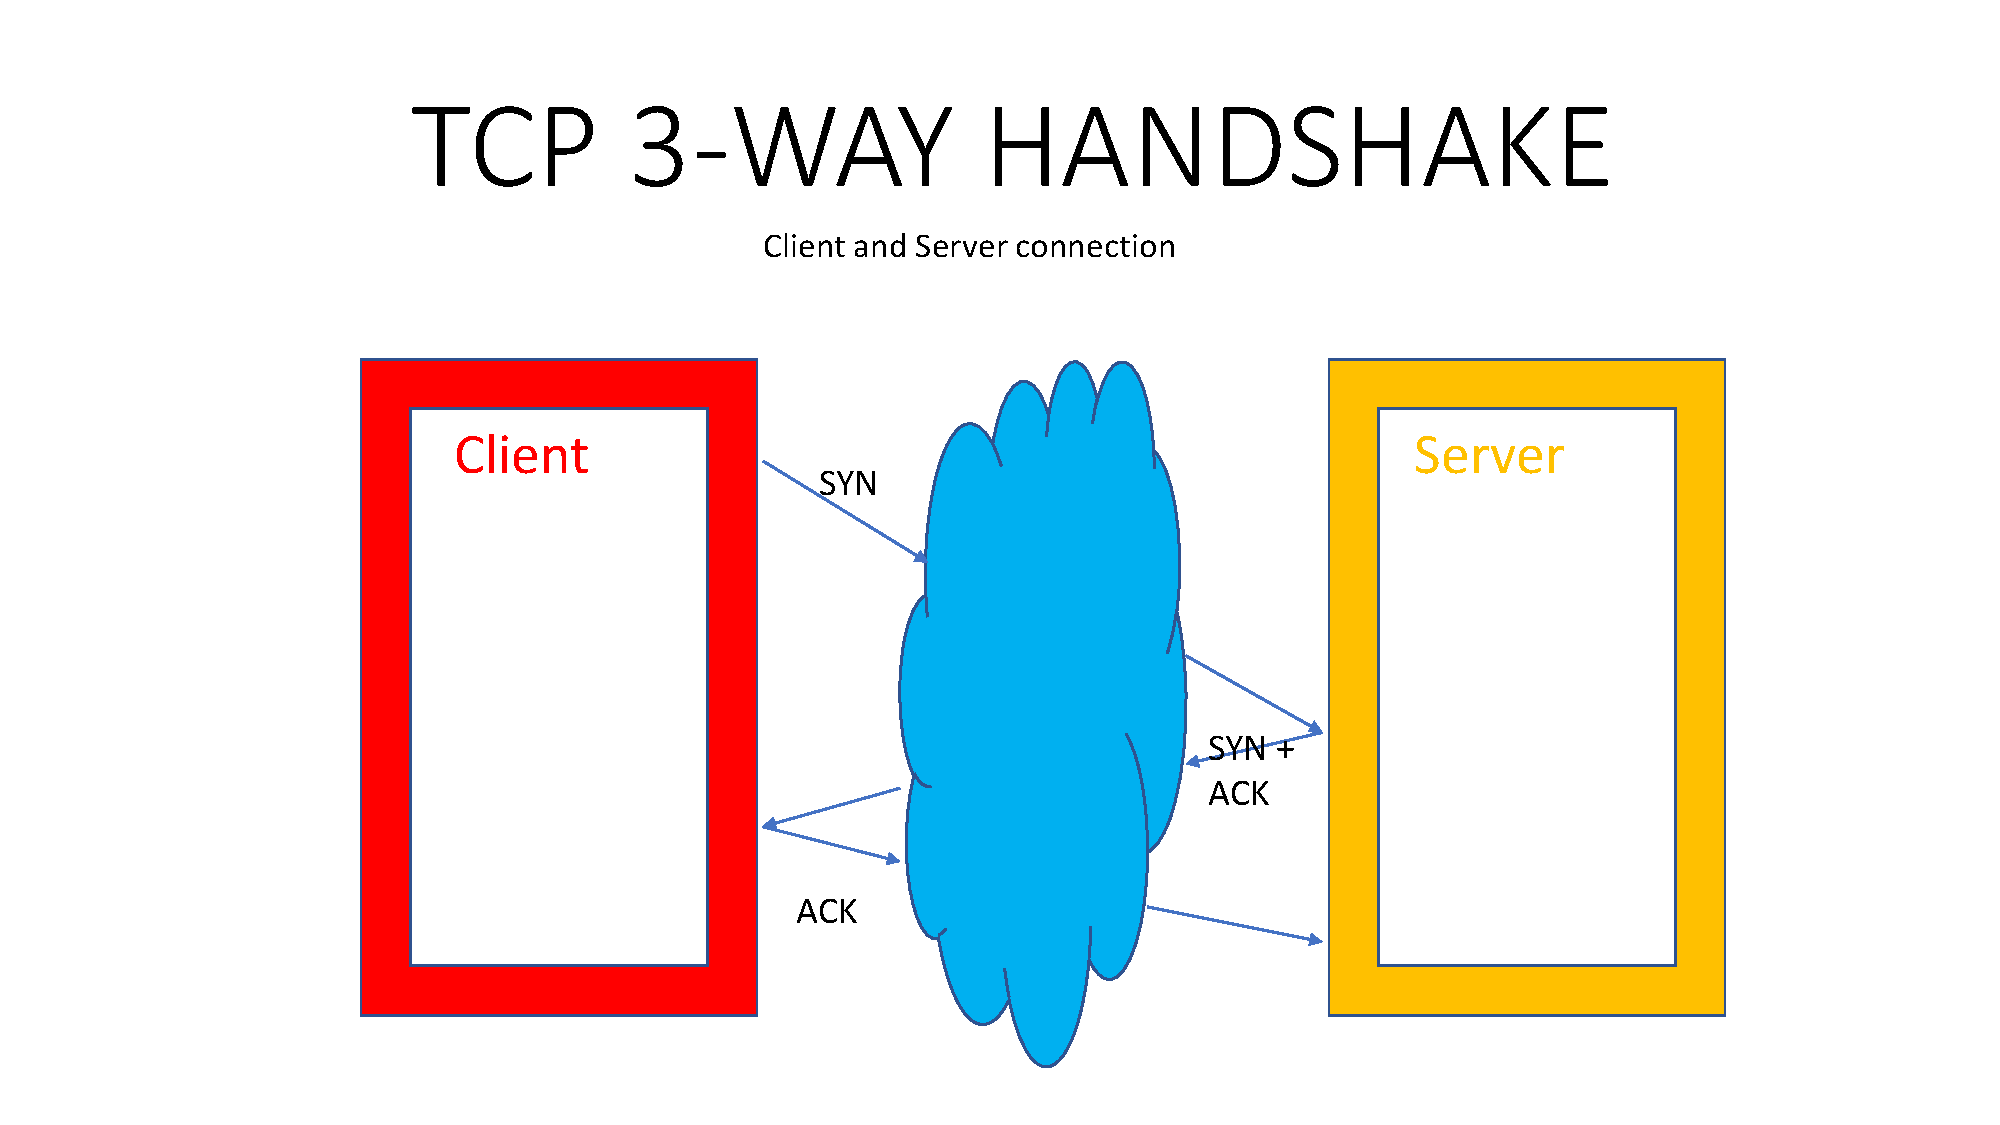
\includegraphics[width=1.0\textwidth]{3way.pdf}
    \caption{TCP three-way handshake. }
    \label{3way}
\end{figure}


\begin{figure}[h]
    \centering
    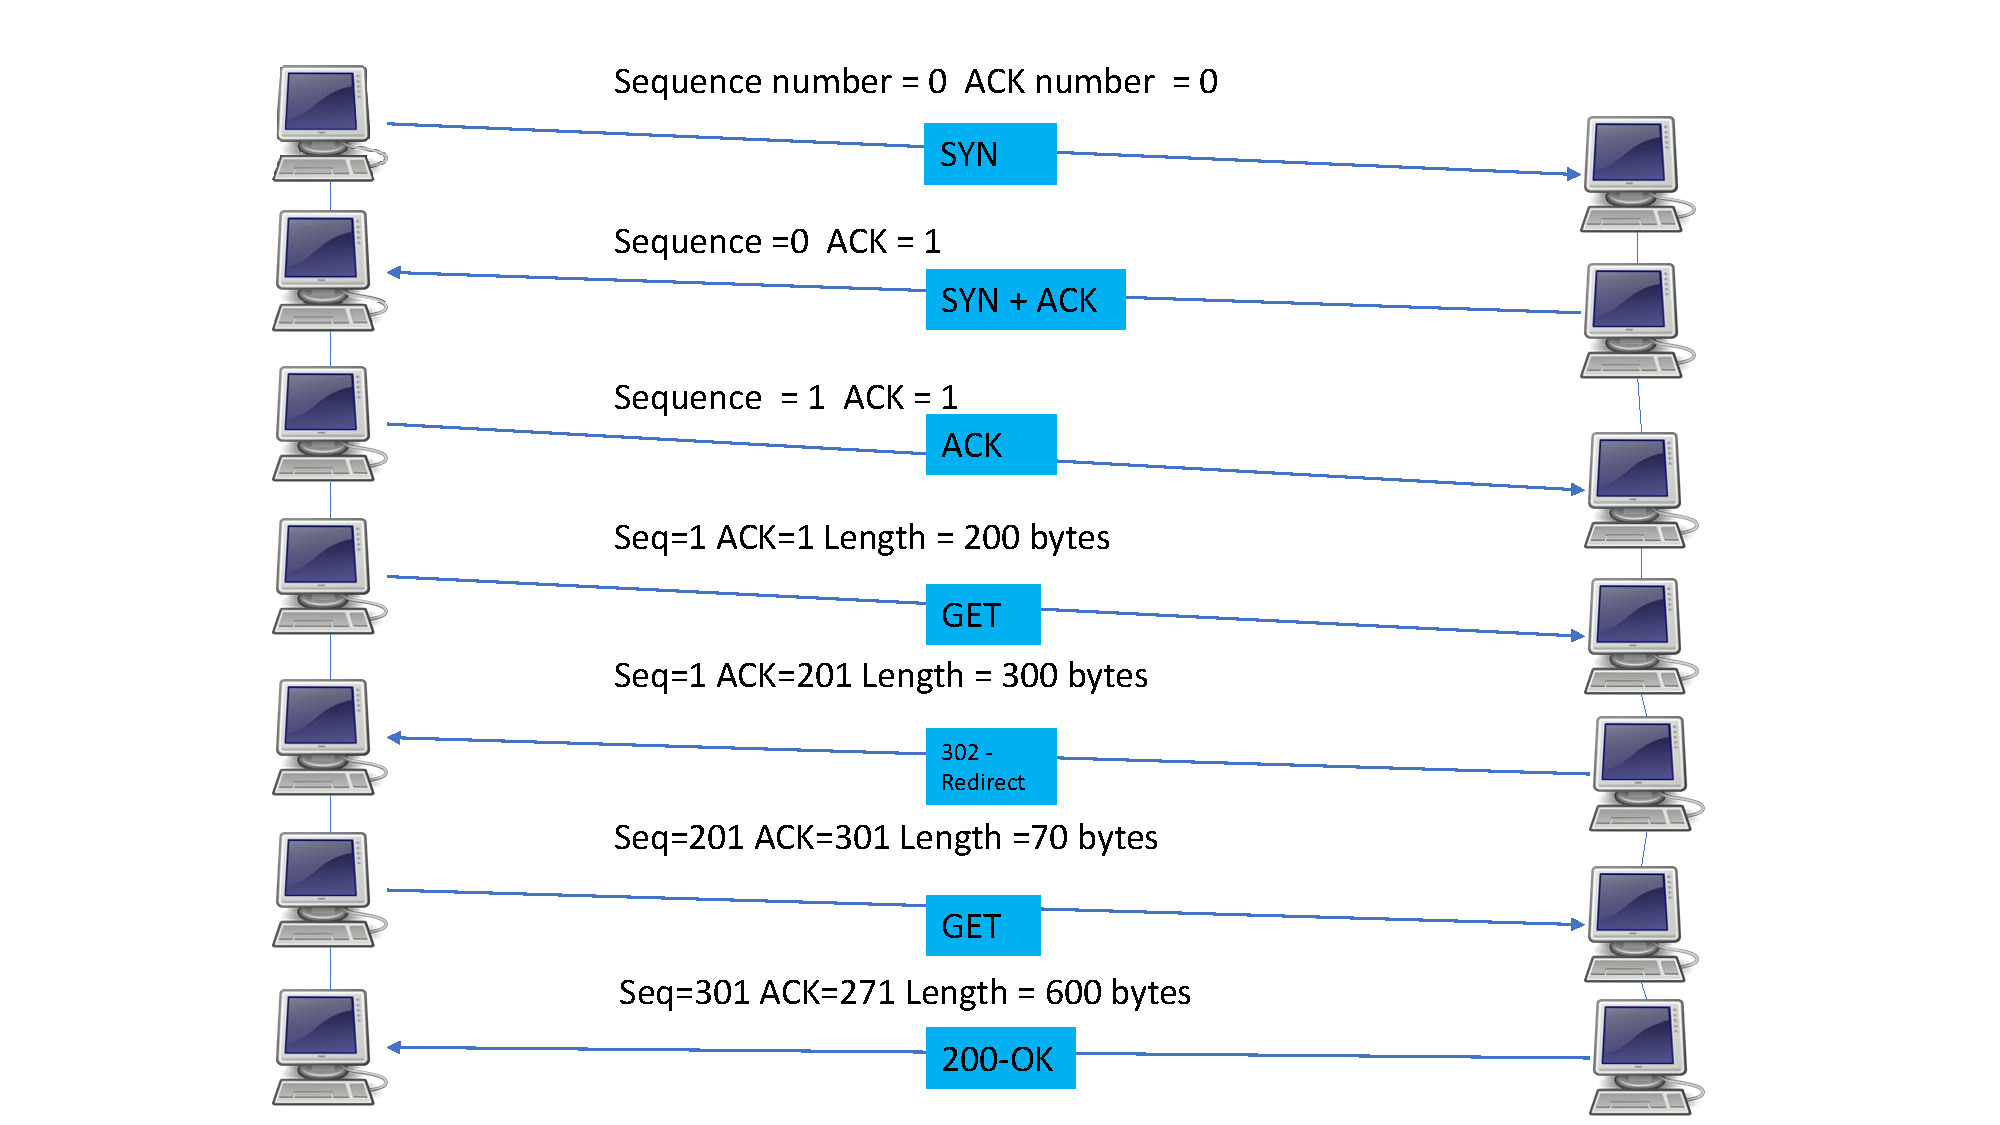
\includegraphics[width=1.1\textwidth]{ACK.pdf}
    \caption{Reliable Data Transport}
    \label{Reliable}
\end{figure}

\section{TCP Traffic Control Methods}\label{TCP Traffic Control}
Now that we have been given a brief overview of TCP and how it works, let us look into the aspect of TCP that relates to the main problem we are examining in this thesis, namely that of latency in narrowband satellite links. 

\subsection{TCP flow control}\label{TCP Flow Control}
TCP Flow control was invented in 1988 by Van Jacobson in response to the Internet's first ever congestion collapse in 1986 on a link from LBL to UC Berkeley ~\cite{19}. This collapse was caused by the sender sending packets to the receiver faster than the receiver can process them which results in the receiver being overwhelmed and collapsing under the weight of transmission ~\cite{19}. \\

Since then, many forms of TCP flow control have been implemented. TCP flow control, in basic terms, is a way for the receiver of data to communicate to the sender and control the amount of data they send so that they do not get overloaded. TCP flow control is now mandatory on all TCP Connections ~\cite{1}. to mitigate these problems. It performs this function via a sliding window mechanism that enables the adjustment of the data rate retransmission dependent on the destinations \emph{receive window}. The target has a certain amount of bytes that it can store in a TCP buffer space. If the amount of data received exceeds the TCP store buffer space, the result is packet loss which is an undesirable outcome ~\cite{1}~\cite{19}.. \\


As the number of bytes in the destination's TCP buffer space accumulate, they will eventually be transferred up for processing to the Application Layer. This clears some of the TCP buffer space for arrival of new packets. TCP Flow control is used to control data flow in the event the receiver is bombarded with data too quickly. Ideally the arrival rate of new packets should match or be slightly less than the rate at which the application layer programs read and clear data from the buffer for processing ~\cite{2}~\cite{19}.\\

The destination host can let the sender know the amount of available buffer space via the form of an advertised window in an ACK back to the sender. The advertised window or receiver window (rwnd) will be read by the sender so that it does not send any data exceeding the advertised amount of bytes in the next exchange. (If the destination host should get wholly overwhelmed, it will advertise a zero byte window, and this will tell the sender to back off completely. The sender will send \emph{keep alive} packets in response to keep the connection open until the receiver recovers and can free up TCP buffer space again) ~\cite{1}~\cite{2}~\cite{19}. \\

It is analogous to filling a bucket with water if it has a hole in it. If water is poured into the bucket too quickly, it will not drain in time and will eventually spill over. If the water flow is at a steady pace that allows it to drain off enough water to not overflow but also not ever be empty, then we have the desired equilibrium we want. We are using the bucket to its maximum capacity and therefore efficiently ~\cite{1}~\cite{2}\cite{19}. \\

Flow control works on the principle that a fast sender should not overwhelm a slow receiver ~\cite{1}~\cite{19}. This principle, however, is a problem that we do not generally encounter with the narrowband satellite link environment in the Pacific. Most of these satellites have bandwidths that preclude a modern day computers TCP/IP stack from being overloaded with incoming data ~\cite{4}~\cite{5}. In the case of high frequency satellites, which are not commonly used across the Pacific, flow control may become useful as the satellites are able to deliver data to earthbound hosts at GB rates ~\cite{5}. \\

TCP flow control is mentioned here, however, as it will be important in future work development for the PEP (See future work section) where modifications to the receiver window can eventually be made by the PEP to adjust for congestion on the network.

\subsection{TCP slow start/ congestion control}
TCP Slow Start is one of the congestion control mechanisms used by TCP, and it is one we will be dealing with mostly in this thesis as it relates directly to the satellite link problem we aim to resolve. Slow start slightly differs from the TCP flow control from the previous section. TCP flow control prevented the sender from overwhelming the receiver via the advertised window informing the sender of the number of bytes remaining in its buffer. \\

As stated in RFC2001 and RFC5681, old TCPs can make a connection between sender and receiver while the sender injects multiple segments into the network as per the advertised window from the receiver (flow control). This flow control mechanism works well when the sender and receiver are on the same LAN or if the data rate flow is almost identical along the path between them. Problems occur, however, when there are routers and slower links between sender and receiver. An intermediary router would then have to queue packets, and the queue itself is then at risk of being overwhelmed under massive traffic flows ~\cite{17}~\cite{18}. So congestion control deals with intermediate routers along the way that could get flooded and not the receiver (as in flow control). The intermediate routers are more likely to suffer congestion first as they typically carry multiple TCP connection flows and handle more traffic than the receiving hosts ~\cite{18}.\\

\subsubsection*{Reason the satellite link environment needs congestion control}
In the narrowband satellite situation, we have this mismatch of these link rates, as mentioned in the RFCs above, between the senders and receivers. The satellite link is a natural long latency bottleneck that will cause a queueing of packets at the input to the satellite, and it is possible for this buffer queue to be overloaded and run out of space. The bottleneck is caused by the satellites limited transmission rate (bits per second) in comparison to the terrestrial transmission rates feeding into it. The transmission rate is determined by the link's available bandwidth divided by the link's capacity ~\cite{4}~\cite{8}. There are several factors contributing to the creation of the satellites natural bottleneck situation:\\

\begin{itemize}
\item Limited availability of spectrum ~\cite{8}.
\item Limited power of the satellite ~\cite{8}.
\item Signal path loss between satellite and ground. Geostationary satellites have a very high orbit. As a result, it is very expensive to launch them that high. Economic restrictions ~\cite{8}.
\item Distance between satellite and ground ~\cite{8}.
\item Need to keep antenna size manageable ~\cite{8}.
\end{itemize}.
\\

\subsubsection*{Slow Start congestion window (cwnd)}
Slow start is a mechanism designed to mitigate the effects of congestion on a network by keeping either side, receiver or sender, from overwhelming the underlying network ~\cite{17}. We have seen the concept of a receiver window in flow control for receiver congestion (rwnd). Slow start congestion control introduces a congestion window for network congestion (cwnd). TCP uses flow control on both windows to regulate their respective traffic flows. See Figure \ref{cwnd}. \\

\begin{itemize}
\item cwnd: congestion window
\item rwnd: receiver window
\end{itemize}.
\\

As stated in the RFC 3135, the congestion window (cwnd) can be thought of as flow control enforced by the sender whereas the advertised window (rwnd) or receive window is flow control applied by the receiver ~\cite{6}. The congestion window (cwnd) is what we deal with in slow start and congestion control. The sender's evaluation of congestion in the network determines the size of the cwnd. The receiver window (rwnd) is determined by the receiver's amount of available buffer space in the TCP flow connection and is what we discussed in the TCP Flow Control section. The cwnd is maintained by the sender and is the number of packets or bytes that the sender is willing to entrust to the channel without having received ACKs for previous segments ~\cite{17}. \\

The slow start algorithm controls the rate of new packets injected by the sender into the network based on the rate of ACKs received back from the destination end. The slow start mechanism works via the implementation of congestion control at the sender. It has two parameters for this purpose, one being the cwnd (congestion window) and the ssthresh (slow start threshold) which is set to typically 10 packets in current versions of Linux ~\cite{17}~\cite{18}. \\

\begin{enumerate}
\item Congestion Window(cwnd; Initial value is 10 packets)
\item Threshhold Value(ssthresh; 65536 bytes but varies in different systems)
\end{enumerate}.
\\

When a connection between two endpoints is established via the three-way handshake, the congestion window(cwnd) is initialised to one segment of size and waits for an ACK (Acknowledgement). Note that an ACK will tell the sender how many bytes the receiver can accommodate via its advertised window and what sequence number of byte it expects next. TCP calculates the round trip time (RTT) for a sent packet A based on the arrival its corresponding ACK. TCP applies this new RTT to transmitted packet B and typically uses double the newly calculated RTT time as a timer for when it expects to receive the corresponding ACK for packet B. If the sender does not receive an ACK for the said packet B in the expected timeframe, or the sender gets a duplicate ACK from a previously sent packet A ( that is indicating it is still awaiting packet B's sequence number next), TCP will assume that packet B has been lost and retransmit it from cache for sender B ~\cite{1}~\cite{2}~\cite{17}. \\

As per the name, TCP starts slowly by sending a small number of segments initially. When it receives the corresponding ACKs back, it grows its congestion window by using the particular algorithm's growth function. Let us assume for this example that our TCP stack uses an exponential growth algorithm. (These growth algorithms differ between TCP types. E.g. TCP Reno, TCP Tahoe, Cubic etc.) ~\cite{14}~\cite{17}.  If TCP receives ACKs for these initially sent segments, it will double its cwnd which doubles the number of transmitted segments. It will repeat this process of exponentially increasing its cwnd and thus doubling segments sent out each time the sender receives the corresponding ACKs back ~\cite{17}.\\

The cwnd will continue to grow until the sender fails to receive an ACK back during the timeout period, which is an indication to the sender that a packet has been lost, possibly due to its cwnd growing too large and causing congestion. This loss tells the sender to cut back on the number of packets it is currently sending. The sender thus initiates exponential backoff and halves the size of its cwnd window. If it fails to receive another packet, it halves the size again and so forth until it has received all its ACKs. During this time it retransmits packets that are lost ~\cite{17}~\cite{18}.
See Fig 2.4.
\\
\begin{figure}[h]
    \centering
    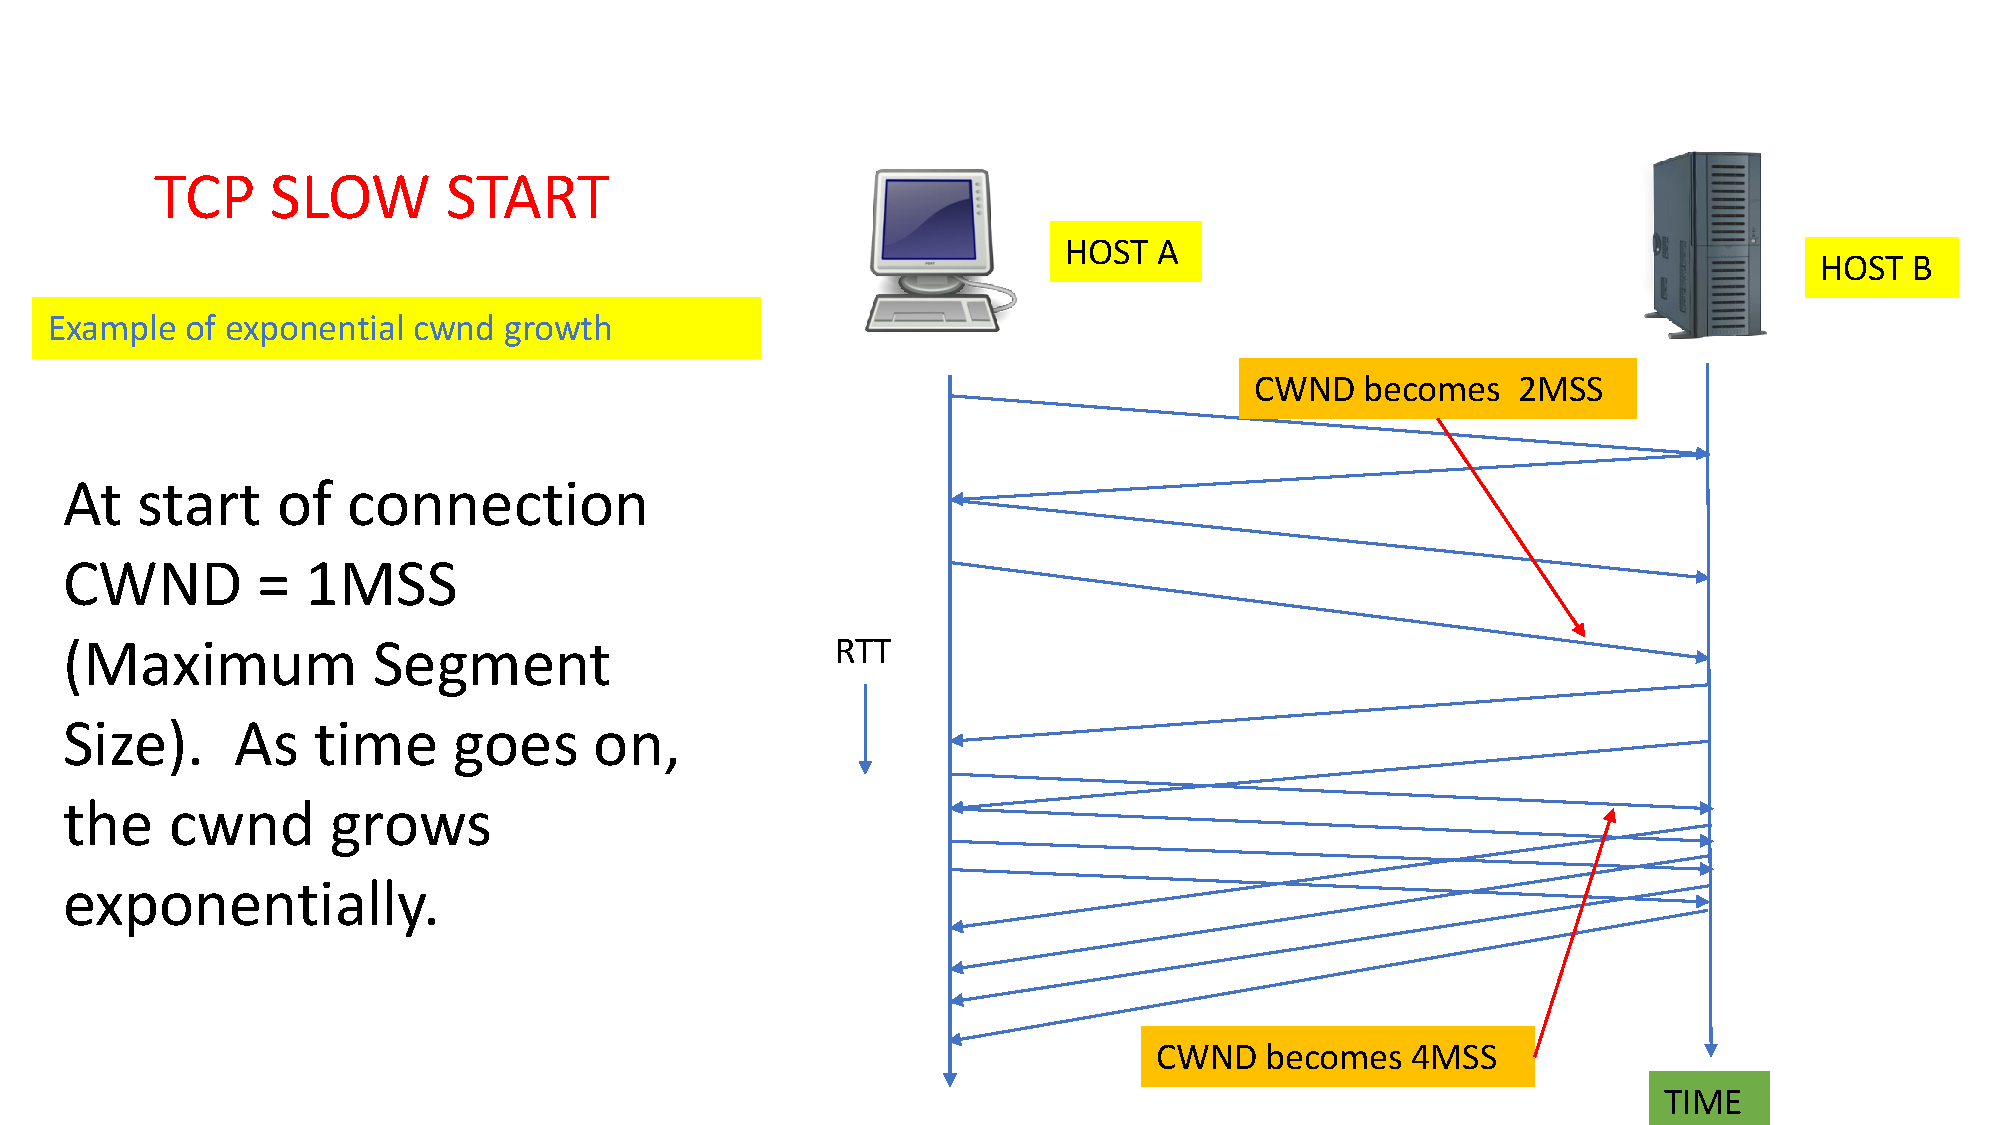
\includegraphics[width=1.0\textwidth]{tcpSlowStart.pdf}
    \caption{Example of exponential tcp slow start}
    \label{cwnd}
\end{figure}.
\\

As seen in Figure 2.5, you can visually see the exponential growth of the cwnd as each ACK comes back and it should increase to the maximum rate (bytes/RTT) allowable by the network as time passes. In a long TCP flow, we have an alternating exchange between exponential growth of cwnd and exponential backoff which should eventually stabilise once the slow start algorithm has settled upon the correct equilibrium for the congestion window. Ideally, this is how the slow start algorithm should work to mitigate against Internet network congestion ~\cite{1}~\cite{17}~\cite{18}, but it does not work so well with satellite link environments ~\cite{14}. In fact, slow start actually compounds the problem of high latency propagation delay with narrowband satellite links because it slows down the growth of the congestion window ~\cite{13}~\cite{14}. \\

\subsection{Slow Start in a satellite link environment}
Slow start becomes an issue in satellite links due to latency caused by the distance the packets must travel as outlined earlier in Section 1.1 "Problem and Motivation" and the bottleneck nature of the satellite link ~\cite{13}. The resultant "queue oscillation" as explained in more detail earlier, is caused by the combination of \emph{slow start}, the latency and the bottleneck network links ~\cite{4}~\cite{5}. \\

In a satellite link environment, the problems we have with slow start are the following; \\

\begin{enumerate}
\item The inherent latency in the link causes ACKs to arrive back to the sender much later (typically 500ms RTT in Pacific Islands). This means that even if there is no congestion on the link, slow starts cwnd in this environment grows more slowly than a typical terrestrial based TCP cwnd. The first time our senders in Pacific region, for example, can grow their cwnd is after 500ms or slightly longer depending on how far the host is from the satellite link ~\cite{4}~\cite{8}. \\
\item As the congestion window has been increased, ACKs may be returning even while the queue is overflowing because these are ACKs pertaining to packets that got through the satellite link before the queue flooded. The sender receives the ACKs believing its cwnd is too small and so TCP increases the cwnd sending more packets to an already overflowing queue. The latency in the link means that the sender will not learn about the overflowing queue for another 500ms, or longer depending on the TCP variants tolerance to lost packets. During this time, the sender will drop a large percentage of sent packets ~\cite{4}~\cite{8}.\\
\item For these lost packets, the sender will get ACK timeouts which will trigger exponential backoff. The sheer volume of packets lost due to the late discovery of the queue overflow will result in a radical decrease in sender output. Every lost ACK results in a halving of the congestion window so the sender output volume decreases rapidly until almost nothing is being outputted ~\cite{4}~\cite{8}.\\
\item  In the satellite environment, there is synchronisation between TCP senders that does not exist in the terrestrial TCP landscape.In a normal earthbound router, there are TCP flows with a mix of latencies traversing across it with different hosts receiving their ACKs at different times. Hosts in a normal network would not all ramp up their output( via slow start) or  back off at the same time. Hosts connected in a satellite link, however, all back off and ramp up simultaneously as they all receive the same outdated idea of what is happening at the satellite input queue ~\cite{4}~\cite{8}.\\
\end{enumerate}

These factors compound and perpetuate the extreme "queue oscillation" problem mentioned earlier in section 1.1. The pattern of perpetual oscillation and sawtooth patterns in network transmissions is generally of an acceptable level ~\cite{5}. In a normal terrestrial network, we have relatively low latency so the sender can get information back on dropped packets/congestion sooner and can, therefore, readjust their cwnd very quickly to suit the network conditions ~\cite{1}.\\

TCP in a typical environment can also increase the cwnd much faster as they receive the ACKs quickly due to low latency. The regular queue oscillation would occur almost entirely within its queue buffer. An overflowing and an empty buffers would be very shortlived, and filling of the buffer would be relatively slow, so packet loss is minimal ~\cite{1}~\cite{2}. If we were to print out the oscillation sawtooth pattern for a host in a standard network on an A4 sheet of paper, we would see a patterned sawtooth picture with several teeth per second running across the page. The peaks would represent the slow start cwnd ramping up very quickly, and the valleys represent the back off which also happens quickly ~\cite{1}~\cite{2}. \\

However, in narrowband satellite link transmissions, we are concerned with the extreme depth of the sawtooth pattern because the excessive burst packet losses can cause extreme backoff from all connected hosts at the same time resulting in severe link underutilisation ~\cite{4}~\cite{5}. The hosts then all ramp up again at the same time, growing their cwnd simultaneously.The satellite line queues fill quickly due to the combined influx of packets from all connected hosts ramping up simultaneously, thus repeating the cycle. If we were to print out the oscillation sawtooth pattern for a host in a satellite network across the same A4 paper, we would see a sawtooth pattern comprised of maybe one or two teeth per second with extremely high peaks representing a slow climb to grow its cwnd to a maximum. We would also see equally low valleys representing the rapid descent from exponential back off. This extreme queue oscillation and the subsequent inefficient usage of the link is a common problem with narrowband satellite links and is the main problem that this thesis aims to resolve ~\cite{4}~\cite{5}~\cite{8}.\\

So in summary, we have a bottleneck narrowband satellite link that is continuously facing two issues. Firstly, packets are continually being queued at the sender end due to the bottleneck nature of the link. The satellite link's latency means that ACKs get back too late to the sender. This lateness can cause problems 1 and 2 listed above whereby excessive sender backoff starves the the satellite uplink queue as all the senders stop emitting packets altogether for a period of time. This is an inefficient use of the link, and it is caused directly by the slow start backoff algorithm ~\cite{5}~\cite{15}. \\

Secondly, we have the issue of the cwnd window of all the senders ramping up in unison as they receive a multitude of ACKs that had been expected but assumed dropped and been retransmitted. The connected hosts all begin growing their cwnd at the same time which fills the bottleneck link queues up quickly and subsequently leads to the continual cycle of ramp up/ramp down again. The resultant extreme queue activity results in extremely small congestion windows for large flows. Once again, the propagation latency, caused by the vast distances that had the sender sending too much for too long, now conversely has it emitting too little for too long ~\cite{5}~\cite{15}~\cite{16}. \\

Generally, satellite TCP connections are known to be susceptible to network congestion and so this has become the subject of much research and experimentation over the years ~\cite{14}~\cite{16}. The universal consensus in the scientific community is that TCP satellite link environments are somewhat problematic and many different solutions have been created to mitigate these problems ~\cite{14}~\cite{16}. This thesis will concentrate on the development of a non-connection breaking PEP platform which will attempt to mitigate these problems.\\

\subsubsection*{The effects of TCP long flows and short flows in satellite link environments}
There are scenarios where the satellite link is underutilized even in the absence of excessive queue oscillation. TCP short flows are defined as flows that last less than one RTT. A 1Kb flow from a webserver where the connection is alive for the period of an HTML webpage transfer is a good example of such a flow ~\cite{5}~\cite{20}. These short flows do not allow TCP congestion control mechanisms such as \emph{slow start} the chance to grow its congestion window whereas long TCP flows last several RTT's last long enough to provide feedback to the TCP congestion mechanisms ~\cite{5}~\cite{20}. It is possible to have a scenario where these a massive surge of these short flows fill the queues and cause packets loss for long TCP flows on the link which causes excessive backoff to the point where they no longer send any data while only the short flows manage to get through ~\cite{5}~\cite{20}. This is a somewhat rare case, however, which our thesis will therefore not address.


\subsection{Pacific Islands Internet speeds}

Most of the Pacific island region used to rely on a single satellite each for all its islands Internet connectivity but some islands have recently gone through some upgrades with a few of the islands using undersea cables for its Internet (Samoa, Tonga, Fiji, parts of French Polynesia etc.) ~\cite{3}. However, there remain many islands that still rely on satellites for Internet, and they suffer from much lower performance as a result. Technological advances in Internet technology that affect social media, hospitals, business, banking  and just about every other facet of modern life requires the corresponding Internet performance to fully maximise the benefits. This provides a strong motivation to improve Internet access in the Pacific Islands that cannot afford undersea cables and this thesis looks at ways of doing this at minimal costs ~\cite{3}~\cite{4}.

\todo{(Placeholder- reminder to self- find some data-graphs etc. showing recorded speeds of internet in islands to put here)-expand on this part later)}

\subsection{Other concepts used in this thesis}\index{Related topics}
This thesis will only give a brief overview of the C programming basics and TCP as we will focus on the proposed PEP and its functionality. Readers unfamiliar with the topics below may wish to refer to a good C programming book or the respective literature cited in this thesis for a more in-depth treatment.

\begin{itemize}
    \item C Programming
        \begin{itemize}
            \item pointers in C 
            \item structs in C 
            \item socket programming in C
            \item raw socket programming in C
        \end{itemize}
    \item satellite speeds in the Pacific Islands
        \begin{itemize}
            \item history of Pacific island Internet Infrastructure
            \item latency in satellite links
            \item current Internet performance in the Pacific region
        \end{itemize}
    \item TCP
        \begin{itemize}
            \item History of Internet Protocols/TCP
            \item TCP Congestion Control/Flow Control
            \item TCP Reno/ Cubic/ Vegas-TCP Hybla etc
            \item TCP clients and servers
            \item OSI layers
        \end{itemize}
   \item PEPs
         \begin{itemize}
            \item PEP Databases online- RFC 3135, 3155
            \item TCPep
            \item PEPsal
        \end{itemize}
\end{itemize}


% chapter 3: Network Measurement
%----------------------------------------------------------------------------------------
%	CHAPTER 3
%----------------------------------------------------------------------------------------

\chapter{LITERATURE REVIEW}

This section looks at the relevant related work that has been employed previously to resolve satellite Internet delays and takes a look at three past implementations of PEPs. Section 3.1 gives a brief overview of performance enhancing proxies. Section 3.2 provides a brief recap of the satellite links issues and Section 3.2.1 delves into the research conducted to try to resolve these issues with a focus on PEPs. Section 3.3 and its various subsections detail the PEP categorisations. Section 3.4 compares and contrasts three past PEPs with each other and the PEP in this thesis. Section 3.4.1, 3.4.2 and 3.4.3 examine PEPsal, TCPep and FastSAT respectively.

\begin{figure}[h!]
    \centering
    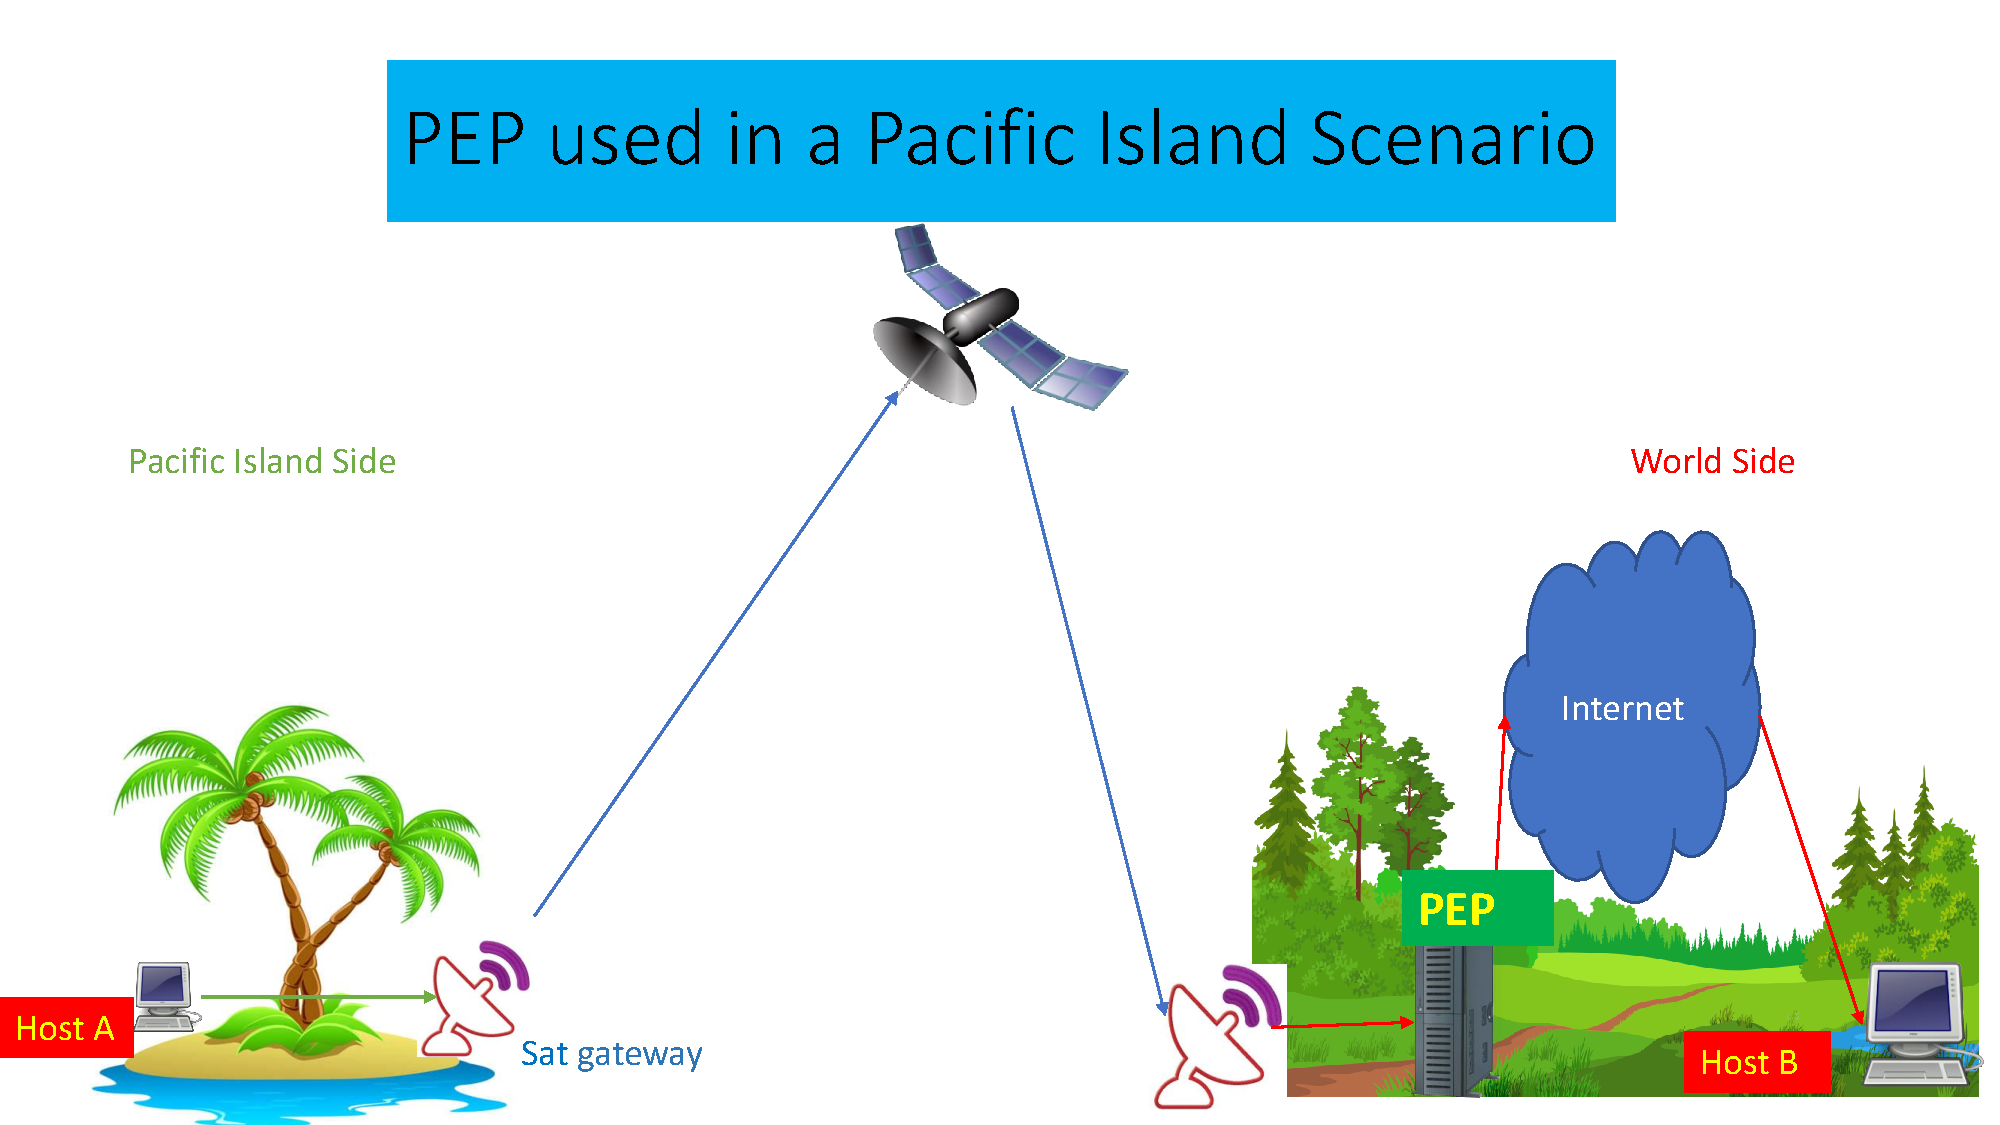
\includegraphics[width=0.95\textwidth]{PEP.pdf}
    \caption{Single PEP on the Island network}
    \label{IslandPEP}
\end{figure}.

\section{Performance Enhancing Proxy}\label{Proxy}
Performance Enhancing Proxies (PEPs) are a technology utilised to prevent the degradation of TCP performance over links with long latencies, such as in the case of TCP over bottleneck satellite links in the Pacific islands ~\cite{6}. (Commercial PEPs are proprietary, so they do not advertise their methods for achieving this). In simple terms, a Performance Enhancing Proxy (PEP) sits between two hosts that are communicating. More precisely, the PEP sits between one host and the degraded link connecting it to the other host ~\cite{6}. In our case, the narrowband bottleneck satellite link is the degraded link connecting our hosts. The PEP is used to effectively give the illusion of shortening the latency between the two hosts and thus mitigating the problems associated with connection latency over a narrowband satellite link. The PEP does this, in most cases, by breaking the connection between the hosts while establishing its own connection with the hosts ~\cite{14}. This type of PEP is called a \emph{connection breaking PEP} and is the most widely and commonly used PEP ~\cite{6}~\cite{14}. Figure \ref{IslandPEP} and \ref{DistributedPEP} give us a visualisation of where the PEP sits in the infrastructure.

\begin{figure}[h!]
    \centering
    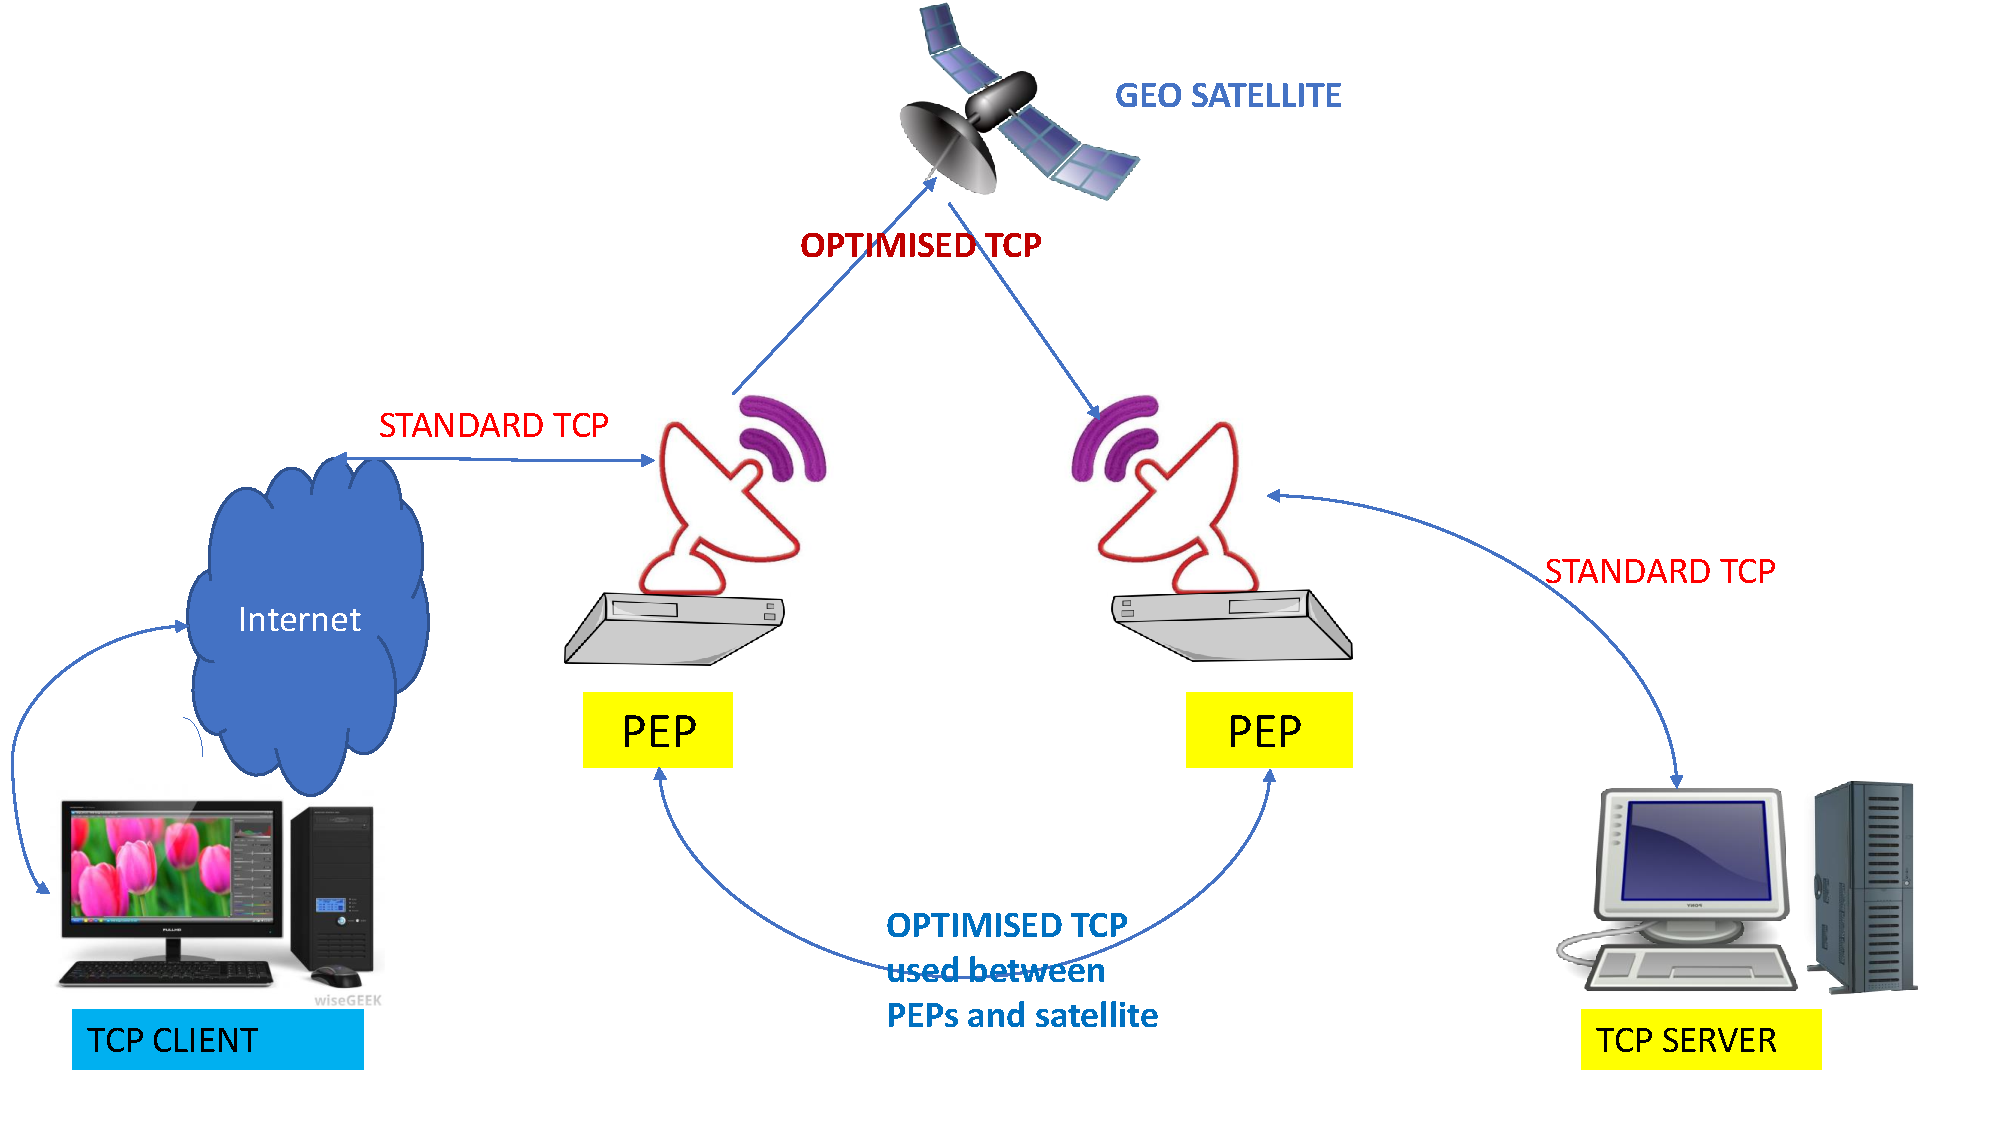
\includegraphics[width=0.9\textwidth]{DistPEPs.pdf}
    \caption{PEP 2nd Diagram}
    \label{DistributedPEP}
\end{figure}

Figure \ref{IslandPEP} shows the PEP sitting between the router of one host endpoint and the satellite link and the other endpoints router and its satellite link. This singular PEP is set up on the world facing side of the satellite link. This is how the PEP in this thesis will be implemented.  \\

Figure \ref{DistributedPEP} shows us a typical visualisation of the TCP client/TCP server connection between client and server. We see satellite connections between client and server is broken up by PEPs in between client and server on both sides of the satellite link. The picture represents the typical set up of a commercial PEP which uses its own proprietary algorithms to optimise the satellite connections ~\cite{6}~\cite{14}. The example here is a TCP client and a ship. Our thesis will focus on the benefits of using the PEP in the Pacific Island environment, but the research is also beneficial for planes and ship satellite communications. \\

\section{History of Satellite Link Issues And Proposed Solutions Including PEPs}\label{History}
Satellite link issues with regards to Internet connectivity, has been fraught with a long history of challenges. The primary culprit behind these challenges is the link latency caused by the long propagation channel between satellites and their terrestrial counterparts in the communication chain. Thus far, this thesis has already detailed the various historical issues/challenges with satellite links. This section will look at the history of proposed solutions resulting from research into these challenges, including PEP variations (Later in this chapter, we will look specifically at past PEP implementations, both open source and commercial). \\

Before we discuss the negatives of satellite links, we should first look at its positives. Satellites can cover extensive geographical areas and can thus provide Internet broadband connectivity to remote areas such as the Pacific Island nations ~\cite{15}. These islands are very difficult to reach via terrestrial infrastructures, with Samoa and Tonga being some of the few islands able to get access to fast broadband connectivity via expensive undersea cables. Most Pacific islands cannot afford this and thus satellite Internet connectivity is the only option at the moment ~\cite{3}~\cite{4}. \\

So while satellites connection are advantageous in some respects, they also have had a long history of challenges in the form of "high delay-bandwidth product, low signal-to-noise ratio, long feedback loop, transmission error, variable Round Trip Time (RTT), and intermittent connectivity" ~\cite{15} which all contribute to extreme queue oscillation. These issues certainly have an adverse effect on the satellite networks quality in terms of Internet connectivity (IP Protocol) ~\cite{15}. \\

Given the length of time satellite latency and the resultant queue oscillation, has been a known problem (over 30 years), one may wonder why there is no clear-cut resolution given over the many years of research. With advancements in technology, it would seem like a solution for our Pacific Island problem would have been found by now ~\cite{21}. \\

The answer has more to do with the socio-economic status of the Pacific Island region in comparison with the rest of the Internet connected world and the general history of satellite Internet. Satellite connections in the 1980s and 90s, or Internet connectivity in general, were not as prevalent in the Pacific as they are now which meant less traffic on the link. Furthermore, Internet data rates, in general, were much slower in the past, not only for the Pacific but most terrestrial network connection. Dial-up speeds were the norm on land in so so the reduced traffic combined with slower rate Internet would have meant we had much less of a bottleneck in the satellite link s of the day to perhaps prompt a need for an urgent fix ~\cite{21}. Even today, in Rarotonga, we only witness queue oscillation when there are over 2000 parallel inbound TCP flows ~\cite{4}. \\

As the Internet became more of a commodity worldwide by the late 1990's, many more millions of users connected to the Internet, so more investment was made into building satellites capable of meeting this demand. The satellites were built with capacities to be able to deal with the size of the terrestrial networks connecting to them and thus effectively removing or significantly reducing any bottleneck effect and eliminating most, if not all, the adverse effects of satellite link latency ~\cite{21}.\\

This leads us back to the present day and the issue of socio-economic status in the Pacific Islands. The number of Internet users on the islands has grown considerably since the 1980s and 90s meaning that they can now generate a significant amount of Internet traffic (parallel TCP sessions) over the link ~\cite{21}. However, unlike their western counterparts such as New Zealand for instance, many of these Pacific Island nations cannot afford the satellite capacity it takes to eliminate a bottleneck link. Hence the need to find a cheap alternative to mitigate the problem for them ~\cite{3}~\cite{4}. 

\subsection{Historical solutions for satellite link issues}

Researchers have proposed many solutions over the years to mitigate the challenges posed by satellite link connections for the Internet ~\cite{7}~\cite{9}. The body of work brought about in trying to resolve these challenges is vast and complex. Instead of trying to summarise the entirety of this enormous body of work in detail, which would consume the remaining space of this thesis, this section will provide surface detail of the type of solutions presented accompanied by references to allow a more comprehensive investigation by the reader if so desired. \\

A recap and summary of the two main problems with satellite links as per the previous chapter:\\

\begin{itemize}

\item Random lossy links unrelated to congestion happen too often to be ignored. Their frequent occurrence and impact on network performance must be taken into account. Error rates have been reported to be as high as 1 in 10-5 which is comparatively much higher than terrestrial routes ~\cite{22}~\cite{25}. TCP regards all losses as due to congestion which triggers the backoff algorithm.

\item The RTT is increased by the large propagation latency to a number that is significantly large enough to cause problems in the network as previously discussed (GEO RTT is typically at 500 ms or slightly above). Excessive queue oscillation and subsequent major packet loss and link underutilisation results from the sender not being able to gauge the state of the link as quickly as it does on terrestrial links ~\cite{7}~\cite{9}.\\

\end{itemize}

Recall that these two factors combine to cause significant problems for the transport layer TCP reliability ~\cite{7}~\cite{9}. TCP \emph{slow start/congestion avoidance} mechanism is severely disrupted resulting in inefficient behaviour typified by unnecessary retransmissions and false timeouts ~\cite{8}~\cite{15}. 

Several research avenues have been explored to solve the abovementioned problem and can be categorised as either improvement to TCP involving only the end hosts ~\cite{10}~\cite{26} or TCP enhancements via the use of PEPs ~\cite{6}~\cite{14}. \\

An option that has been explored is to make TCP more intelligent so that it can distinguish between losses caused by congestion and losses resulting from random datagram errors ~\cite{23}. NASA provided funding for experiments of this nature where \emph{explicit error notification} can be used for satellite links. This would help reduce the backoff algorithm from being triggered prematurely and allow faster opening of the cwnd ~\cite{13}~\cite{23}. So far, results from these studies have not been released publicly or commercially as far as this author is aware. \\

Another TCP extension/improvement was aimed at improving retransmission times but more importantly, enabling TCP to have a better assessment of the available path bandwidth after a period of successive losses via selective acknowledgements (SACKs) ~\cite{24}. Though not explicitly developed for satellite networks, the retransmission efficiency it offers can at least help alleviate one aspect of the satellite link problem.\\

The use of the forward error correction properties of a network code was recently proposed as a solution to the satellite link problem and tested specifically for the Pacific Island region ~\cite{4}~\cite{5}. The network coding was shown to improve TCP performance over a satellite link by hiding packet losses between two TCP hosts on opposite sides of the link ~\cite{4}~\cite{5}.\\

From the TCP improvements proposed via the use of PEPs ~\cite{6}~\cite{14}, the connection breaking/TCP splitting PEPs have been touted as the most effective option by some researchers ~\cite{14}, but they also have their problems. In breaking the fundamental end to end semantics of TCP, they can cause many adverse side effects ~\cite{6}. The TCP PEPs can also be categorised as either integrated or distributed, open source or commercial. This section will only discuss these categorisations briefly, but they will be covered in more depth in Section 3.3 \emph{Pep Catergorisations}.\\

An integrated PEP sits on only one side of the satellite link which is the side representing the last hop for Internet access. These PEPs use TCP or an optimised version of TCP over the satellite leg of their link path and usually require no software or hardware modification to the receiver end ~\cite{6}~\cite{14}. A distributed PEP sits on both sides of the sat link and can, therefore, use a custom transport protocol other than TCP across the satellite link itself. Most commercial PEPs use or permit a distributed architecture ~\cite{6}~\cite{14}. \\

The PEP in this thesis will be open source and using an integrated architecture with TCP for testing and experimentation (although it can also be modified to be used in a distributed architecture too) but will be non-connection breaking. For this reason, this thesis will not be focused on TCP splitting options ~\cite{14}~\cite{27}~\cite{28}. This research will also not focus on commercial implementations of PEPs ~\cite{29} as the source code is proprietary and will also disregard open source distributed PEPs, that use their own specialised transport protocols such as SCPS ~\cite{11}. \\

The PEP in this thesis also uses TCP whereas a past PEP implementation called PEPsal, for instance, uses an enhanced form of TCP called TCP Hybla which has been optimised for better performance to suit satellite links ~\cite{14}. This thesis will only focus on the performance of the PEP itself using standard TCP variants. This PEP is also tested and run on Linux, similarly to PEPsal, PEP solutions not available for Linux will not be considered here. ~\cite{30}~\cite{31}~\cite{32}. \\

The open source non-connection breaking PEP in this thesis is the first of its kind implemented in Linux as far as this author is aware. The next section (3.3) will explain the prior mentioned PEP categorisations in more detail. Then the following section will compare and contrast previously implemented PEPs, such as the previously mentioned PEPsal, with our non-connection breaking PEP. \\

\section{PEP Categorisations}
As part of the literature review on PEPs, it is important to know the PEP categorisations currently in existence. This knowledge helps the reader understand how my PEP is categorised and also how it differs from other PEPs. Generally, the use of PEPs is not recommended unless in an environment where there are no other viable options to improve link performance ~\cite{6}. The consensus is that the fundamental end to end principle of the Internet should always be adhered to where possible and most PEPs break end to end connectivity ~\cite{6}. As mentioned in the introduction, the PEP in our thesis partially addresses this issue as it is an experimental non-connection breaking PEP. Therefore our first categorisation will be for connection breaking PEPs as this has high importance to this thesis. 

\subsection{Connection breaking PEP}
A connection breaking PEP is also referred to as a \emph{TCP splitting PEP} in many manuals. As described in RFC3515, a split connection TCP implementation mimics the endpoint or target host/server of the connection/packet in both directions, thus literally splitting the connection in half (TCP splitting). In an integrated TCP splitting PEP "the PEP... terminates the connection from one end system and originates a separate connection to the other end system" ~\cite{6}. The PEP is managing two separate connections simultaneously so that the endpoints operate as if they are communicating directly with each other. \\

Simply put, the communicating hosts believe there is no middleman. (see Transparency Type below). For example, the intercepting PEP receives a data packet and sends acknowledgements back to the sender to say it has received the packet. The PEP also suppresses the real ACKs coming back from the receiver of sent packets on either side of the split connection. The PEP then forwards the payload data from the packet to the intended target and vice versa ~\cite{6}~\cite{14}. It is essential to keep in mind the connection-breaking concept as the novelty of the PEP in our thesis is the fact it is a non-connection breaking PEP. It is also the first open source non-connection breaking PEP. In Section 4.3.1 "Non-Connection Breaking PEP", this thesis will provide more detail on the reasons for having this as our novelty. These details include the problems inherent in breaking the Internet's fundamental rule of end to end connectivity and the methods utilised by our PEP to partially mitigate these issues. \\

\subsection{PEP distribution type}
There are two types of PEP distribution types:\\
\begin{itemize}
\item Integrated 
\item Distributed\\
\end{itemize}
An Integrated PEP is a single PEP component that connects between a host and the degraded link. The PEP is one node in the connection between the TCP hosts and the degraded link between them. The performance of the link is enhanced at that singular point where the PEP sits. The advantage of having an integrated PEP is that it is a single box and it is neither hardware, software or operating system specific. It is also inexpensive to run and easily maintained or upgraded because it is merely some code sitting on a computer that interacts with the switches/routers ~\cite{6}~\cite{14}. The disadvantage for integrated PEPs is that they only allow standard or advanced TCP protocols on the satellite which means they would have to exclude all proprietary solutions. Even the use of advanced TCP protocols (TCP Hybla etc.) designed for improved performance on a satellite link is somewhat limited as the receiving hosts have to be compatible with this enhanced TCP variant to reap the benefits. Figure \ref{IslandPEP} is an example of an integrated PEP architecture.\\

Distributed PEPs sit on both sides of the problematic link and even on the satellite itself. You could also have a chain of several PEPs along the communication link. This setup is typical with commercial PEPs who use their own proprietary protocols and algorithms, sometimes instead of TCP, to communicate between their proxies. As stated in the PEPsal article, by surrounding and "isolating the satellite link between two PEP agents...it is possible to adopt a proper transport protocol on the satellite link, such as SCPS" ~\cite{14}. SCPS stands for \emph{Space Communications Protocol Specifications}, a non-TCP protocol designed specifically for satellite link traversal ~\cite{11}. Similar proprietary protocols can be applied to this distribution architecture. Figure \ref{DistributedPEP} is an example of a distributed PEP architecture.\\

The PEP in this thesis can be operated both as an integrated type and a distributed type of PEP. 
 
\subsection{PEP layering type}
There are two types here: \\
\begin{itemize}
\item Transport Layer PEPs
\item Application Layer PEPs\\
\end{itemize}

According to RFC 3135 "transport layer PEPs operate at the transport level...they do not modify the application protocol(e.g. HTTP) in any way, but let the application protocol operate end-to-end.  Most transport layer PEP implementations interact with TCP" ~\cite{6}. This is what is known as a TCP PEP and interacts with the TCP Protocol. In environments where we have bursty traffic or prolonged bandwidth delay (as in the case with satellite links) this type of proxy modifies/alters/enhances the TCP behaviour. It can increase ACK spacing to counter bursty traffic that leads to inefficient use of the bandwidth. Alternatively, it can generate local ACK responses to improve the throughput of the link (See previous "Connection Breaking PEP" section for more detail).\\

Application Layer PEPs operate at the application layer (above the transport layer). These types of PEPs are widely used today like Microsoft Proxy Server; the Web Proxy Service is an application layer proxy for the Hypertext Transfer Protocol (HTTP), relay Mail Transfer Agents (MTA) and cache proxies that are used to optimise performance and service availability ~\cite{6}. Application Layer PEPs will not be helpful for dealing with the narrowband satellite link problem in our thesis as it has no bearing on the satellite link issues. PEPsal and TCPep are also \emph{transport layer PEPs}. This thesis will focus only on Transport Layer PEPS.

\subsection{PEP symmetry type}
As defined in RFC3135, a PEPs symmetry type can be either:

\begin{itemize}
\item Symmetric
\item Asymmetric
\end{itemize}

Symmetric PEPs treat both sides of the connection exactly the same, so that the PEPs optimisation is propagated in both directions. Assymetric PEPs treat both sides of the connection differently so that only one link direction performance may be optimised ~\cite{6}. As in the case of the PEP in this thesis, for example, which takes into account one of its sides is facing the satellite link and the other side is facing the island side ~\cite{4}~\cite{5}.  The island senders are on the same side of the satellite connection as the PEP (usually the world side in satellite connections to small islands, ships etc. because this is where most of the data volume comes from) which ensures the quickest ACK returns for the sender's data packets ~\cite{4}. Thus our PEP is assymetric as the link optimisation occurs in the direction facing the island side. See Figure \ref{IslandPEP}.  \\

\subsection{PEP transparency type}
Transparency here is defined as whether the end systems, endpoints, applications or users are aware of the PEP or does the PEP operate entirely transparently/invisible to them. If a PEP requires modifications to be made to any of the end systems, endpoints or applications, then it is considered non-transparent ~\cite{6}. The PEP in our thesis is transparent.

RFC3515 categorises the degree of transparency a PEP can have:\\
\begin{itemize}
\item transparency with respect to the end systems (network-layer transparent PEP) ~\cite{6}.
\item transparency with respect to the transport endpoints (transport-layer transparent PEP) ~\cite{6}.
\item transparency with respect to the applications (application-layer transparent PEP) ~\cite{6}.
\item transparency with respect to the users ~\cite{6}.\\
\end{itemize}

        
\section{Past Implementations Of PEPs}

In this thesis, we show our version of a PEP that uses a non-connection breaking PEP to mitigate the problems with satellite link latency. Before we do this, however, this section examines other PEPs that have been developed and implemented in the past and then finally shows how our version differs.\\
 
List of PEPs considered in this section:
 \begin{itemize}
 \item PEPsal
 \item TCPep
 \item Commercial PEPs
 \end{itemize}
There are many more, but we will restrict ourselves here to the treatment of the two open source PEPS above and a general overview of commercial PEPs which often do not have much detail available for the public. The reader may want to refer to section 2.2.5 "Other Concepts Used In This Thesis" for further information on this topic.

\subsection{PEPsal}
PEPsal was initially developed as part of a research project for experimentation in a university but has since been successfully adopted by a US satellite provider used by the USA and Latin America. It has the advantage of incorporating free software running on Linux ~\cite{14}.

\subsubsection*{TCP splitting}
PEPsal is a connection breaking/TCP splitting PEP first and foremost. It is also considered "the first open source TCP splitting solution created for the GNU/Linux" environment. PEPsal is a simple open source Linux software developed at the University of Bologna, Italy. PEPsal breaks the fundamental rule of internet end to end connection because it is TCP splitting ~\cite{14}. Note that this is one main distinction between PEPsal and the PEP developed in this thesis. \\

One example of a negative consequence of breaking the end to end semantics of a connection with PEPsal is that IPsec cannot be applied end to end with said connection. The two cannot be used together, so this compromises security on the connection. This leaves a network administrator weighing up a choice between the improved link throughput benefits of PEPsal versus the network layer security benefits offered by IPsec ~\cite{14}.

PEPsal intercepts the TCP SYN packet that is coming from the client using netfilter and answers on behalf of the server, and builds up a new connection to the target host using a userspace application that copies data between the two sockets ~\cite{14}.\\

\subsubsection*{PEPsal layering type}
PEPsal is described as a multi layer proxy. It deals with TCP flows in order for it to act as a TCP splitting proxy. This means it operates at the transport layer but also needs access to the IP in order to be able to spoof/pretend to be the other side of a split TCP connection. The PEP in this thesis will also be a multilayer proxy type ~\cite{14}.\\

\subsubsection*{PEPsal distribution type}
PEPsal distribution type can be used as an \emph{integrated PEP} as it can operates out of one singular Linux box (see Figure \ref{IslandPEP}). It can also be used as a \emph{distributed PEP} (See Figure \ref{DistributedPEP}) and have two or more PEPs running on either side of a degraded satellite link to isolate the satellite link from the rest of the network although it still uses TCP only. Pepsal runs its own optimised version of TCP (TCP-Hybla) over the links in both integrated and distributed mode. Other distributed PEPs can run non-TCP protocols as previously mentioned. Like PEPsal, the PEP in this thesis will also be the integrated and distributed type and will remain TCP based ~\cite{14}. \\

\subsubsection*{PEPsal symmetry Type}
PEPsal is classified as both an \textbf{Asymmetric} and \textbf{Symmetric} PEP. If PEPsal is used between a terrestrial host and the gateway to the satellite link, it uses two different operations in either direction: regular TCP on earthbound TCP flows and TCP-Hybla on satellite bound TCP flows, which would be considered asymmetric [26]. The network layer can be configured, however, via modifications on the receiver side, which allow for the same operation on the return trip (Symmetric) ~\cite{6}~\cite{14}.\\

{TCP-Hybla} is an optimised form of TCP developed for PEPsal to negate the link degradation caused by long RTT (Round trip times) in satellite links.  Other Linux TCP variants, however, can also be used with PEPsal, allowing for greater portability across network systems across the board. TCP-Hybla allows faster re-opening of the congestion window (cwnd) ~\cite{26}. TCP Hybla is in Section 2.2.5 if the reader may want to know more about the algorithms workings. The PEP in this thesis will also be both symmetric and asymmetric depending on the network layer configuration.\\

\subsubsection*{PEPsal Summary}
PEPsal is a current solution to the satellite links aforementioned TCP degradation problems caused by long RTT which we address in this thesis. It has many advantages as mentioned earlier, including ease of maintenance or upgrades if required on host servers or the affected satellites ~\cite{6}~\cite{14}.

Ultimately, PEPsal achieves what it was intended for which is to create a viable and cheap/free alternative to commercial "black-box" PEPs. This is also the aim of our proposed PEP. Our proposed PEP differs in that it maintains the end to end connection rule of the Internet as it aims to improve TCP performance over the degraded link while maintaining end to end reliability over the network. As stated in RFC3135, breaking the end to end semantics of a connection has negative implications which for example include, but are not limited to, loss of end to end reliability and disablement of IPsec ~\cite{6}~\cite{14}. 

\subsection{TCPep}
TCPep was created with a slightly different purpose than PEPsal. Like PEPsal and all PEPs in general, it also has the goal of resolving the problems of link degradation. However, it differs from PEPsal and the solution our thesis proposes in a few ways, starting with its primary motivation. \\

Our PEP (and PEPsal) were built to mitigate the link degradation caused by long RTT bandwidth delays caused by bottleneck satellite links. TCPep was created as part of a Dublin University research project, to counter random losses over lossy links (Wireless LAN links). The project owner describes TCPeP as a Performance-Enhancing proxy for TCP over lossy links, combined with Network Coding ~\cite{33}.\\

Most, if not all, TCP congestion control algorithms were created under the assumption that lost packets are caused by congestion. Standard TCP congestion avoidance mechanisms react to the loss of ACKs as a sign of congestion on the network ~\cite{13} Standard TCP congestion control, however, is not designed to compensate for lossy links with high uncorrected error rates ~\cite{13}~\cite{33}.

\begin{figure}[h!]
    \centering
    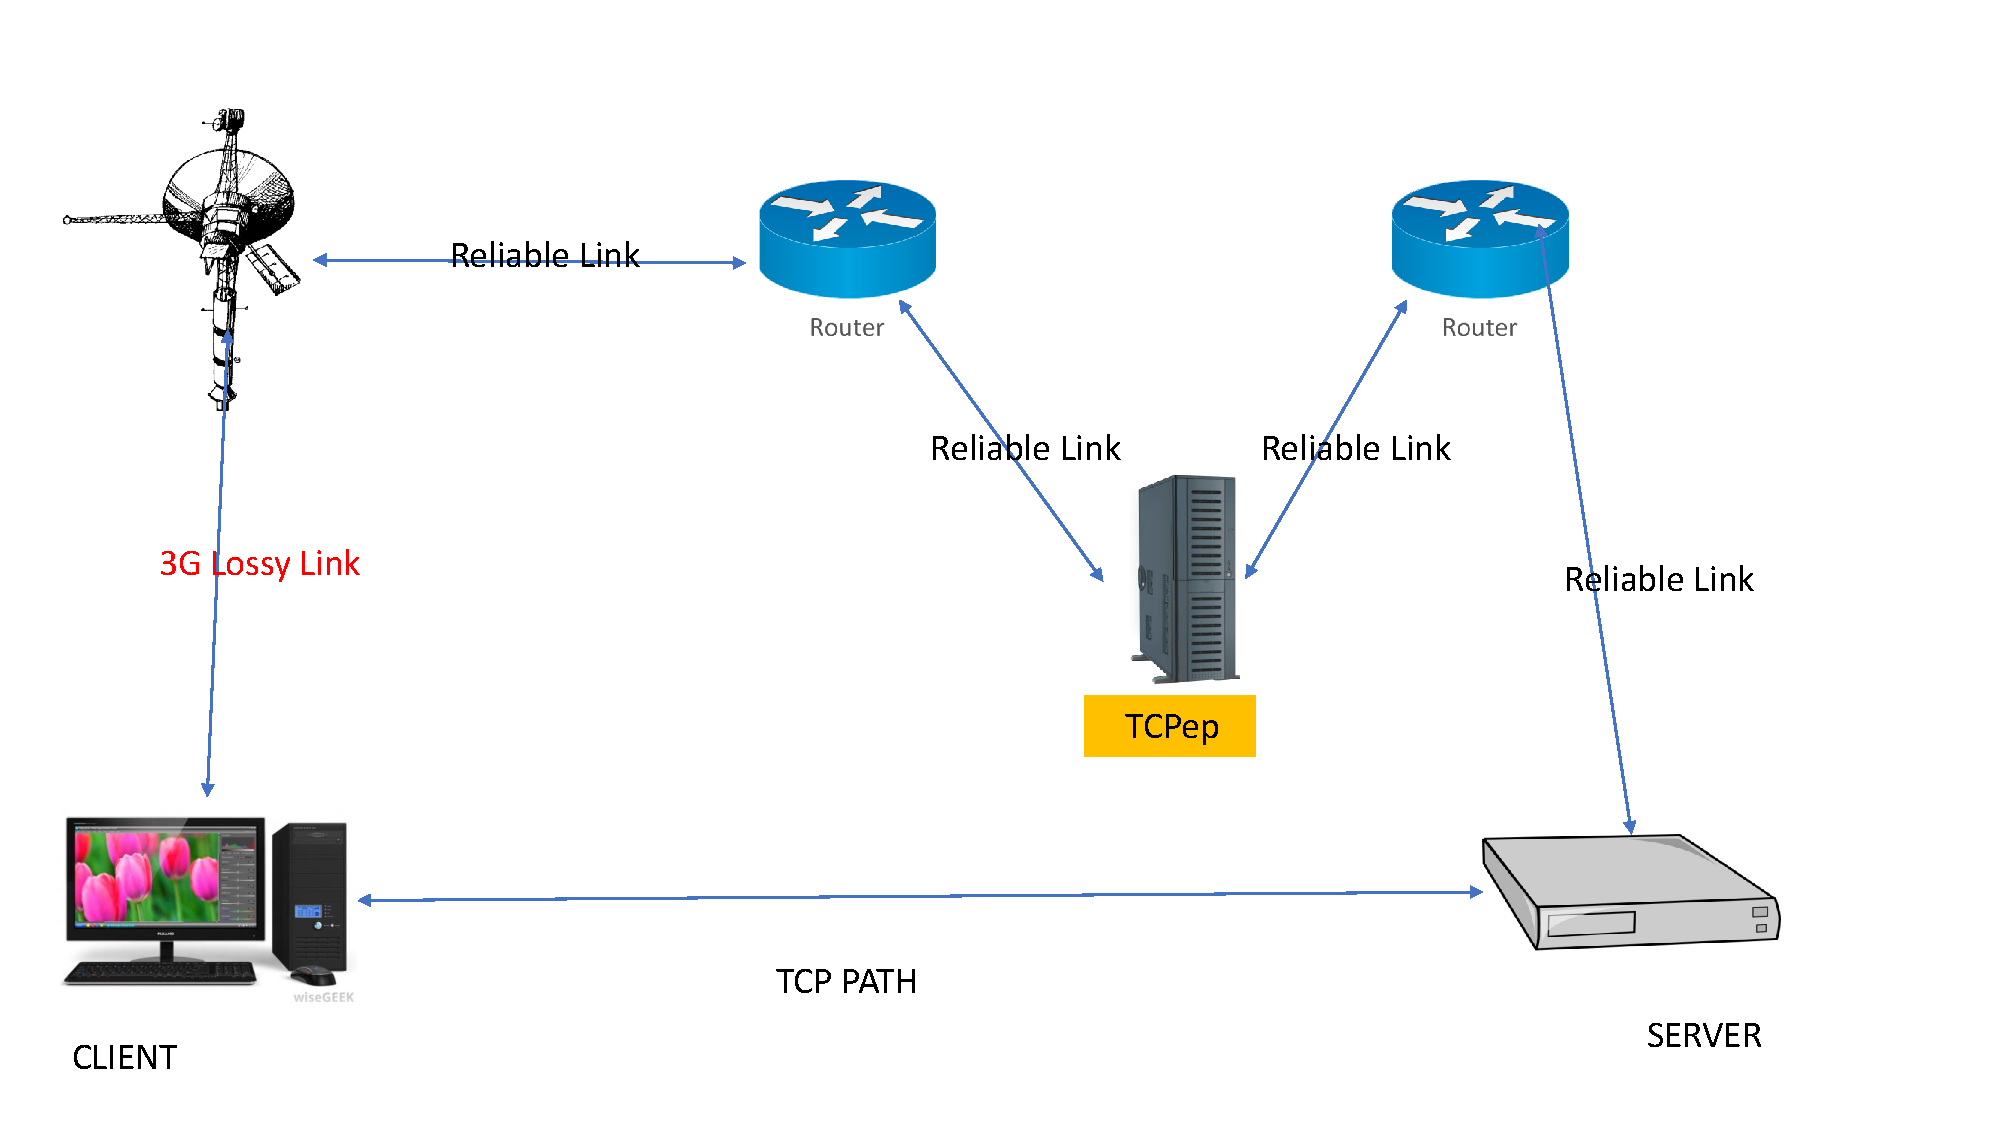
\includegraphics[width=0.9\textwidth]{TCPep.pdf}
    \caption{Typical TCPep Connection Setup}
    \label{TCPep}
\end{figure}

Therefore it was reasoned that lossy links that experience completely random losses, as has been the case in wireless links, will experience link degradation because the TCP connections are "spending excessive time in congestion avoidance and/or slow start procedures triggered by packet losses due to transmission errors" ~\cite{6}, because such losses are mistakenly treated as the result of congestion. Slow Start, for example, would assume there is congestion on the network and decrease its cwnd unnecessarily leading to undesirable results. TCPep was specifically developed to counter this type of link degradation ~\cite{33}.

TCPep makes use of network coding and an advanced algorithm to counter these effects. This thesis will not go deeply into those details as it is designed mostly for random losses on lossy links rather than queue drop losses caused by long RTT times in satellites. If the reader may wish to research more on network coding for TCPep, see section 2.2.5. 

\subsubsection*{TCPep connection type}
With TCPep, the PEP categorisation is not as important as the motivation behind its creation. We have already given an in-depth description of PEP categorisations earlier, and this one does not differ so much from the PEPsal example, so will keep it very brief here. (Differences with commercial PEPs are worth mentioning, however, so slightly more detail will be given on the categorisations when discussing commercial PEPs). 

\subsubsection*{TCPep distribution type}
TCPep is an open source integrated PEP ~\cite{33}. 

\subsubsection*{TCPep layering type}
TCPep is a transport layer PEP ~\cite{33}.

\subsubsection*{TCP splitting}
TCPep is a TCP splitting PEP ~\cite{33}.

\subsubsection*{TCPep symmetry type}
TCPep is an asymmetric PEP ~\cite{33}.

\subsubsection*{TCPep transparency type}
TCPep is transparent to the TCP hosts and end users in the network layer ~\cite{33}. 

\subsection{Commercial PEPS} 
Commercial PEPS are usually classified as proprietary "black boxes" ~\cite{6}. In other words, the network degradation protocols/solutions they use in their PEPs are not divulged to anyone in academia or the general public. PEP vendors will not necessarily be keen to submit to an academic study as they could be wary of getting unflattering results that could adversely affect sales. These vendors are also in competition with other commercial entities so it is understandable that they would want to be secretive about their methods. Any material with information on these PEPs is usually comes in the form of sales material. Naturally, one cannot expect this information to be objective and it is likely that the information presented would be overly optimistic about the effectiveness of its product ~\cite{6}. There is also the financial barrier of having to buy a commercial PEP in order to to perform an analysis on it in a study such as this. These reasons make it difficult to study commercial PEPs objectively, therefore they are beyond the scope of this thesis, but we will examine one commercial PEP (FastSAT) for the sake of an analytical comparison ~\cite{34}.\\

Unlike the previous two PEPS, commercial PEPS are costly and usually distributed (not integrated). The architecture for a typical commercial PEP can have several black box PEPs along the degraded link with modifications made to the endpoints to accommodate and maintain/enhance the throughput and reliability of the degraded network link. As Figure \ref{FastSat} shows, we have a commercial PEP called FastSAT that shows two PEPs located on both ends of the satellite link ~\cite{6}~\cite{34}. \\

FastSAT advertises "A satellite link specific, highly optimised, Flight Protocol (FP) is used for the satellite link instead of the standard TCP protocol. Alternatively, an interoperable TP protocol can also be automatically selected" ~\cite{34}. \\

In other words, it uses its own proprietary protocol tailored specifically for Satellite links and similarly degraded links affected by long RTT times. It does not, however, say exactly how its FP protocol works, what algorithm it uses etc., anywhere in its advertisement pages. The system is offered as a "black box" ~\cite{34}. \\

\subsubsection*{FastSAT distribution type}
FastSAT is a distribution type PEP, like most commercial PEPs.  As Figure 3.6 shows, FastSAT PEPs are distributed on both sides of the degraded link ~\cite{34}.

\subsubsection*{FastSAT layering type}
This FastSAT PEP operates at the Transport Layer. It replaces the TCP protocol with its own proprietary protocol FP which is designed specifically for throughput optimisation in satellite link environments. Exactly how its protocol achieves this is a trade secret, as is commonly the case with commercial PEPs ~\cite{34}. 

\subsubsection*{FASTSAT TCP splitting/protocol alteration}
FastSAT uses the TCP splitting method as does PEPsal, but it also modifies the protocol so it can be categorised under both headings. It acts as an unseen intermediary middleman between two endpoints (TCP Splitting) and deploys its own proprietary protocol FP ~\cite{34}.

\subsubsection*{FastSAT transparency type}
FastSat falls under the transparency category. As mentioned earlier, there are four degrees of transparency. Its degree of transparency is "transport layer transparency" because it is transparent with respect to the transport endpoints whom the middleware proxies are sending spoofed communications to ~\cite{34}. \\

\begin{figure}[ht!]
    \centering
    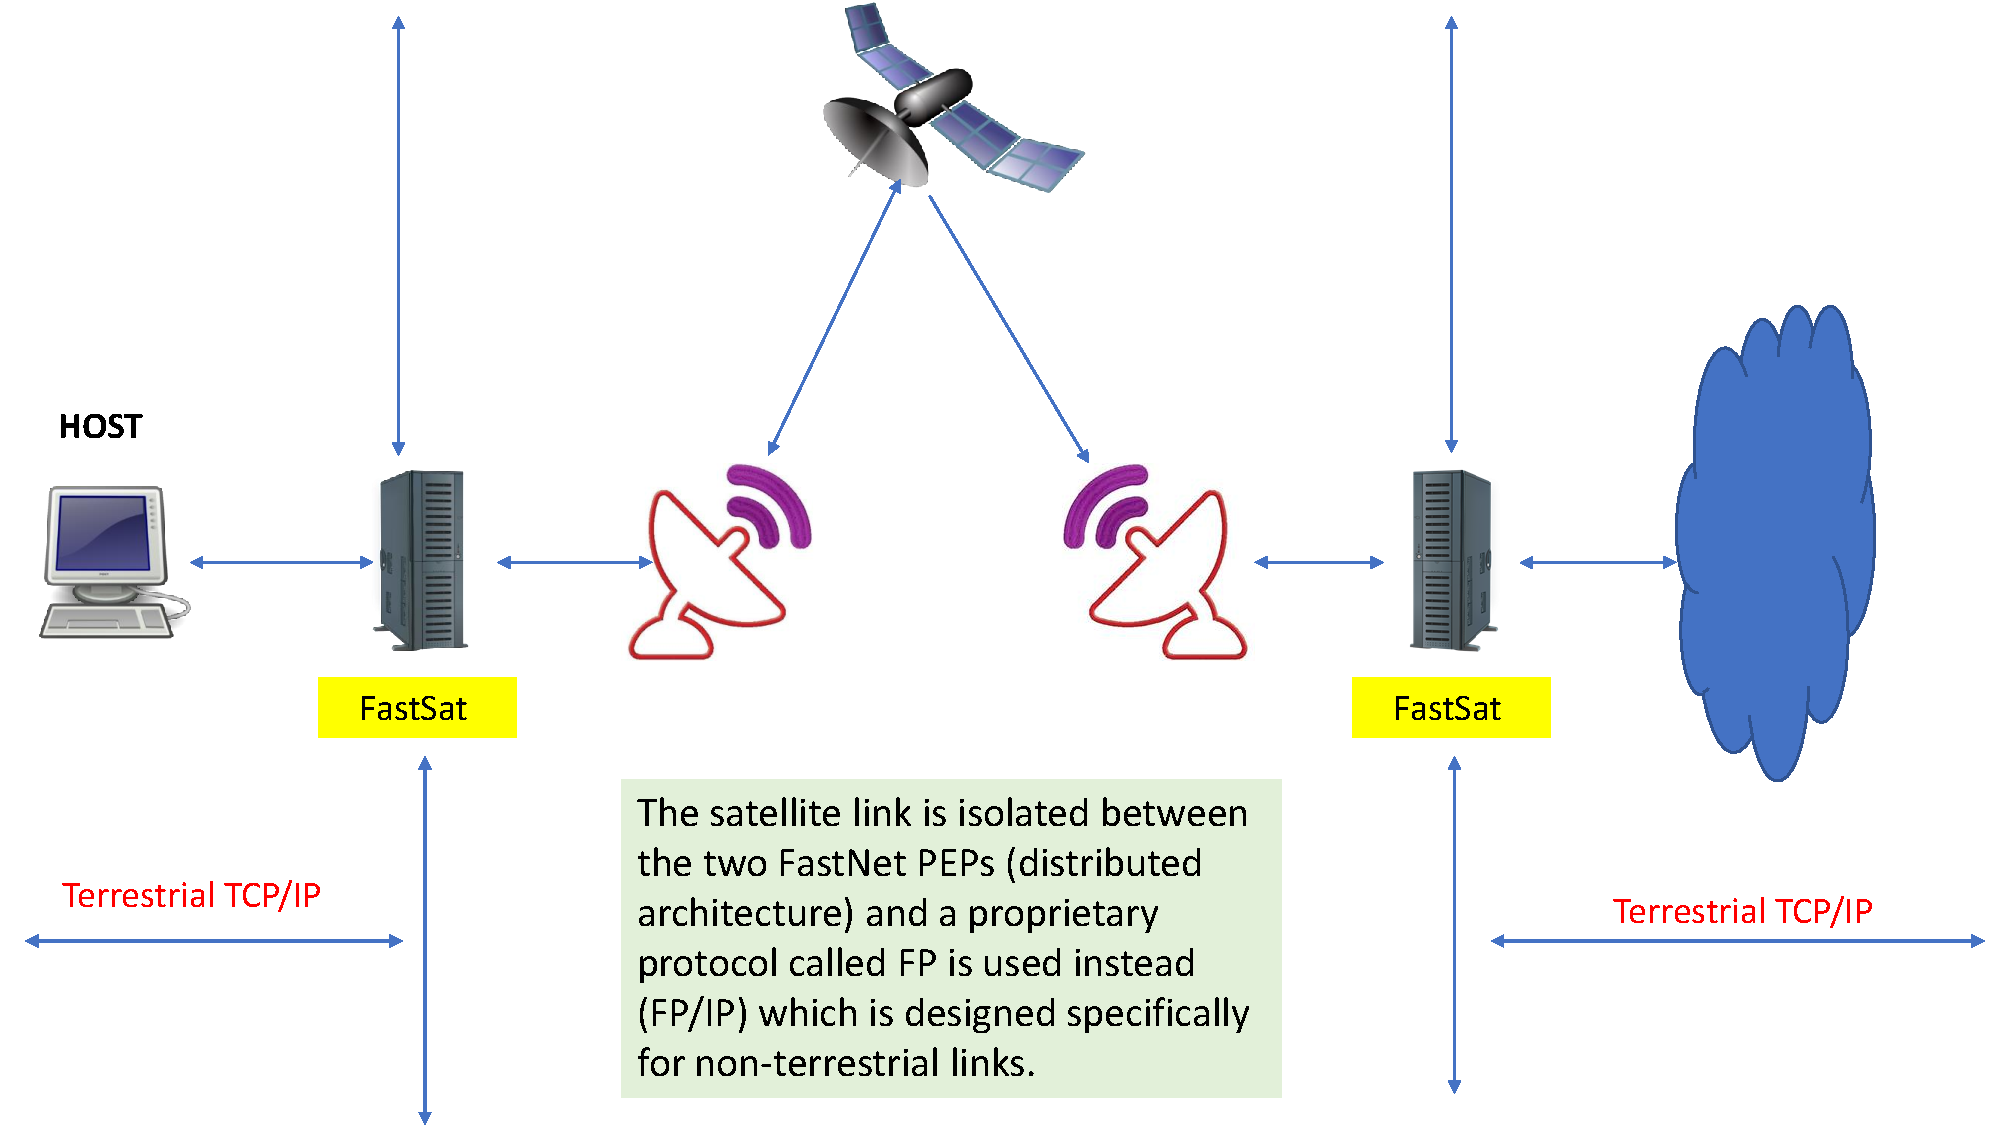
\includegraphics[width=0.9\textwidth]{FP.pdf}
    \caption{Proprietary FP Protocol}
    \label{FastSat}
\end{figure}

\subsubsection*{Summary}
In summary, this chapter has covered three different kinds of PEPs that were based on differing motivations and employing different strategies for resolving link degradations. The PEPs were also categorised according to standard RFC PEP classifications to highlight the variety of PEP functionalities and features available, but without getting bogged down in too much technical detail.  In the next chapter, details of our proposed solution takes the reader through the methods used for creating our PEP.




%chapter 4: Beacon Software Requirements
%----------------------------------------------------------------------------------------
%	CHAPTER 4
%----------------------------------------------------------------------------------------

\chapter{METHODOLOGY}

In this chapter, we show the methods we employ to create our proposed thesis solution to the long latency bottleneck satellite link problem described in previous chapters. 

\section{Socket Programming In C}
Our proposed solution to the stated research problem involves the design of a performance enhancing proxy (PEP) modified to suit the Pacific Island environment. The novelty or distinguishing facets/distinctive qualities of our PEP will be elaborated on in Section 4.3 "Our Proposed Solution", but we first start with the discussion of a few techniques that are specific to the type of programming used for standard PEP creation; namely raw socket programming. There are other languages we could have chosen to use for Socket programming (Java, Python) but we chose to use C as it is one of the few languages that properly supports raw sockets and is also the fastest once compiled. Fast processing speed is important in the satellite type environment ~\cite{35}.\\

C is ideal for firmware or portable applications. Its proximity to assembly language means that although it is considered a high-level language,  it is low level enough by comparison to modern language standards (C\#, Java, Python) to allow detailed composition, manipulation and parsing of Internet packet structures ~\cite{35}~\cite{36}. This feature is essential because to create the PEP, we must be able to spoof packets and resend them, and this will involve reading incoming packets and resetting flags and ACKs, creating our own ARP packets and more to emulate expected responses to and from two different hosts in the network. These actions require access to the IP layer, TCP transport layer and the data link layers. We will need raw socket programming for this purpose ~\cite{38}. 

\subsection{Sockets}
\begin{figure}[h!]
    \centering
    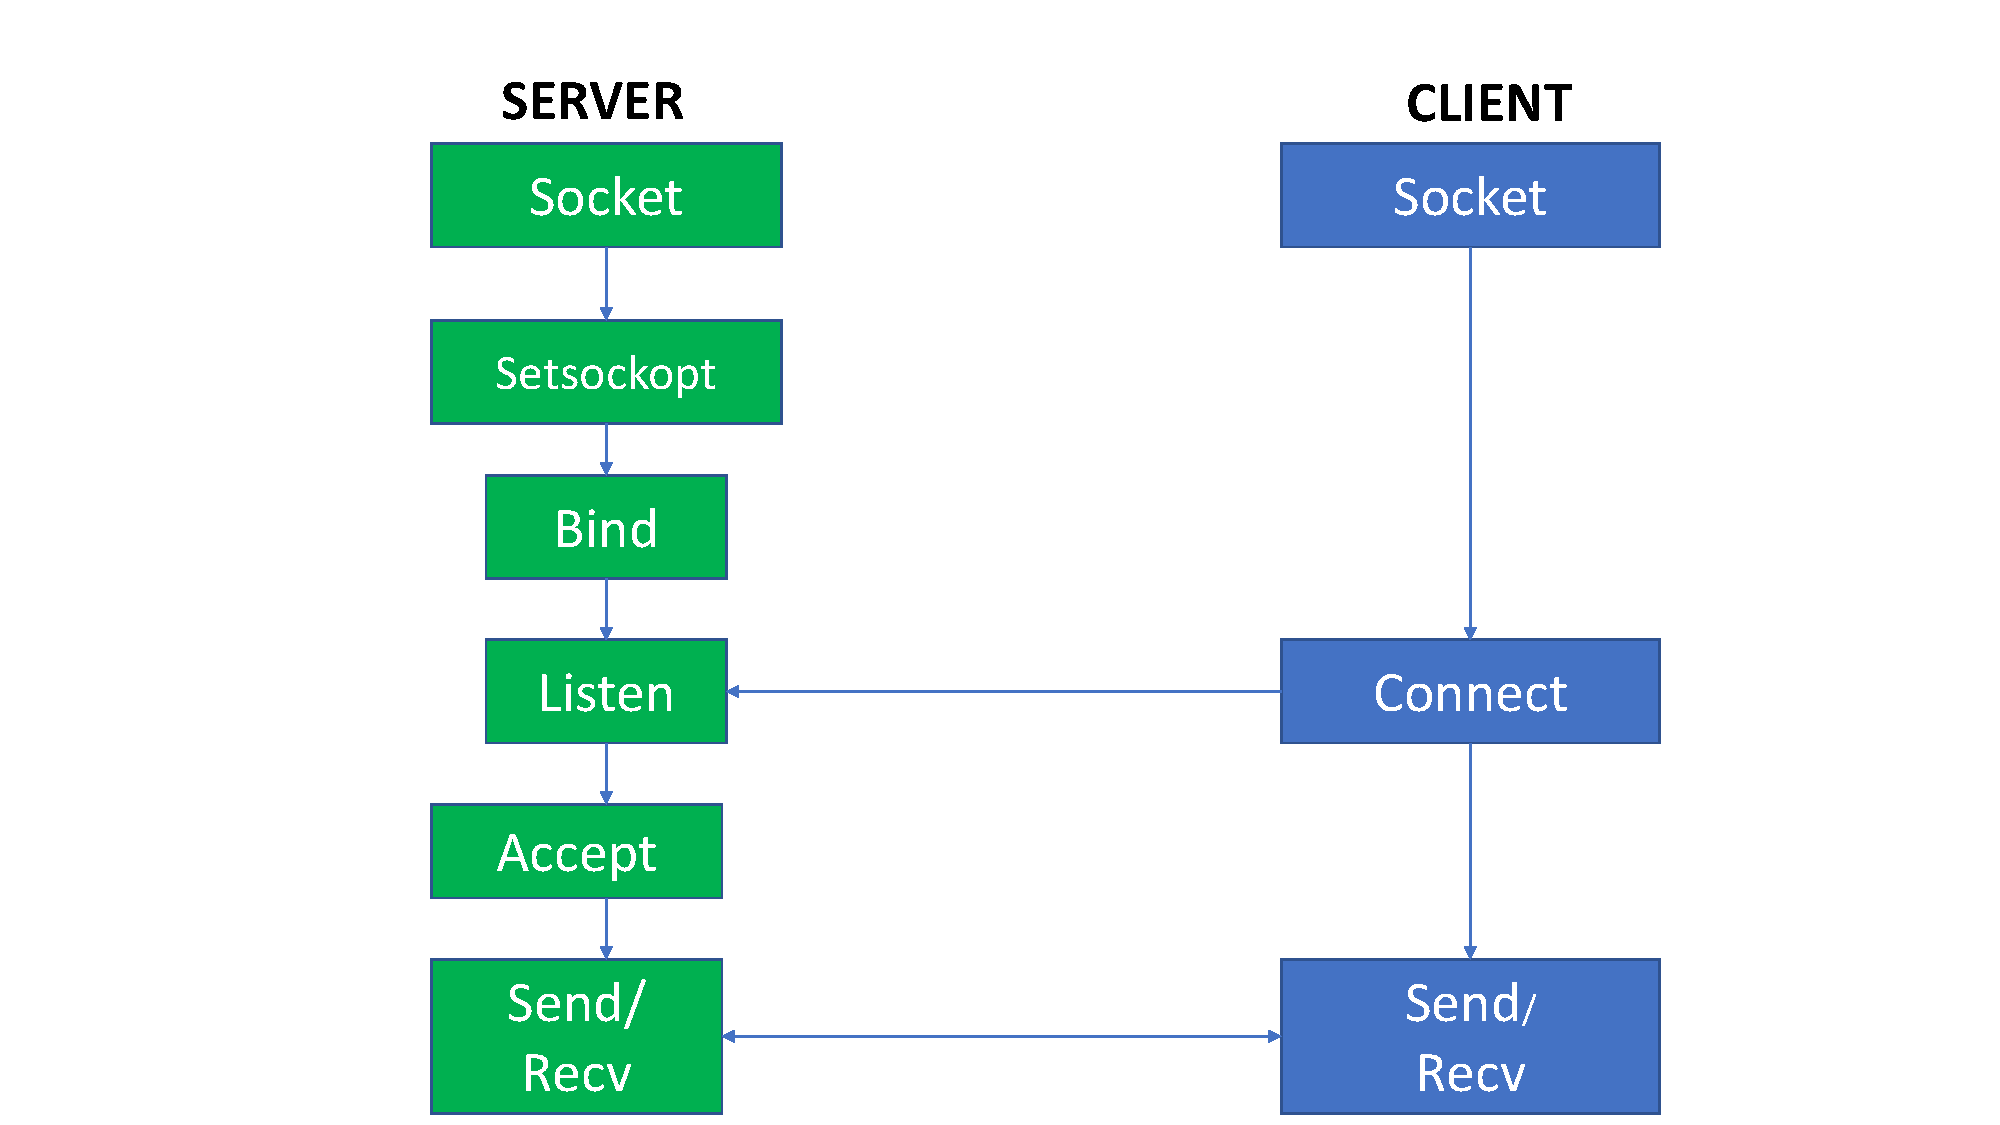
\includegraphics[width=1.2\textwidth]{ServerClient.pdf}
    \caption{Server + Client Sockets. Shows interaction between Server and Client via Sockets.}
    \label{ServerClientModel}
\end{figure}

Sockets are a key concept for this thesis. This thesis, however, will be dealing with raw sockets but to understand what raw sockets are, we must first understand what sockets are in general, of which raw sockets are a subset ~\cite{38}. In C, raw sockets are available for use at the transport layer (TCP), IP layer and data link layers. The following example described below are for the more commonly used transport layer sockets. \\

Sockets are endpoints for communication in the network infrastructure. They allow two nodes in a network to communicate with one another. Without getting too technical, the socket concept can be understood, in simple terms, using a telephone analogy. When we create the sockets via socket programming, it is analogous to installing a telephone on either end of the communication line between two parties ~\cite{37}. The telephone/socket is an endpoint between two parties/computers that enables them to establish communication. An endpoint is a unique combination of an IP address and a port number in the networking world. The telephone can be likened to an endpoint combination of a telephone number (IP address) and an extension number(port number) ~\cite{37}. \\

In the network world, the Client-Server model is the basis for most communication. The Server is always listening for a client to connect. Once a client connects after connection handshake, it can request information. The Server serves this information to the client and the client disconnects (the server can also disconnect). The Server will be on standby again to listen for more connections from clients ~\cite{35}. \\

We can create sockets using a few "function calls" or set of programming requests from the socket application programming interface/ socket API. In keeping with the telephone analogy, here are a few of the key code calls used in socket programming in C ~\cite{35}~\cite{36}.
   \begin{itemize}
   \item Socket() -Endpoint for communication/ create telephone on either end:\\
   int socket = socket(domain, type, protocol)
   \item Bind()- Assign a unique IP address and specific port number/ telephone number to distinguish this endpoint from other endpoints on the network:\\
   int bind(int socket, const struct sockaddr *addr, 
                          socklen\textunderscore t addrlen);
   \item Listen()- Listen for an incoming connection/ wait/be ready for an incoming call:\\
   int listen(int socket, int backlog);
   \item Connect() -request connection to another endpoint/ dial a phone number:\\
   int connect(int socket, const struct sockaddr *addr,  
                             socklen\textunderscore t addrlen);
   \item Accept() -accept incoming connection request/ receive a phone call, i.e. answer the phone:\\
   int new\textunderscore socket= accept(int socket, struct sockaddr *addr, socklen\textunderscore t *addrlen);
   \item Send(), Recv()- exchange data over the established connection/ talk over the phone to the other person: \\
   ssize\textunderscore t send(int socket, const void *buf, size\textunderscore t len, int flags);
   ssize\textunderscore t recv(int socket, void *buf, size\textunderscore t len, int flags);
   \item Close()- Terminate connection and endpoints/ hang up the call once talking is done. \\
   int close(int socket);
   \end{itemize} 
   
\noindent \emph{Note: The calls to pay most attention to here for future reference are {\tt Socket(), Bind(), Send()} and {\tt Recv()} as they will be used again in raw socket programming for the PEP.} 

\subsubsection{Regular TCP sockets vs raw sockets}
Regular socket programming operates on the transport layer protocol. It deals with TCP and UDP transmission taking in byte stream data as input to form TCP segments. Regular TCP sockets take care of encapsulating TCP segments (including TCP headers, checksums etc.) in IP datagrams (including IP headers and header checksums) but do not alter or touch the contents of the packets which are handled by the kernel operating system. Hence the following operations are also automatically handled in regular TCP sockets ~\cite{35}:\\

\begin{itemize}
\item Ensures ACKs, retransmission, flow control, congestion control for TCP, datagrams etc.
\item Ensures encapsulation of IP datagrams into physical layer frames (typically Ethernet) including frame headers and checksums.
\item Ensures reassembly of IP datagrams from frames + fragments
\item Extraction of TCP segments
\item Ensures completeness of byte stream from TCP segments
\item outputs byte stream \\
\end{itemize}

Essentially, automatic encapsulation of the packets with the protocol headers (UDP or TCP) occurs, and the socket-user does not deal with these headers at all. With Raw Sockets, many of these operations mentioned are not handled automatically and must be programmed manually. Raw sockets are aware of the packet headers in that they receive \emph{raw packets} that can include IP headers and/or Ethernet headers depending on whether we are using a network layer or data link layer raw socket. The raw sockets can opt to include or exclude the headers upon transmission. Raw sockets bypasses the standard stack traversal and reaches down into the network and data-link layers to allow us to alter the content of these packet headers ~\cite{35}~\cite{38}.\\

This concludes the general overview, in layman's terms, of what sockets are, their purpose, and how they function.  We are now ready to proceed with explaining the concept of raw sockets in more detail and how it relates to this thesis.\\

\section{Raw Socket Programming}
Raw Sockets enable us to deliver a raw packet directly to an application without it traversing through the stack of network layers (See Figure 4.5).
In other words, we can circumvent the usual TCP/IP protocols, and this enables us to create a packet sniffer and packet injector to modify packets as per requirements for our specialised PEP ~\cite{38}. \\

\textbf{Raw sockets allow the following:}\\

\begin{enumerate}
\item Inject IP packets directly into Ethernet frames (but let the kernel take care of Ethernet frame assembly) and send them.
\item Assemble and send entire Ethernet frames
\item Receive Ethernet frames/IP packets individually regardless of protocol\\
\end{enumerate}

The network stack removes all headers from packets as they move up the stack, transporting only the data to the application layer. (See Fig 4.3). Conversely, data sent from the application layer back the other way has headers added as it traverses down the stack. So whilst other sockets only interact with the transport layer and deal exclusively with payload data, raw sockets take packets from the Ethernet layer(raw packets) complete with headers and can forward them directly to the intended application. If a communication flow is occurring between different processes in regular sockets, then these processes are only exchanging data ~\cite{38}.\\

Raw packets, defined as a packet with headers included, have the source IP address and MAC address information loaded into their headers, and this is crucial information needed to construct our PEP. Our PEP must be able to spoof packet header information in outgoing packets header and forward them to the intended hosts. For this purpose, it must also be able to read IP/TCP headerand Ethernet header information. The next section will detail how we use raw socket programming to build our PEP starting with a fundamental building block for all PEPS: \emph{The packet sniffer} ~\cite{38}.\\

\begin{figure}[h!]
    \centering
    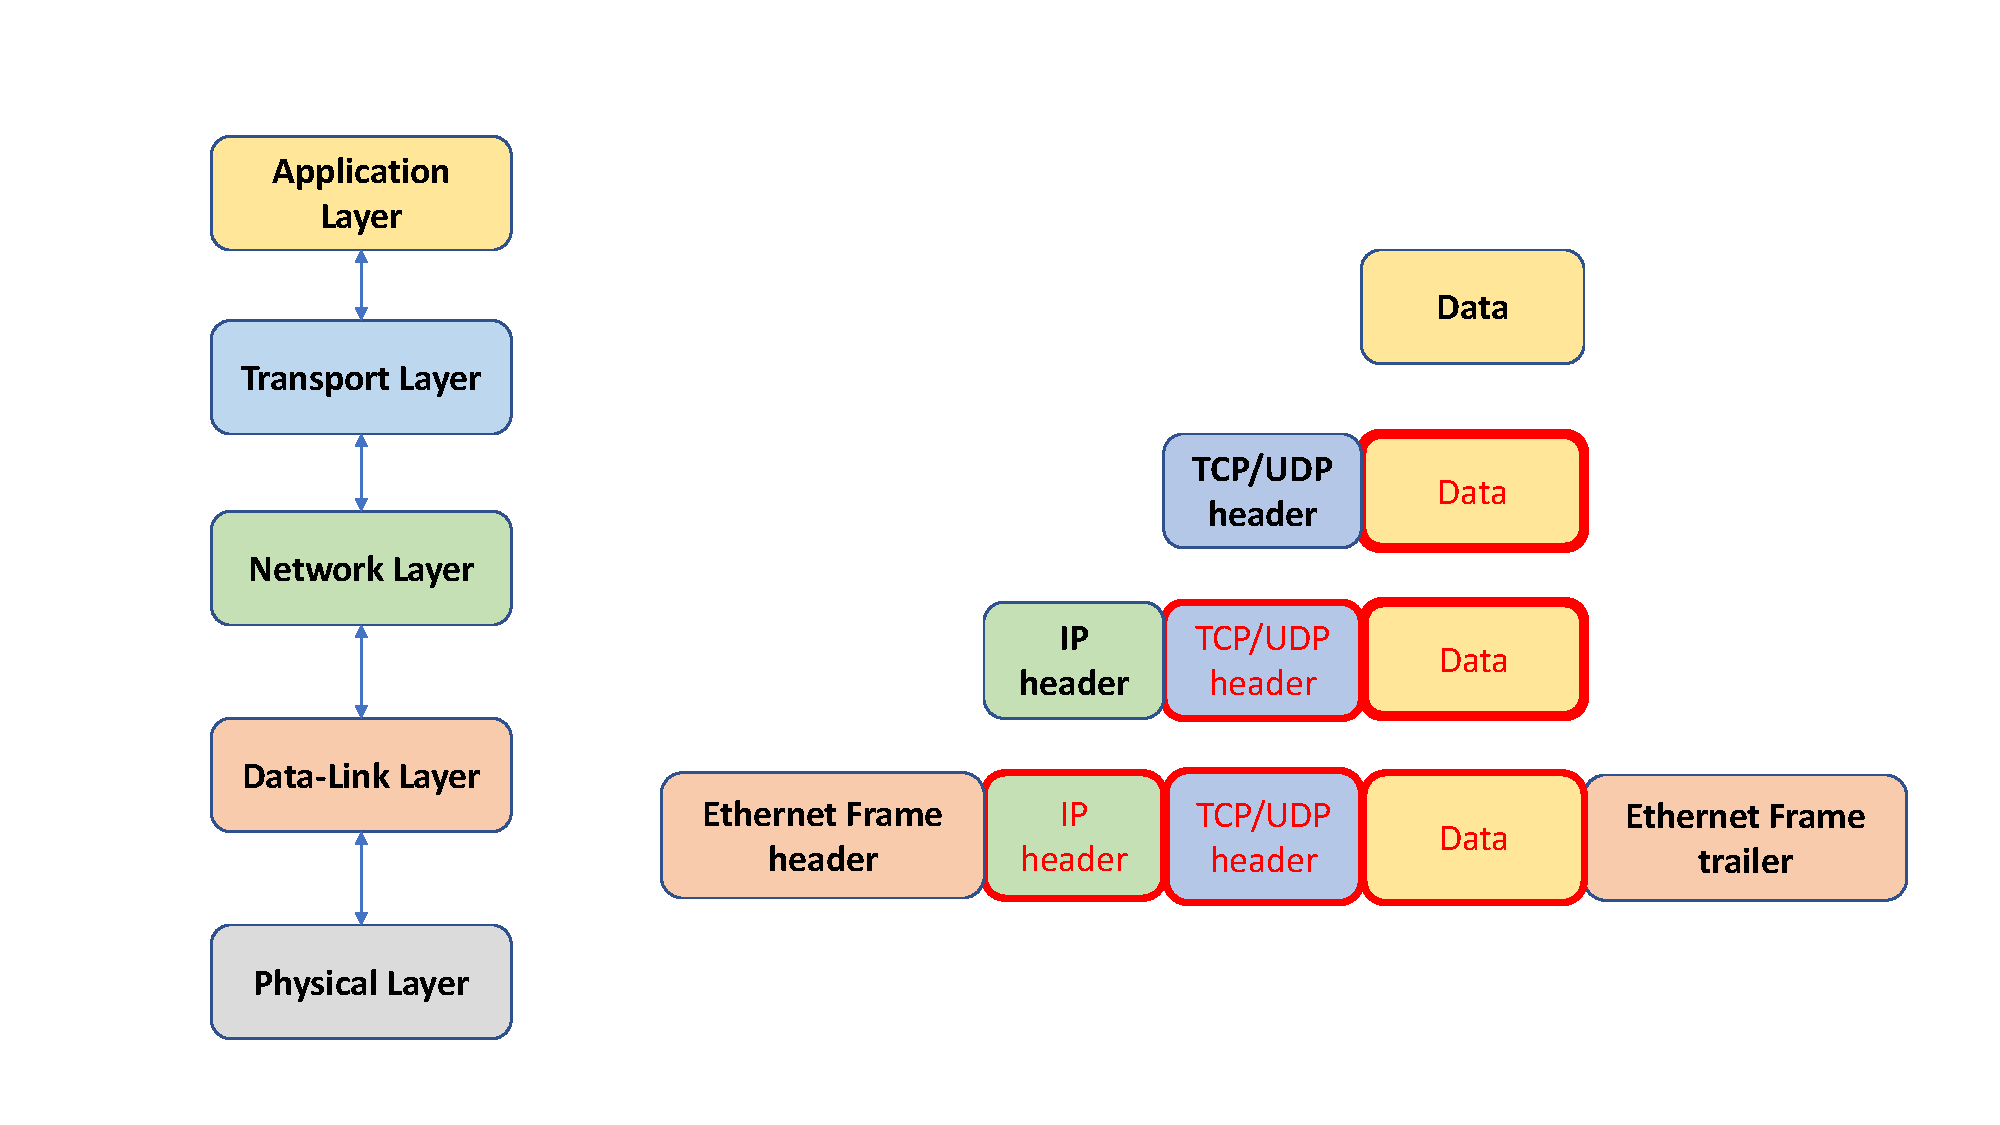
\includegraphics[width=0.95\textwidth]{NetworkTraversal.pdf}
    \caption{Headers being stripped + added during Network Stack Traversal
    }
    \label{fig:Socket}
\end{figure}

\subsection{Creating a packet sniffer}
To build a PEP that can forward packets and that can act as a proxy that can emulate ACKs for incoming packets, we need to be able to intercept and fully interpret these packets. The PEP must be able to see all the information in the headers as well as the data payload. This requires the creation of a packet sniffer as the first step to achieving our PEP ~\cite{38}. \\

We are using a Linux system for experiments in the lab. Linux has its own packet sniffer tool called \textbf{tcpdump} ~\cite{35}, but for this thesis we created our own packet sniffer with C programming. This provides one of the building blocks for our non-connection breaking PEP. \\

\textbf{To create a packet sniffer, we first need to create a raw socket:} \\

The packet sniffer is created by: 
    \begin{itemize}
        \item Using raw socket call to create a socket object- \\
        {\tt int socket= socket(int socket\textunderscore family, int socket\textunderscore type, int protocol);}\\
{\tt \textbf{rawSocket = socket(\textcolor{blue}{AF\textunderscore INET}, \textcolor{purple}{SOCK\textunderscore RAW} , \textcolor{orange}{IPPROTO\textunderscore TCP});}}
        \item Make sure interface is set to promiscuous mode for packet sniffing. Allows us to receive all packets, not just packets bound for the machine attached to the interface- use {\tt ioctl()} or use infinite while loop with {\tt recv()} (See Figure 4.4 for an example).
        
        \item Bind Raw Socket to the interface we want to listen to-use {\tt bind()}\\
{\tt int bind(int socket, const struct sockaddr *addr, socklen\textunderscore t addrlen);}\\
{\tt \textbf{bind(sd, (\textcolor{purple}{struct sockaddr *}) \&sll, \textcolor{blue}{sizeof}(sll))) == -1)}}
\item Receive packets on the socket using recv()\\
{\tt recv(int sockfd, void *buf, size\textunderscore t len, int flags);}\\
{ \tt \textbf{recv(rawSocket, buffer,\textcolor{blue}{65536}, 0)}}

        \item Close the raw socket() -never reaches this point if on infinite while loop\\
        int close(int rawSocket);\\
    \end{itemize}
    
The packet sniffer will set the interface to promiscuous mode so that it receives frames for all hosts in its broadcast domain irrespective of whom they are addressed to. Simply put, the sniffer allows eavesdropping on all packets observed on the same physical network ~\cite{35}~\cite{38}.\\

The sniffer will receive raw packets, complete with TCP, IP and Ethernet headers, or ARP headers, ICMP headers etc., for example, which we will be able to analyse and manipulate via our PEP. The next step component for the PEP is the capability to inject packets into the network. Once our PEP has analysed the sniffed packet and extracted the data, we can manufacture our own spoofed packets with custom-made headers and data payload for forwarding ~\cite{38}.\\

\subsection{Creating a packet injector}
Another essential element in the creation of our PEP is the ability to forward incoming packets the PEP receives.  
The creation of the packet injector is similar to that of the set up for a packet sniffer ~\cite{35}~\cite{38}.  \\

\textbf{For packet injector-}\\
    \begin{itemize}
        \item Using raw socket call to create a socket -socket()
        \item Bind Raw Socket to the interface we want to send packets on-use bind() or setsockopt()
        \item Create a new packet using info extracted from the sniffed packet
        \item Send the packet -sendto() transmits the packet to another socket \\
sendto(int socket, const void *buf, size\textunderscore t len, int flags,
               const struct sockaddr *dest\textunderscore addr, socklen\textunderscore t addrlen);        
        \item Close the raw socket()\\
    \end{itemize}

\begin{figure}[h!]
    \centering
    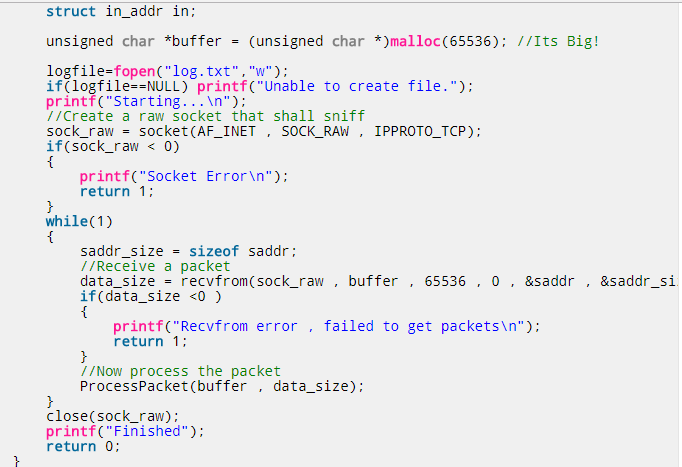
\includegraphics[width=0.87\textwidth]{SnifferCode.PNG}
    \caption{Example of basic sniffer code in Cl
    }
    \label{fig:Sniffer code in C}
\end{figure}

The sample code in Fig 4.4 shows the basic setup for a sniffer. We see the socket () call taking three parameters, int domain, int type and int protocol which returns an int that represents a socket file handle of the operating system ~\cite{35}~\cite{38}. \\

The \textbf{domain} here is AF\textunderscore NET which stands for "Address Family", and this allows for IP addresses specifically. 
A socket address in the AF\textunderscore INET family contains four fields: 

\begin{enumerate}
     \item The name of the address family itself (AF\textunderscore INET).
     \item The IP address (Ipv4).
     \item The port number.
     \item The reserved field of 8 bytes ~\cite{36}. \\
\end{enumerate}

The \textbf{type} specifies the type of socket we want to open. For regular socket programming, we want to open either a SOCK\textunderscore STREAM for a TCP socket or SOCK \textunderscore DGRAM for a UDP socket. For the packet sniffer, we require a raw socket that receives full packets (raw packets) with header information (Source IP, Source MAC address etc.) included, so we use the constant parameter SOCK \textunderscore RAW as  \textbf{type} ~\cite{36}~\cite{38}. \\

Lastly, we have the \textbf{protocol} parameter which is set to IPPROTO\textunderscore TCP in the code snippet (Figure 4.4) which sets up the sniffer to receive raw TCP packets. Usually, only one protocol exists within a socket so it can be set to 0 but in some cases, there is more than one, so the need to specify a protocol is required ~\cite{35}.\\

\begin{figure}[h!]
    \centering
    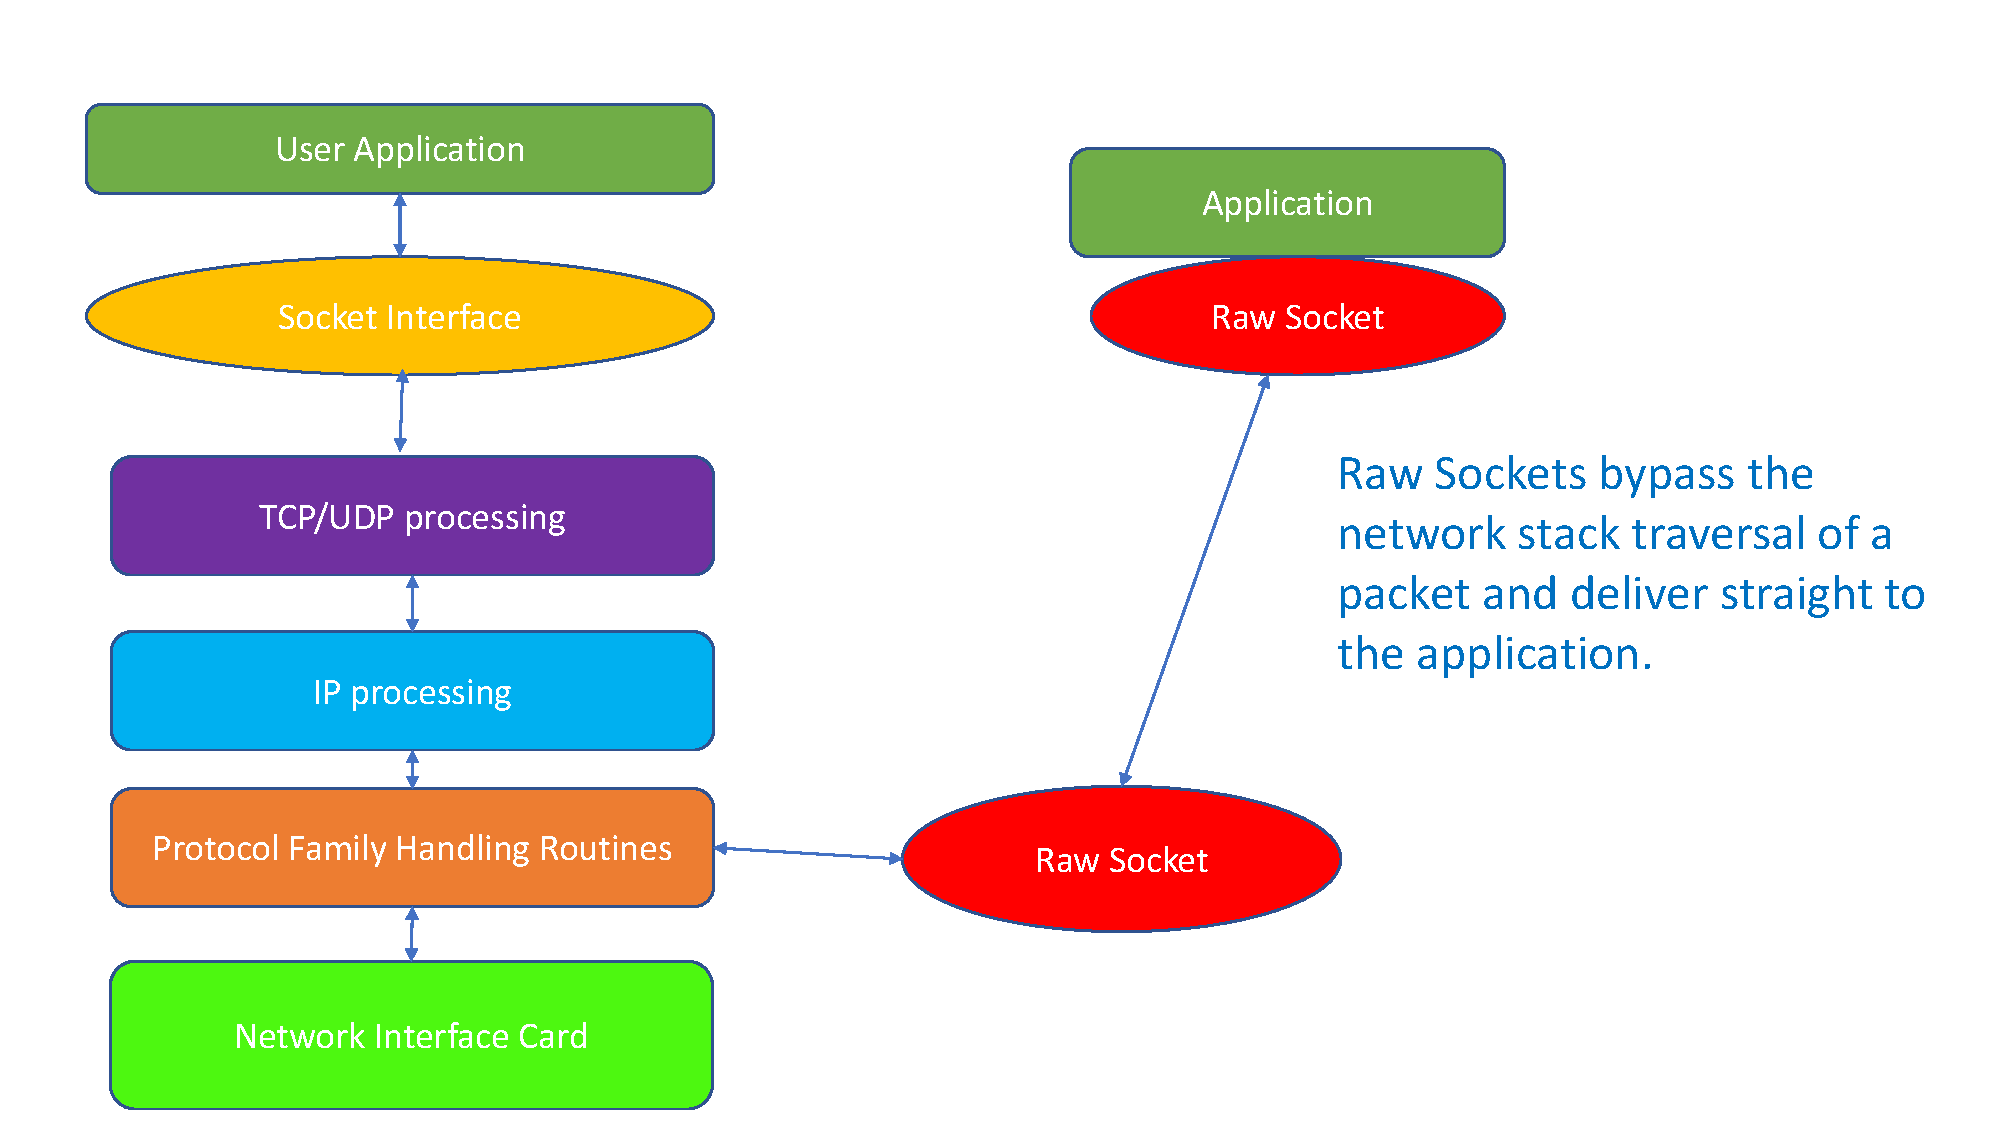
\includegraphics[width=0.95\textwidth]{stackTraversal.pdf}
    \caption{Raw Socket Bypassing Kernel Stack Traversal}
    \label{RawSocketTraversal}
\end{figure}

We also have IPPROTO\textunderscore IP, if used in conjunction with socket type SOCK\textunderscore STREAM and AF\textunderscore NET, causes the kernel to set the protocol to TCP automatically (as if using IPPROTO\textunderscore TCP). \\

The same, however, will not work when these two parameters are used with SOCK\textunderscore RAW. The SOCK\textunderscore RAW must be used with the correct protocol which can only be called explicitly ~\cite{36}~\cite{38}.\\

In our sniffer, we set the protocol to IPPROTO\textunderscore RAW as we want to interact directly with the lower layers 3 (network layer) and layer 2 (data-link layer/Ethernet). The prepending of headers is usually handled by the kernel, but we want to execute packet injections from our PEP and edit the headers and payloads ourselves. This gives us the flexibility needed to spoof packets and override any default information from the kernel by bypassing the usual stack traversal processes altogether (see Fig. 4.5) ~\cite{38}.\\

\subsection{Binding sniffer to an interface}
The next step is to bind that sniffer to an interface we want to listen to. Binding the sniffer to a particular interface ensures that the sniffer only listens for packets on the bound interface, rather than on every interface. \\

To do this, we need to extract the interfaces kernel identification number or file handle using standard \emph{ioctl} calls which we will explain in more detail later. \todo{promise}Since we are coding this in C; we are dealing with structs (See Section 2.2.5 - Other Concepts Used In This Thesis). \\

We can liken structs to classes in Java complete with fields or attributes but excluding methods ~\cite{39}. The sniffer code will use structs to store the information needed for various operations. This thesis will not delve into structs in too much detail. Although structs are a concept of C programming that is used here, understanding the struct concept and how it is used to create our PEP is sufficient ~\cite{39}. As can be seen in the struct ifreq below, we see a struct that looks like a class with attribute fields. Structs ifreq in the code snippet 4.6 is declared as struct ifreq {\tt ifr} with {\tt ifr} being a variable of type struct ifreq. \\

Take note of the fields in the struct ifreq below and the caption in figure 4.6 explaining the code attached to the ioctl call. The ioctl call in figure 4.6 will look at the interface name that is stored in the {\tt ifr\textunderscore name} field and returns the interface index number and stores it in the {\tt ifr\textunderscore index} field. \\

\lstset{language=C,
                basicstyle=\ttfamily,
                keywordstyle=\color{blue}\ttfamily,
                stringstyle=\color{red}\ttfamily,
                commentstyle=\color{green}\ttfamily,
                morecomment=[l][\color{magenta}]{\#}
}

\begin{lstlisting}
struct ifreq { 
    char ifr_name[IFNAMSIZ]; // Interface name
    union {
        struct sockaddr ifr_addr;
        struct sockaddr_ifr_dstaddr; 
        struct sockaddr ifr_broadaddr;
        struct sockaddr ifr_netmask;
        struct sockaddr ifr_hwaddr;
        short ifr_flags;
        int index;
        int ifr_metric;
        int ifr_mtu;
        struct ifr_map;
        char ifr_index;
        char sockaddr ifr_metric;
        char sockaddr ifr_mtu;
    };
};
\end{lstlisting}

\begin{figure}[h!] 
    \centering
    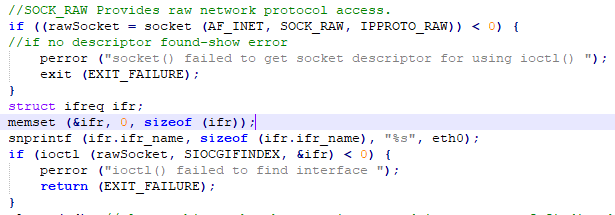
\includegraphics[width=0.9\textwidth]{Struct_ifreq.PNG}
    \caption{IOCTL call to find interface kernel index. ifreq struct {\tt ifr} has been nulled out by memset. The snprintf stores the name of the chosen interface as a string in the {\tt ifr} name field. Next the ioctl takes a rawsocket as its first parameter, uses it to carry out the instruction in the second parameter (SIOGIFINDINDEX) to find the kernel index of the interface name stored in {\tt ifr} name field. Finally, on successful completion, The index number is stored the {\tt ifr} index field}
    \label{fig: http://man7.org/linux/man-pages/man7/netdevice.7.html}
\end{figure}

\subsubsection*{Struct Ifreq:}
For our lab's Linux based systems, we can use a struct ifreq to pass data received via an ioctl call as seen in line 3 of Fig 4.6 {\tt "ioctl(rawSocket, SIOCGIFINDEX, \&ifr)"}. Linux makes use of standard ioctl calls for configuration of network devices ~\cite{40}. They can be utilised in conjunction with any socket file descriptor to retrieve information about the network (e.g. interface name, interface index, interface MAC address etc.). The ioctl call will find the interface name that is stored in the ifreq struct {\tt ifr} and can extract any of the attribute information contained in its struct fields (in this case, we want interface index number as catalogued by the kernel so we can use it later to bind our socket sniffer to that interface). The struct ifreq allows a programmer to get and set network configurations ~\cite{40}. \\

In Fig 4.6, ioctl takes three parameters. The first parameter named rawSocket, is a raw socket we create specifically to find the kernel index number for this interface. (Line 1 of Fig 4.6, opens a raw socket). The second parameter is an instruction for the ioctl to perform. In this case, the instruction is to populate the if\textunderscore index field of the ifreq struct using the interface name we stored in the ifreq struct variable ifr. The third parameter is where the socket stores the found kernel index. More specifically, it is the memory address of the corresponding ifreq struct field containing a kernel index ~\cite{35}~\cite{40}. \\

This struct is used frequently throughout this thesis because of its ability to store all the information needed for our packet injector (i.e. interface index number, interface IP address, interface netmask etc). it will have any of its fields populated depending on the instruction given as a second parameter ~\cite{35}~\cite{40}. This will be of use again when the next hop interface MAC address and index are required to forward packets on for our packet injector. This will be discussed in more detail in Section 4.2.4 "Forwarding Packets".\\
 
In Figure 4.7, the {\tt bind()} call will bind the desired interface for "sniffing" via its kernel index number, which we stored earlier in the ifreq struct, to a raw socket ~\cite{35}~\cite{40}. Now the important thing to note is that any packets that pass through this interface will be heard by our sniffer. \\

\emph{As a side note, notice that we are also casting the struct ifreq {\tt ifr} to a struct sockaddr pointer as this is the type of parameter a bind call requires. When it comes to sockets, there is an absolute zoo of data types, most of which map onto each other and are partially identical internally so often we can handle them interchangeably as long as we are casting to the correct data type that a particular function requires} ~\cite{35}~\cite{39}~\cite{40}.  \\

\begin{figure}[h!]
    \centering
    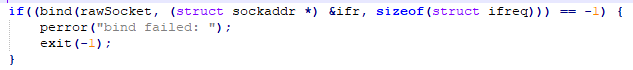
\includegraphics[width=0.9\textwidth]{Bind.PNG}
    \caption{Binding our socket to the interface we want to listen on. }
    \label{fig: Raw Socket Traversal}
\end{figure}

We can now code an infinite loop in C that will allow us to receive sniffed raw packets that have travelled past our raw socket bound interface. This infinite loop will also be the basic loop in our proxy that receives packets from incoming sockets and decides on what action to take with them. To do this, we need to use the {\tt recv()} call which receives messages from sockets and store it into a buffer. The {\tt recv()} takes 4 parameters as such; \\
{\tt \textcolor{red}{ssize\textunderscore t\ recv}\textcolor{blue}{(int sockfd, void *buf, size\textunderscore t len, int flags};}\\


\begin{figure}[h!]
    \centering
    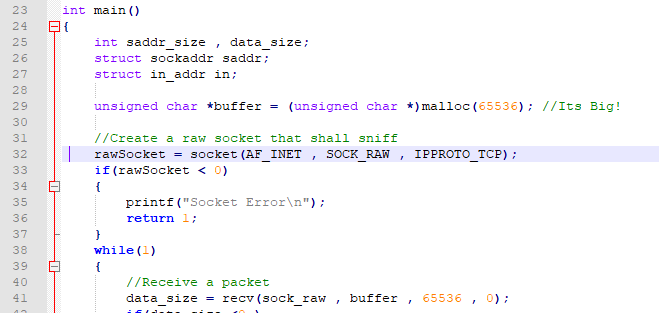
\includegraphics[width=0.9\textwidth]{InfiniteSniff.PNG}
    \caption{Infinite while loop and recv() to sniff packets}
    \label{fig: Recv} 
\end{figure}
                 
From Fig: 4.8, {\tt recv()} is reading from the raw socket we have aptly named {\tt rawSocket} which we have bound to the desired interface previously. Note that the int socket is a file handle as catalogued by the kernel. We have, at this stage, already configured the socket with all the necessary functionality for packet sniffing on an interface. The second parameter is a void pointer to a variable aptly named {\tt buffer} where we will store the incoming packet. The third parameter is the maximum size of this buffer, for which we have allocated memory from the heap via {\tt malloc()}. We use {\tt memset()} to clear the buffer memory to 0, so we have a fresh, clean slate to copy our packets to ~\cite{39}. \\


{\tt \textcolor{red}{// Set up sniffer for incoming packet}\\     
   \textcolor{blue}{unsigned char *buffer = (unsigned char *)} \textbf{malloc}\textcolor{blue}{(65536);} \\
   \textcolor{blue}{memset} \textbf{(buffer, 0, 65536)};} \\
   
The {\tt int flags} (parameter 4) is set to 0.  This sets us up for the next section where we forward packets and begin to send spoofed packets. 

\subsection{Forwarding packets}
Note that for this thesis, we are primarily concerned with the capture and duplication of TCP connection-oriented packets. Once we have established that our sniffer has bound to the desired interface and receives packets, we can start forwarding packets. The task to perform now is to ensure that we can take in an IP packet from our sniffer bound interface and forward it out on another outgoing interface with a new Ethernet header to its destination ~\cite{35}~\cite{38}. A breakdown of the steps is follows:\\

\begin{enumerate}
\item Extract the relevant information from the packet, including header information (source IP address, flags set, checksum) and the data payload. \\
\item Using a library of header structs for IP, TCP  headers to store all the information gleaned from the sniffed raw packets. \\
\item Create new Ethernet packet and forward with a copy of the original packet in it to the intended destination. We do this by allocating memory from a new buffer and utilise the header structs to set the correct fields in the correct places in the buffer. Then pass completed buffer to raw sockets {\tt send()} function.\\
\item Send ACK back to the source to acknowledge reception of the packet with the modified sequence number. \\
\end{enumerate}

We have already briefly explained how the {\tt struct ifreq} was used to extract information from an interface to be used in our raw socket binding. The concept here is the same for step 1 and step 2 where we extract header information. Step 3 also involves another substep of determining the next hop MAC address ~\cite{40}. Unfortunately, in C there is no direct programmatic in-process access to the kernel ARP table. So we have two choices at this point. We could either:\\

\begin{itemize}
\item query the kernel ARP table by starting an additional process which is restrictive if we are trying to process hundreds of packets per second. 
\item build our own ARP table and send our own ARP requests and read ARP replies that are received back.\\
\end{itemize}

We choose the second option. This involves creating our own ARP table cache, creating and sending an ARP request and waiting for the corresponding ARP reply containing the next hop MAC address needed before we can forward a packet. Any data packets (not an ARP reply or response) received will have a source MAC, source IP, destination MAC and destination IP. The destination MAC will be our incoming interface MAC address. The source MAC will be the last hop MAC just before our incoming interface MAC address in the forwarding chain ~\cite{1}~\cite{2}. To forward the packet onwards via our outgoing interface, we must fill in the destination MAC ourselves by either querying our cache table for a MAC entry for the packet's destination IP address or by using the ARP request. We will delve into that in more detail later in Section 4.2.5 "Finding the MAC address for forwarding packets". \\

In the context of forwarding, we could have also used the standard Linux packet forwarding/routing mechanisms. For this thesis, we will construct our own forwarding mechanism with C code ~\cite{39}. The advantages of building our own here is that we get: \\

\begin{itemize}
\item Access to the headers which allows us to eventually rewrite fields such as, for example, the advertised windows.
\item It allows us to decide which packets to forward and which ones we do not want to forward. 
\item It allows us to inject our own packets which we did not receive but have created ourselves (e.g. ACKs)
\item It allows us to cache packets we have forwarded until we receive ACK back from the destination \\
\end{itemize}

As is the standard with any PEP, we will receive the raw packets complete with headers. AS a consideration for future work, We will eventually be able to change the header contents and size of the advertised window to control the flow of traffic so that if there is congestion, we can limit the number of packets sent. If the link is not at capacity, we can make the window bigger to allow more packets through. We will elaborate on this further in Section 4.3 "Our Proposed Solution". \\

\subsubsection{Receiving raw network packets:}
So once the steps of opening a raw socket and binding it to a particular interface for the purposes of capturing/sniffing network traffic have been completed ~\cite{38}, the next step is to save our incoming traffic to our buffer via {\tt recv()}. Saving the packets to our buffer allows us to examine the content of the datagrams/packets (e.g. Ethernet, IP, TCP headers and payload) for our PEP purposes ~\cite{35}. \\

We use the \textbf{\tt recv} API call here that is used to receive entire Ethernet packets messages from the raw socket and store it in our buffer ~\cite{35}. In short, the {\tt recv} call takes the raw socket, the buffer pointer, buffer size and int flag as parameters and returns the length of the message/packet in bytes upon completion. The packet is stored in the buffer, and we can now use this to inspect the packet and extract the various headers (e.g. Ethernet, IP, TCP). This is a crucial step in progressing towards the forwarding of packets in our next section ~\cite{35}~\cite{38}.\\

\noindent {\tt \textbf{\textcolor{red}{//Receive a network packet and copy in to buffer}}\\
\textbf{\textcolor{blue}{bufferLengthInBytes} = recv\textcolor{blue}{(rawSocket, buffer, 65536, 0);}}}\\

The following three subsections, (EtherNet Header Struct, IP Header Struct and TCP Header Struct) assist in steps 1 and steps 2 from the list mentioned earlier at the beginning of this section 4.2.4. The three sections will detail the information extracted from the received raw packets and the structs used to store this information. For example, we need to retrieve a source address to create an ACK, or we need to extract a destination address to forward or send an ARP request. 

\subsubsection*{Ethernet header struct:}
The Ethernet header struct, like all structs in general, can be likened to a class as seen in Java or other high-level object oriented languages. It only has attributes, however, and no methods (See Appendix A).  \\ 

\noindent {\tt Example: \\
{\#}\textcolor{orange}{include}<netinet/ip.h> \textcolor{red}{{\//*} \emph{Provides declaration for IP header}{\/*/}} \\
 {\#}\textcolor{orange}{include}<netinet/tcp.h> \textcolor{red}{{\//*} \emph{Provides declaration for TCP header}{\/*/}} \\
 {\#}\textcolor{orange}{include}</net/ethernet.h> \textcolor{red}{{\//*} \emph{Provides declaration for Ethernet header}{\/*/}}\\
 {\#}\textcolor{orange}{include}<netinet/udp.h> \textcolor{red}{{\//*} \emph{Provides declaration for UDP header}{\/*/}} \\
 {\#}\textcolor{orange}{include}<netinet/ip\textunderscore icmp.h> \textcolor{red}{{\//*} \emph{Provides declaration for ICMP header}{\/*/}} \\
 {\#}\textcolor{orange}{include}</net/if.h> \textcolor{red}{{\//*} \emph{struct ifreq}{\/*/}}}\\

The Ethernet header contains the source and destination MAC address of the received raw packets as well as the protocol of the packets. All of this information can be extracted via an Ethernet header struct from the received sniffed raw packets in our buffer. The source MAC gives us the physical address of the last hop from which the packet came. The destination MAC address is the physical address of the interface we are sniffing. These two MAC addresses are not the addresses we need for the forward leg. To forward the packet, we need to use the packets destination IP address to find the next hop MAC address on the outgoing interface ~\cite{35}~\cite{38}.\\


\begin{lstlisting}
struct ethhdr {
    unsigned char h_dest[ETH_ALEN]; /* destination ethaddr*/
    unsigned char h_source[ETH_ALEN]; /* source etheraddr*/
    uint h_proto; /* packet type ID field*/
}; attributes_((packed));
\end{lstlisting}

Note that the Ethernet header is the first data item in the buffer. Thus the start address of the Ethernet header is the same as the start address of the buffer in memory ~\cite{1}. The struct in its memory layout maps directly on to the raw packet stored in the buffer. Therefore we can use the struct to get access to these fields in our buffer as shown below. Hence, the reason we can cast the buffer with a struct ethhdr pointer and access the all the packet fields ~\cite{38}.\\

\noindent{\tt \textbf{\textcolor{red}{struct} ethhdr *ethhdr} = (struct ethhdr *)(buffer);\\
\textbf{printf(}\textcolor{green}{"destination eth addr is \%02x:\%02x:\%02x:\%02x\%02x\%02x"},
ethhdr->h\textunderscore dest[0], ethhdr->h\textunderscore dest[1], ethhdr->h\textunderscore dest[2], ethhdr->h\textunderscore dest[3], ethhdr->h\textunderscore dest[4], ethhdr->h\textunderscore dest[5]\textbf{)};\\
\textbf{printf(}\textcolor{green}{"source eth addr is \%02x:\%02x:\%02x:\%02x\%02x\%02x"},
ethhdr->h\textunderscore source[0], ethhdr->h\textunderscore source[1], ethhdr->h\textunderscore source[2], ethhdr->h\textunderscore source[3], ethhdr->h\textunderscore source[4], ethhdr->h\textunderscore source[5]\textbf{)};\\
\textbf{printf(}\textcolor{green}{"Protocol is \%lu"}, ethhdr->h\textunderscore proto\textbf{);}}\\

The Ethernet header is typically 14 bytes long. It consists of:

\begin{itemize}
\item 6 bytes for destination MAC address (the physical address the packet is destined for).
\item 6 bytes for source MAC address (the physical address of the last hop the packet came from)
\item 2 bytes for the protocol of the packet. This gives information about the next layer of the packet, e.g., If we get 0x800, then the next header in the buffer after the Ethernet header is an IP header. \\
\end{itemize}

In short, we create a pointer of a type struct ethhdr that points to the start of the buffer. The struct maps the fields in the packet we have in our buffer which allows us to access the packets 6-byte destination and source MAC address and the protocol field. 

\subsubsection*{IP Header struct:}
The iphdr struct is used in the same way as the {\tt struct ethhdr} except, in this case, we have a few more fields to access, and we must move our pointer to the correct position in the buffer, where our IP header begins. \\
{\tt{\#}\textcolor{orange}{include}<netinet/ip.h> \textcolor{blue}{{\//*} \emph{Provides declaration for IP header}{\/*/}} \\

\noindent \textcolor{red}{struct} iphdr *ip = (struct iphdr*) (buffer + sizeof(struct ethhdr));}\\

As seen in the line of code above, our pointer is no longer at the start of the buffer. We increment the pointer by the size of the Ethernet header (14 bytes) so that it points at the beginning of the IP header. The {\tt struct iphdr} above has all the attributes needed to store the information that we will extract from the retrieved raw packets. (See Appendix A to view structure of IP header). As shown in Figure 4.9, shows the IP header fields and these are mapped by the struct iphdr. We can access this information similarly as we did with the Ethernet header struct prior. \\


\begin{figure}[h!]
    \centering
    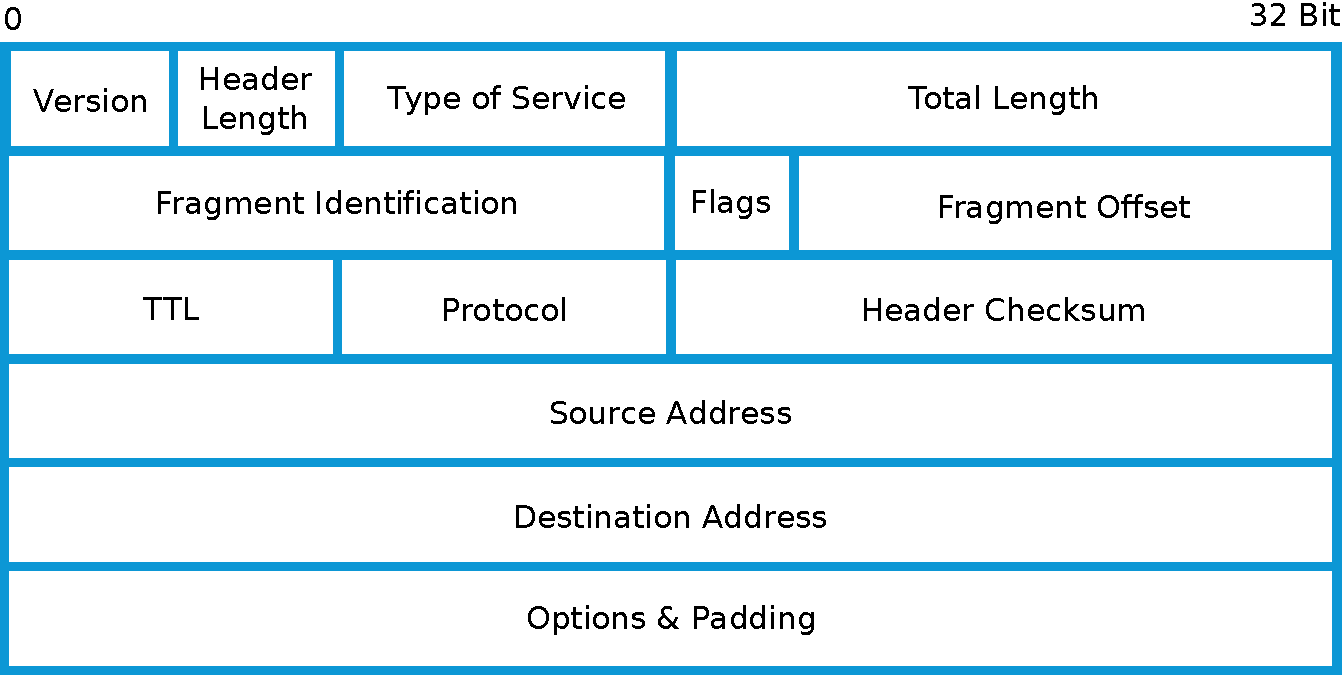
\includegraphics[width=0.87\textwidth]{ipheader.pdf}
    \caption{IP header}
    \label{IPheader} 
\end{figure}

The main conceptual takeaway here is that we are now able to access every field shown in Figure 4.9 of the IP header via the struct ~\cite{35}~\cite{38}. The protocol field, for instance, will tell us whether the upper layer protocol of the packet is UDP or TCP. (If the packet is UDP, our PEP will take no action with it and forward it on. Our PEP only deals with connection oriented protocols). We can calculate the total length of the IP header in bytes, as shown below, by taking the value of the length field and multiplying it by four. The IP header specifies the length of the header in D-WORDS which are 4 bytes in length ~\cite{2}. This knowledge will then allow us to locate the start of any TCP header following the IP header.\\

\begin{lstlisting}
unsigned short iphdrlen;
iphdrlen = ip->ihl*4;
\end{lstlisting}

The main fields we should be aware of are the last two fields, namely source address {\tt (saddr)} and destination address {\tt (daddr)} which are both 4 byte or 32-bit fields in the header and the iphdr struct respectively. The destination IP address {\tt (daddr)} is especially crucial as the {\tt daddr} is needed for the assembly of an ARP request (ARP resolution) which is crucial for acquiring the target destination MAC address that our packet injector will be sending spoofed packets to. The IP header and IP destination address are needed for the end to end connectivity in the network ~\cite{1}. As programmers, we can determine whether we need to manage this packet based on this information. For instance, if the packet is headed to the target network, we need to manage the packet. Otherwise if it is a packet to the local network or alternatively a packet headed specifically to the proxy machine hosting our PEP, we simply forward the packet.  \\

\subsubsection*{TCP header struct:}

Our PEP will deal exclusively with connection orientated protocols, (as do most PEPs generally), so we will focus on Transmission Control Protocol(TCP) rather than UDP. Regarding coding, this means our PEP will read the protocol portion of the IP header in our buffer, and only interact with TCP packets. Non-TCP packets will simply be forwarded without further ado.\\

The TCP header structure as defined in tcp.h can be viewed in Appendix A. It is possible to construct our own TCP struct theoretically, but the TCP header struct already exists in a library which we can easily import. \\

\noindent\textbf{Example of tcphdr struct library import:}\\
{\#}\textcolor{orange}{include}<netinet/tcp.h> \textcolor{red}{{\//*} \emph{Provides declaration for tcp header}{\/*/}} \\

As with the Ethernet header and IP header structs, the concept behind the TCP header struct is precisely the same. The tcphdr fields, as seen in Fig 4.10, will all be accessible via the tcphdr struct (See Appendix A to view the {\tt struct tcphdr} as defined in the tcp.h library). All that is required now is to create a pointer of type {\tt struct tcphdr}. Using our buffer as a starting point, we increment our pointer by the size of the Ethernet header(14 bytes) plus the size of our IP header, so that it points at the start of the TCP header ~\cite{38}.\\

\noindent \textcolor{red}{struct} tcphdr *tcp=(struct tcphdr*)(buffer + iphdrlen + sizeof(struct ethhdr)); \\

Now that we have a pointer to the TCP header in our buffer, we can do the following:\\

\begin{enumerate}
\item We can identify what flags are set which will identify what type of packet we have in our buffer (is it a SYN, ACK, SYN + ACK, FIN, RST?).
\item Being able to identify the type of packet we have will allow us to make decisions about what action we take with the packet. (e.g. do we need to forward it, absorb it, forward it, cache and forward etc.).
\item We can trace the sequence and acknowledgement numbers of the packets. This information will be useful once we begin our proxy functions for our PEP.\\
\end{enumerate}

\begin{figure}[h!]
    \centering
    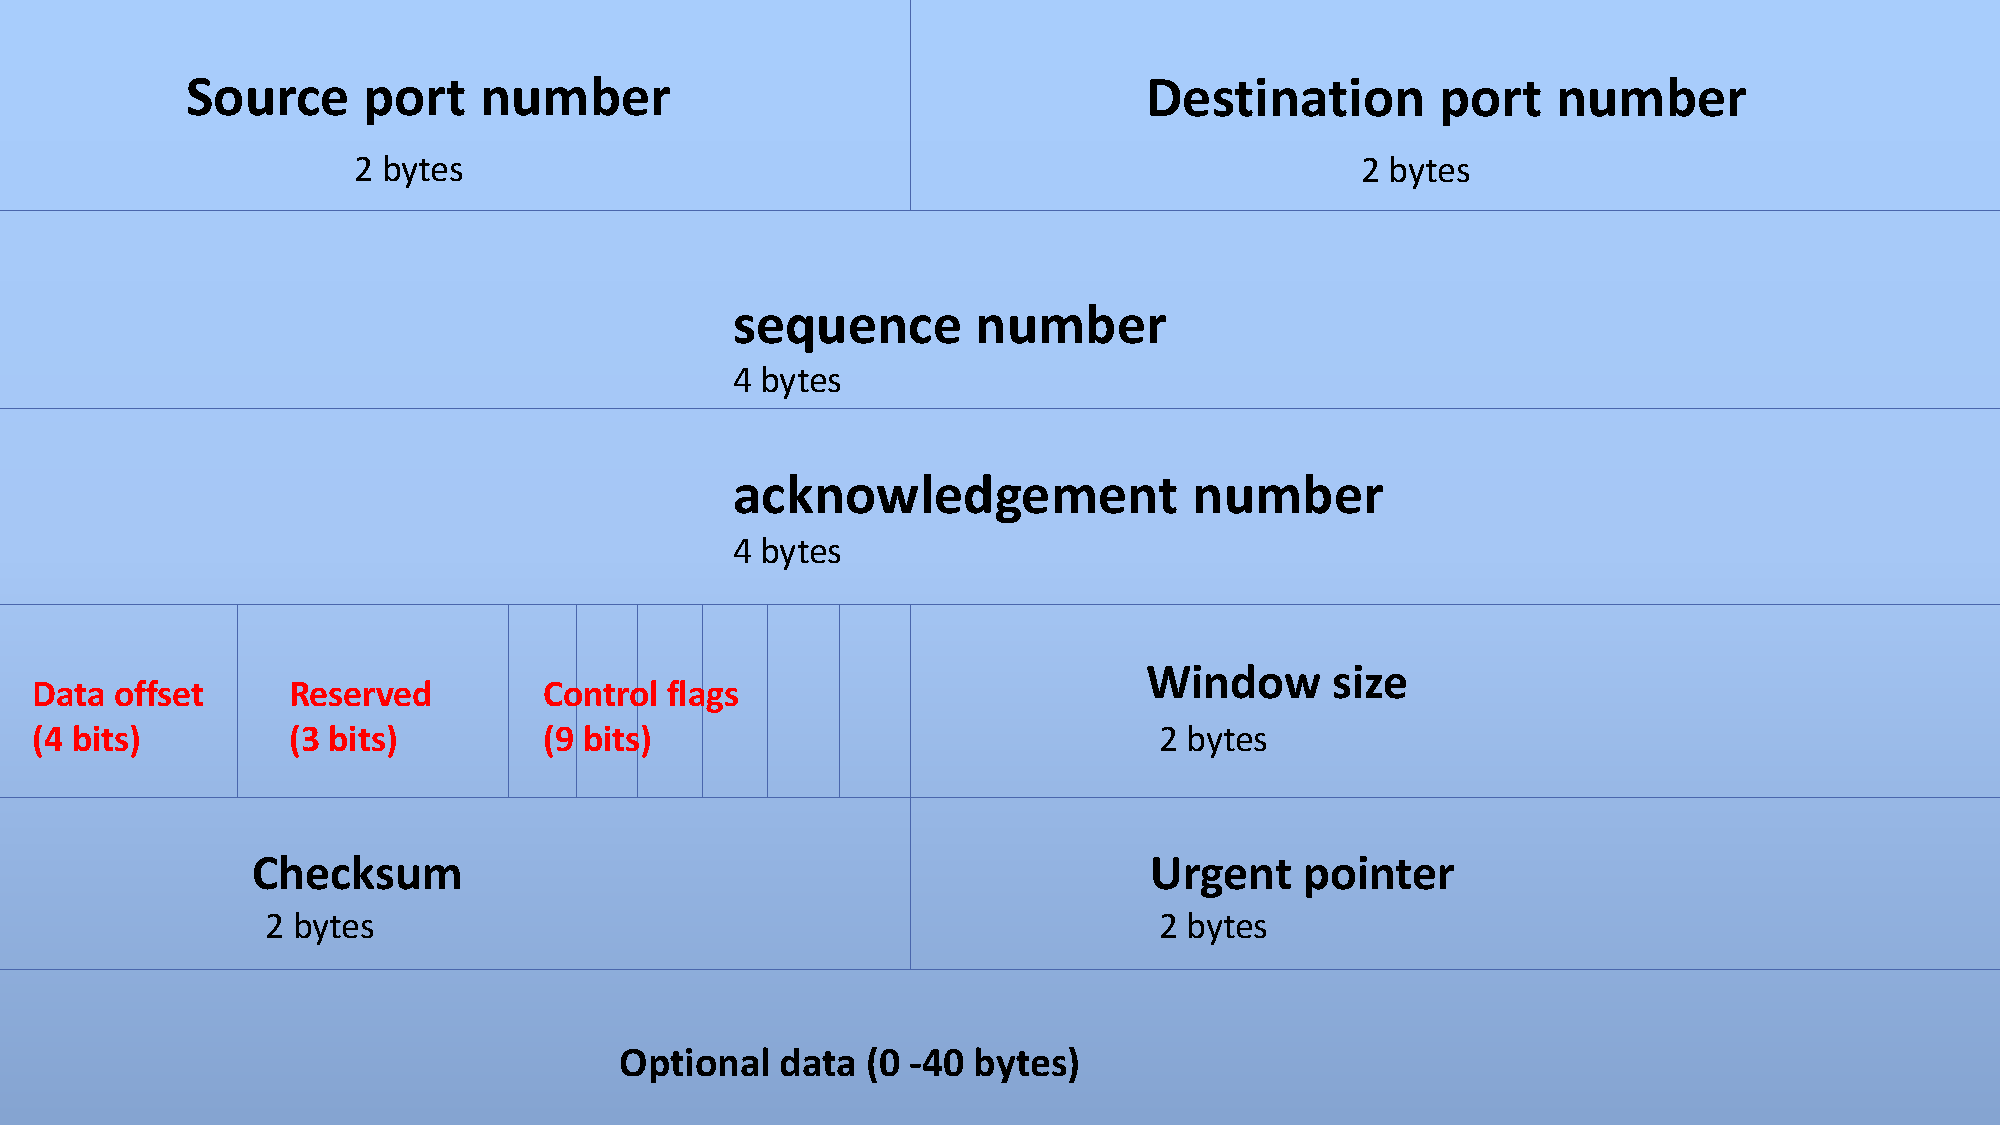
\includegraphics[width=0.95\textwidth]{TCPHeaders.pdf}
    \caption{TCP header fields}
    \label{TCPHeader}     
\end{figure}

These are just a few examples of what can be done. As well as being able to inspect the packets in our buffer, we will also be able to create duplicate packets and alter fields within them to suit our proxy purposes. \\

The control flags are defined in the hexadecimal format each represented by the FIN, SYN, RST, PUSH, ACK and URG flag as number 1, 2, 4, 8, 16,  and 32 respectively. The flags play a key role in our PEP as we will be setting these flags to suit the purposes of our packet injector when we assemble our spoofed packets. When we create an ACK response to a received data packet in our buffer, for instance, we would set the ACK flag to 1 and set all other flags to 0. We would have to create a duplicate of the packet headers but alter the flags so that only the ACK flag is set to indicate this is an ACK response ~\cite{35}. \\

The ACK packet we created would also need to have its sequence number and ACK number set accordingly. The source port number and destination port number fields would also need to be swapped when we create the ACK packet. We would also need to swap the source IP and destination IP addresses in the IP header of the packet. Similarly we must also swap the source and destination MAC addresses in the packets Ethernet header. In all of these cases, this requires the recomputation of the header checksums ~\cite{38}.\\

\subsubsection{Summation of the header structs usefulness for a PEP}
From a conceptual standpoint, the underlying message the reader may wish to take away from these last three sections is that the structs give a programmer the means to do two significant things. Firstly, the structs allow us to read the contents of a packet received on an interface we have bound our raw socket sniffer to. Secondly, the structs allow us to use information from the packets to build our own datagrams and packets for forwarding through our PEP via packet injection. For example, if we receive a raw network packet into our buffer that is a data packet, we can read its source MAC address and source IP address from the Ethernet and IP headers respectively, then replicate them as our destination MAC and destination IP addresses when we construct our ACK packet ~\cite{35}~\cite{38}. We will explore this more in our Proxy chapter. If the received raw packet needs forwarding, we can use the destination IP address to do an ARP lookup in our ARP table cache or to build an ARP-Request Packet. This leads us to our next section on Address Resolution Protocol (ARP) needed for forwarding of packets. \\

\subsection{Finding the MAC address for forwarding packets}
We now have the means to receive raw packets and read the header and data information coming from any particular interface we have bound our raw socket to. We can assemble an ACK reply to send back to the sender based on this information (we can glean their IP and MAC addresses via the sniffer) but forwarding the packet onto its next hop MAC destination requires another step. \\

As Fig. 4.9 shows, the incoming packet will have its source IP address and the destination IP address while the incoming Ethernet header holds its source mac and the destination MAC address (the MAC address of our sniffing interface). Forwarding the message onto the next hop in the Ethernet data link layer requires a destination MAC address, but we only have the destination IP address to help us forward the packet ~\cite{1}~\cite{2}.\\

Usually, the kernel would take care of finding the next hop MAC address for our packet using its own internal ARP table, forwarding the packet out the interface we specified in our C code onto the next hop MAC. This was not the case, however, and the kernel was overriding that command and sending it out the interface it deemed best. Often, the combination of being sent out the wrong interface and the MAC address of the next hop based on that interface, caused many unforeseen problems with our PEP. For starters, it meant that we could not control where the outgoing packets from our PEP would go and that defeats the purpose of having a PEP in the first place. It became clear at this point that we must code for the Ethernet layer and manually set our destination MAC address as well. We needed to create our own Address Resolution Protocol (ARP) request frames and ARP table cache to store these MAC addresses. \\

Address Resolution Protocol (ARP) is the mapping of a layer 3 network address to a layer 2 link layer address in the OSI model. In other words, ARP is used to map an IP address to a MAC address and (vice versa as well) ~\cite{1}. Given we can glean the destination IP address from the sniffed raw packet, acquiring the destination MAC address is achievable in two ways. We can use the destination IP address to look up the MAC in the ARP table. If there is no IP to MAC mapping entry found in the table, then we can retrieve the MAC address via an ARP request and listen for an ARP reply. 

\subsubsection{Brief summary of address resolution protocol (ARP)}
When a host is performing an ARP, the destination IP address the host wants to communicate with is known, but the destination MAC address is unknown. The host will broadcast an ARP request packet that will be received by all other hosts in its local network. \\

\begin{figure}[h!]
    \centering
    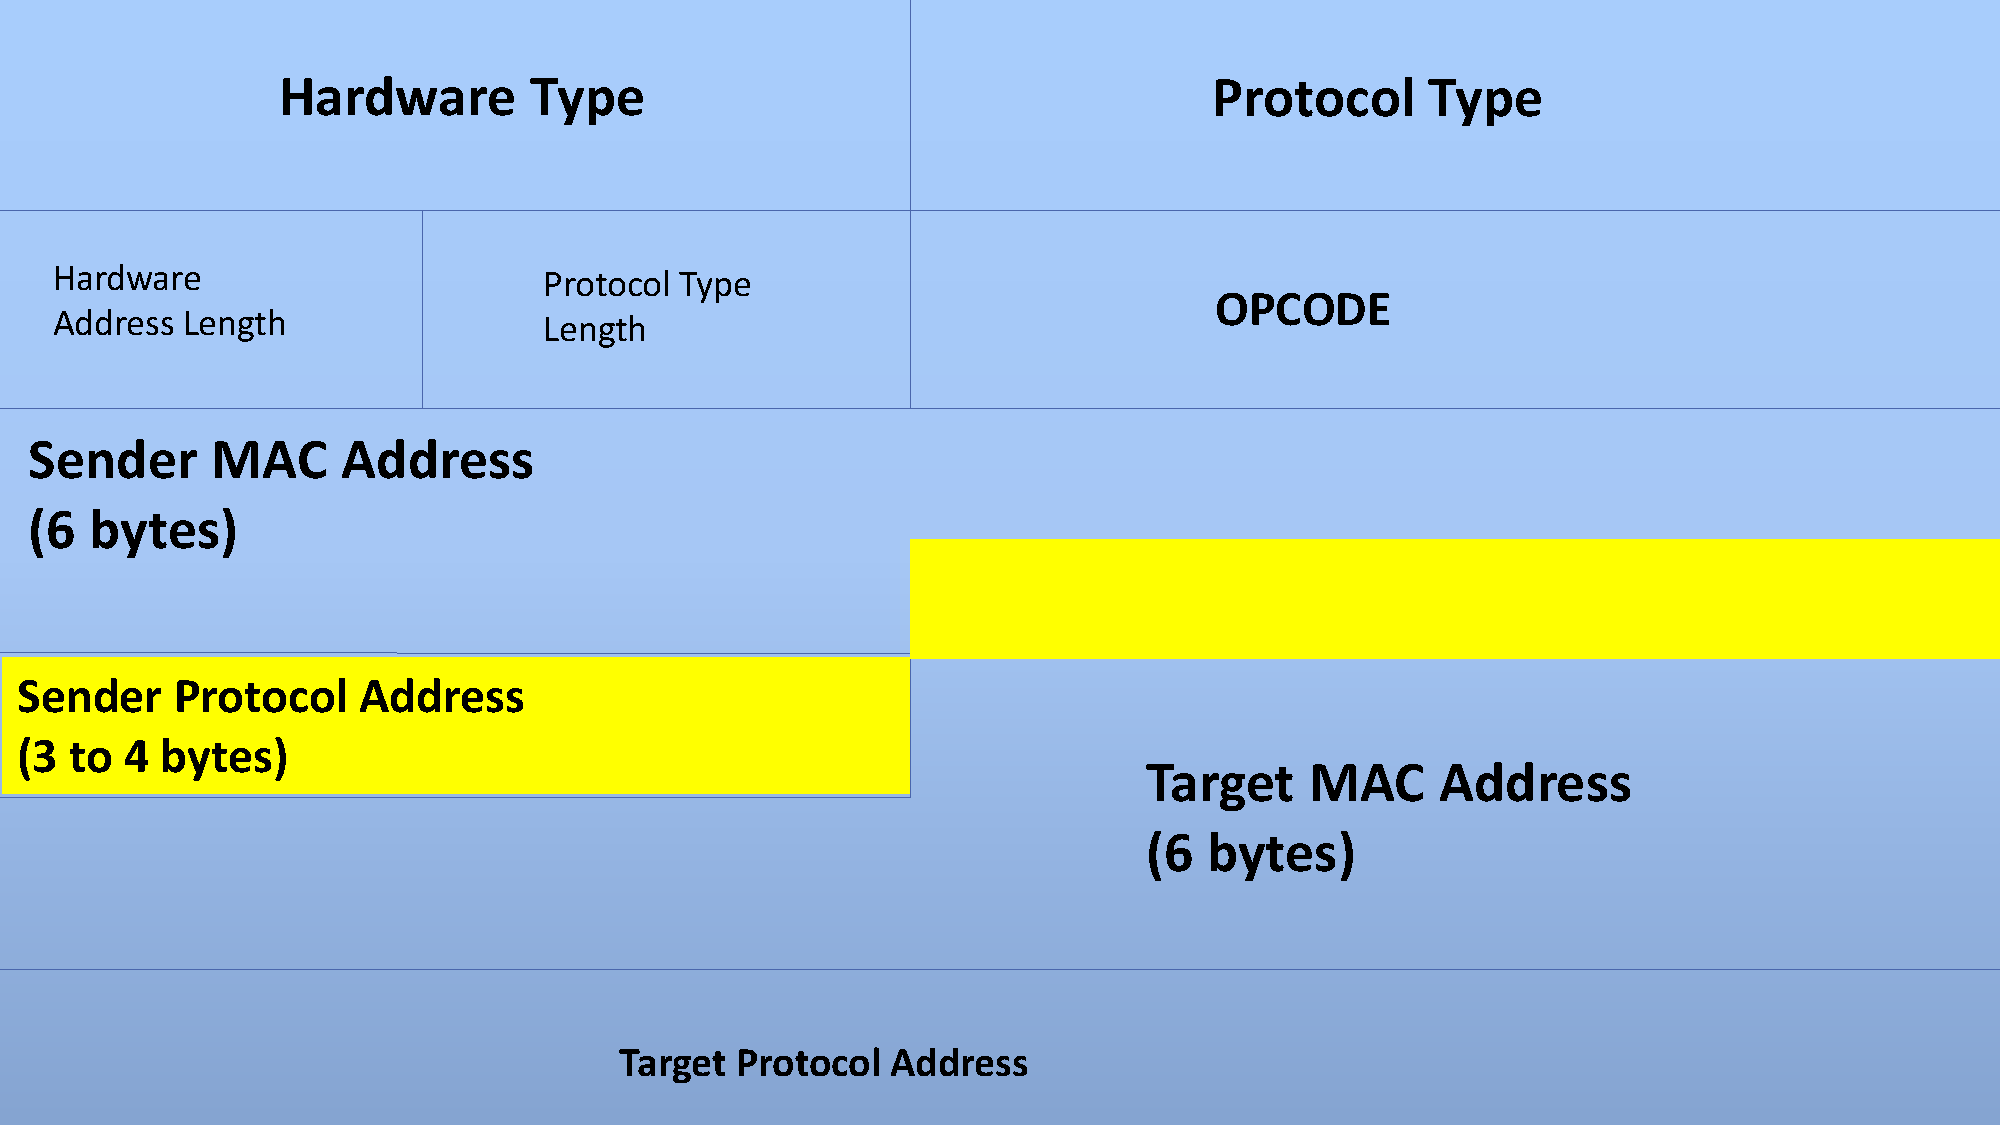
\includegraphics[width=0.95\textwidth]{ArpHeaders.pdf}
    \caption{ARP Header fields}
    \label{ARPHeader}
\end{figure}

It does this by setting the target hardware MAC address field as shown in Fig:4.11 ARP header to all zeroes 00 : 00 : 00 : 00 : 00 : 00. The destination MAC address in the Ethernet header is then set to FF : FF : FF : FF. This is a unique MAC address that ensures the ARP packet is broadcast to every host computer in the local network subnet~\cite{1}~\cite{2}. The concept behind the broadcasting of an ARP request is straightforward. The ARP request is asking each host in the broadcast domain the question "who has this IP address? (destination IP address)". The host computer with this IP address will respond "I have this IP address" and resend confirmation of this with an ARP-Reply packet that is almost identical to the ARP request in structure. The significant difference is that the ARP-Reply will be sent back with the target hosts MAC address as its Sender Hardware Address field ~\cite{1}~\cite{2}. \\

This  Sender Hardware Address is the Destination MAC address information the sender required from the host. The sender can now fill in its packets "Destination MAC address" field in its Ethernet header with the ARP-Reply  Sender Hardware unicast MAC address (singular) rather than the initial broadcast address (FF : FF : FF : FF : FF : FF). The packet is then forwarded to the host on that destination MAC address subnetwork ~\cite{1}. \\

When the destination IP belongs to a network beyond the local network to whom the interface of the current host is connected to  (not an IP on PEPs interfaces subnetwork or local network), the ARP request will retrieve the MAC address of the router interface that is the default gateway to the destination network. The protocols of the routers and switches in the outer network will take care of delivery of the packet from then onwards ~\cite{1}.

If the destination IP belongs to a host in the local network, then the MAC address of that host will be returned to the sender of the ARP request. The next step is to create our own ARP table to track the MAC to IP address mappings. It would not be efficient programming to send an ARP request every time we need to forward a packet. Therefore we need an ARP table which can cache these IP to MAC mappings. The general idea is that our code will check the ARP table first to see if we already have a MAC address mapping for an IP address before sending any ARP-Request packet ~\cite{1}~\cite{2}. (i.e. We initially start with an empty ARP table and we progressively populate the table with the responses to ARP requests that we send. There is also a timeout for each ARP entry).

\subsubsection*{ARP table:}
Each host machine on the subnetwork has an ARP look-up table that keeps a record of the IP address mappings to MAC addresses it finds ~\cite{1}~\cite{41}. Before making an ARP request, the host sender checks its own ARP look-up table to see if it has already ARPed this IP address and thus has the MAC address cached in the table. If so, an ARP request is not required. If there is no existing entry, an ARP request is sent, and upon return of the ARP reply, a new IP address to MAC address record is cached in the ARP table ~\cite{1}~\cite{2}~\cite{41}.\\

\subsubsection*{What We Need To Do:}
This means we need to create an ARP request packet ourselves to wrest control from the kernel. In our case, this also involves creating an ARP struct that will store the ARP reply information when the request is answered and our own ARP look-up table to cache IP address mappings to MAC addresses. As the ARP Header is not readily found in a library for import, we will have to create our own ARP Header struct which is very easily done: \\

Firstly, in dealing with the construction of a basic ARP look-up table, it must be built to allow us to store MAC addresses with their corresponding IP addresses as keys while also having a fast and CPU efficient method of searching for these MAC addresses based on their IP address key ~\cite{1}~\cite{41}. We settled on a binary search tree model for the table that would be able to perform  this function. The first step is creating another struct aptly named "node" ~\cite{42}. \\

\begin{lstlisting}
struct node {
	uint32_t ip;
	uint64_t mac;
	struct node *left, *right;       
}
\end{lstlisting} 

For this thesis, we assume here that the reader is familiar with binary search trees (see Appendix B) ~\cite{42}. There is a function in our code that takes the IP address and our BST node struct ARP table to look up a MAC address in the ARP table. Our code also has an insert function that inserts new nodes to the ARP table. To create our BST search tree ARP table, we simply declare a pointer of type {\tt struct node* arpTable} which we will assign memory to via {\tt malloc()} in a later part of our code ~\cite{39}.

\subsubsection*{ARP header struct}
As in the previous section, our ARP Header struct will contain attributes corresponding to the fields in an actual ARP Header. We are using C language, so we simply declare a variable of:\\

\begin{itemize}
\item \textbf{typedef struct} arpHeader arphdr\\
\end{itemize}

Next we declare our struct that will take on the fields of an actual ARP header:

\begin{lstlisting}
struct arpHeader {
    uint16_t htype;
    uint16_t ptype;
    uint8_t  hlen;
    uint8_t  plen;
    uint16_t opcode;
    uint8_t  sender_mac[6];
    uint8_t  sender_ip[4];
    uint8_t  target_mac[6];
    uint8_t  target_ip[4];
};
\end{lstlisting}

Our C code for our PEP implementation will fill this struct with the information we receive from the sniffer. See Fig 4.12 to see how this is actioned in our C code. \\

\begin{figure}[h!]
    \centering
    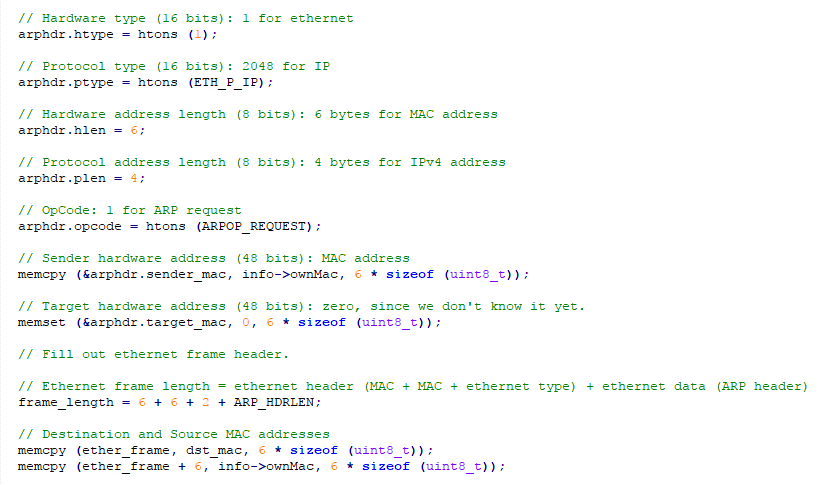
\includegraphics[width=0.9\textwidth]{Capture.PNG}
    \caption{ARP Header}
    \label{fig:Filling fields of ArpHeader struct}
\end{figure}

To summarise, when we receive a packet that needs to be forwarded, we check our ARP table to determine whether we already have a MAC address cached for the destination of the packet IP address. If not, we create an ARP-Request to find the MAC address. Once we have constructed our ARP header, we can send out an ARP request to our local network or the gateway interface.\\

With the destination MAC address returned, we are at a stage where we can now forward the IP/TCP packets we have received on the sniffing interface to their destinations. This leads into the next section which deals with our proposed solution and our methodology for building our proxy logic. \\

\subsubsection{Forwarding the complete packet with the sendto() function}
Once we have a packet assembled and complete with forwarding MAC address, the final step is to forward the packet. Socket programming has a {\tt sendto()} function that completes this process ~\cite{35}~\cite{38}. \\

\noindent{\tt \textbf{bytesSent} =  \textcolor{blue}{sendto}(interface->txSocket, packet->packet, packet->packetSize, 0, (\textcolor{purple}{struct} sockaddr *) \&interface->device, \textcolor{blue}{sizeof} (\textcolor{purple}{struct} sockaddr\textunderscore ll))};\\

The code excerpt above is from the code we use for our PEP. The code makes use of a customised struct created for the incoming and outgoing interfaces of our PEP which will be explained fully in the implementation section of our PEP. The above code also makes use of a struct sockaddr\textunderscore ll (see Appendix B) which allows us to access the link layer for assembly of the Ethernet header. The {\tt sendto()} function takes in six parameters as follows:\\

\begin{itemize}
\item The first parameter is the raw socket we are using for sending: {\tt \textcolor{blue}{int} \emph{sockfd}}.
\item The second parameter is the buffer holding the packet/data for sending: {\tt  \textcolor{blue}{const void} \emph{*buf}}.
\item The third parameter is the length of the buffer: {\tt  \textcolor{blue}{size\textunderscore t} \emph{len}}
\item The fourth parameter are flags which we do not use in our code {\tt  \textcolor{blue}{int} \emph{flags}}.
\item The fifth parameter is the {\tt struct sockaddr} cast pointer to a {\tt struct sockaddr\textunderscore ll} named \emph{device} (see Appendix B) which is a field in the abovementioned customised struct for the incoming and outgoing interfaces of our PEP. The {\tt struct sockaddr\textunderscore ll} contains the forwarding MAC address for the packet/data that is being sent: {\tt  \textcolor{blue}{const struct} sockaddr \emph{*dest\textunderscore addr}}.
\item The last parameter is the size of the struct sockaddr\textunderscore ll in bytes: {\tt  \textcolor{blue}{socklen\textunderscore t} \emph{addrlen}}.\\
\end{itemize}

If the packet is sent successfully, the call returns the number of bytes sent. On error, -1 is returned. This completes the forwarding packets section. The next section covers our proposed solution and the PEP logic and implementation in detail ~\cite{35}~\cite{38}.

\section{Our proposed solution}

As mentioned earlier in the PEP history section, most PEP implementations which deal with satellite link latency adopt the TCP-splitting/connection breaking architecture ~\cite{6}~\cite{14}. Recall that a connection-breaking PEP terminates the connection from one end and opens a connection to the other, such that there are two different connections with different packets, sequence numbers, congestion windows and advertised windows, etc., between the PEP and the two respective endpoints. In a connection-breaking PEP, only the TCP payload data in the packets moves from one connection to the next ~\cite{6}~\cite{14}. The solution offered in this thesis is a non-connection breaking PEP because:\\

\begin{itemize}
\item The PEP does not de-encapsulate TCP packets such that only the payload gets forwarded. The same data packets are seen either side of the PEP, except that retransmissions of packets are only seen on the side of the PEP on which they were lost.
\item The sequence numbers on forwarded packets remain the same. 
\item Only the original TCP sender maintains a congestion window, at least at this point. Future modifications to our PEP may also maintain this window.\\
\end{itemize}

It will, however, interfere with the connection by: \\

\begin{itemize}
\item inserting ACKs when there are none from the receiver yet.
\item intercepting ACKs when an ACK has already been sent to the sender by the PEP.
\item rewriting the TCP checksum and in future/modified versions of this PEP, possibly the advertised window to the sender.\\
\end{itemize}

Our PEP solution aims to partially mitigate some of the problems caused by breaking the end to end rule of the Internet. The next section will elaborate on what these problems are, and then this thesis will outline the proxy functions of our PEP. 

\subsection{Non-Connection breaking PEP}
The novelty of our solution is that it does not break the end to end architecture of the Internet which in turn breaks end to end reliability at the transport layer ~\cite{6}~\cite{13}~\cite{14}. \\

Breaking the fundamental end to end principle of the Internet can create issues in itself. Connection breaking PEPs will not be able to deal with IPsec connection flows or Virtual Private Networks. Encrypted packets under an IPsec flow, for example, will encrypt the IP Payload which includes the TCP header. Connection breaking PEPs need to be able to read the TCP header of the packet in order to send ACKs back to senders and to perform the optimisation procedures effectively. IPsec prevents the reading of TCP headers and therefore hampers these connection breaking PEPs ~\cite{14}.\\ 

Another issue that may arise from the breaking of the end to end TCP semantics is the "Where's the money" problem that results from the consequent breakage of TCP end to end reliability ~\cite{13}. This is one \textbf{real world} negative consequence of violating the end to end TCP semantics of the Internet whereby we have an intermediate agent sending ACKs back to a sender rather than the actual final receiver. Imagine a scenario where one is doing an Internet transfer of money over a connection breaking PEP link satellite connection. \\

TCP client sends the transfer over the line and the intermediate agent PEP, acting as a proxy server, sends an acknowledgement back to the client confirming the transmission of said funds before creating and forwarding the transfer information to the final receiver. These actions break the fundamental end to end connectivity principle of the Internet but will cause no issues so long as there are no problems in the connection. \\

Problems can arise, however, if there is some break in the connection between the PEP and the final receiver before getting the actual information to the final receiver end. In this case, we are left with an undesirable situation where the sender has received an ACK from our intermediate agent PEP but the data forwarded on by the PEP is lost before it reaches the final receiver ~\cite{13}~\cite{14}. Thus the client believes it has transferred the money successfully when the request for transfer of money to the Internet banking site has actually been lost. This thesis puts forth a non-connection breaking PEP that is an alternative to current end to end breaking PEPs. \\

Unfortunately, our non-connection breaking PEP also does not completely solve this problem yet. The PEP preserves port numbers and sequence numbers and is therefore compatible with protocols that include references to these in TCP payloads (VPNs in particular). The PEP also addresses the breaking of the IPsec flows as our proxy would simply forward these packets without ACKing them to the sender. Our PEP, however, does not optimise IPsec flow performance over the link either. The next section will walk the reader through the proxy logic for our PEP in this thesis.

\subsection{PEP proxying roadmap}
Thus far, this thesis has covered the concept of sockets, raw sockets to create a sniffer and the various data structures used to store packet information gleaned from a sniffing (i.e., bound to our raw socket) interface. The forwarding and assembling of packets via these structs have also been covered. This section of the thesis moves now into the most important phase of our PEP construction: The proxy logic.\\

In other words, this part of the thesis takes the reader through the actions and decisions our PEP will make as datagrams/packets traverse through the PEP. The next section will give more detail on the actual implementation of the PEP, as well as outline the PEP logic that we managed to implement (some aspects of PEP logic had to be left to future work due to time constraints). The results chapter will document the performance of our PEP on our lab's Pacific Islands satellite network simulator.\\

Our PEP will be dealing with multiple TCP connections at any one time. To keep track of these connections, our PEP will need a connection table similar to the ARP table used to keep track of IP to MAC mappings. For this purpose, we will once again use a binary search tree structure. Each node will represent a TCP connection, and within each node, we have a FIFO (first in first out) linked list data structure to represent the data packets from each TCP connection that we cache ~\cite{43}. More detail on the implementation of these structures for our connection table will be given in the next section. \\

This thesis assumes that data structures such as FIFO queues implemented as linked lists ~\cite{43}, are known to the reader. The PEP logic works as follows: \\

\noindent \textbf{Filtering the packets; choosing which packets to proxy} \\
Suppose we have now set up the PEP and it is active and ready for operation. The first action our PEP takes upon receiving an incoming packet is to decide whether it is a packet we need to handle. Our PEP code has a function called {\tt checkRXInterface()} which executes this vetting action of us. This {\tt checkRXInterface()} function will look at all the packets being received on the PEPs incoming interface and simply filter out the packets the PEP should ignore, and enqueue the rest of the packets on the interface's receive queue ({\tt rxQueue}) for processing. \\ 

\emph{For our PEPs incoming and outgoing interfaces, we created a struct called {\tt proxyInterface} that has a receive queue for processing incoming packets and a transmit queue ({\tt txtQueue}) for processing transmission of packets.  More detail will be given in the proxy logic implementation section.} \\
 \begin{figure}[h!]
    \centering
    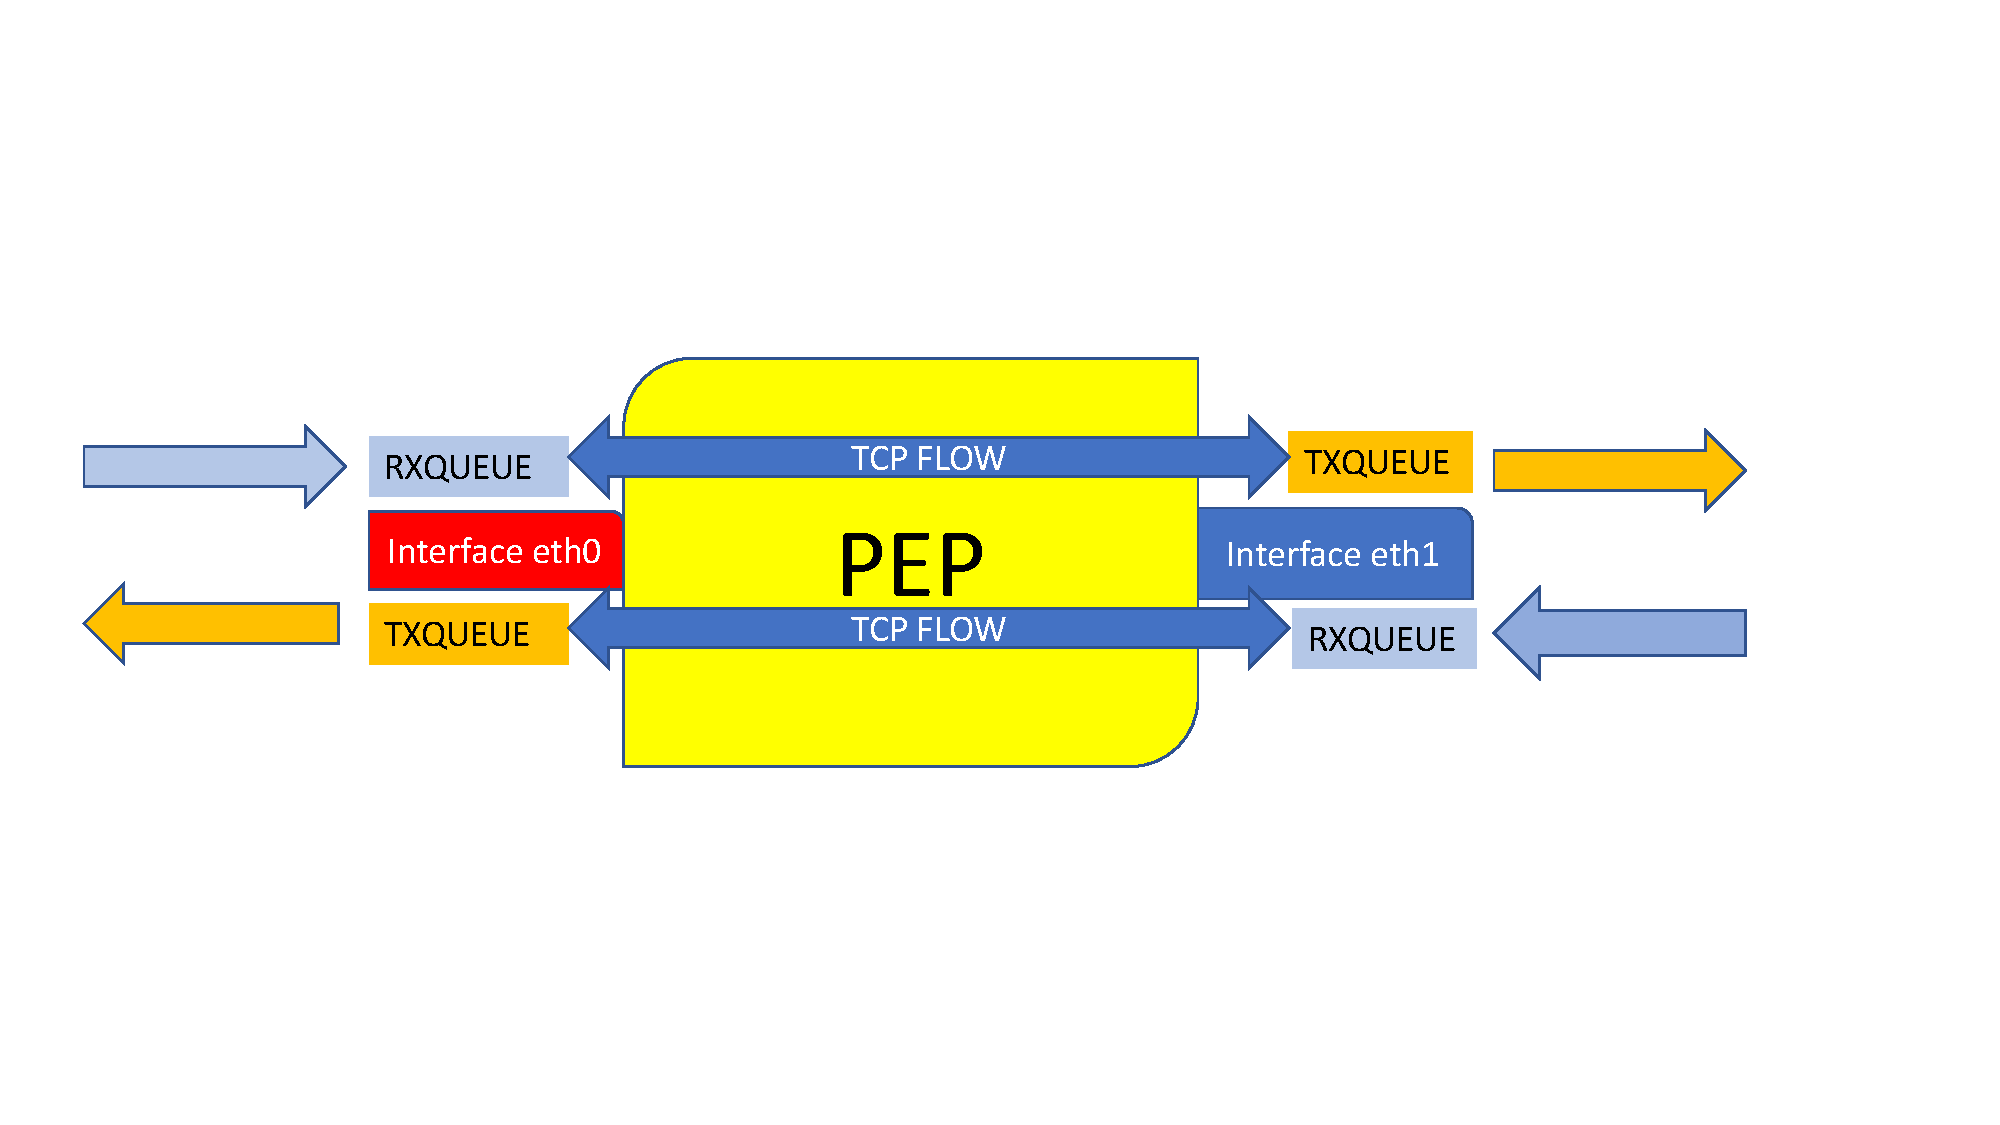
\includegraphics[width=1.0\textwidth]{PEPInterfaces.pdf}
    \caption{The rxInterface and txInterface FIFO queues for both the islandside (eth0) and worldside (eth1) interfaces of the PEP. Note that rxQueues => queueing incoming TCP flows and txQueues => queueing outgoung TCP flows on our PEPs proxyInterface struct.\\}
    \label{PEPInterfaces}
\end{figure}

\noindent \textbf{List of incoming packets our PEP will disregard:}\\
 
There are only three types of incoming packets our PEP will ignore:\\
\begin{itemize}
\item The packets that our own PEP has transmitted and detected on the PEPs  own interface.
\item The packet is directed to the proxy host (i.e., someone is sending data to the computer that our PEP is running on). Our PEP does not need to deal with these packets. There will be other processes on the host computer that can deal with this data.
\item It is a packet directed to another host on the local network of the PEP interface. This host sits on the same side of the PEP as the PEP interface that the packet came in from. \\
\end{itemize}

\noindent \textbf{List of packets our PEP will interact with:} \\

There are only two types of incoming packets our PEP will handle:\\
\begin{itemize}
\item Packets that need to be proxied (i.e., packets that are heading to a network on the other side of our PEP).
\item ARP response packets for an ARP request sent from our PEP. \\
\end{itemize}

The packets listed above are the only ones we are concerned about and that our PEP is designed to proxy (Non-TCP packets will be forwarded on, the PEP will ignore all other packets). The PEP will then enqueue these packets, from the list above, on an interface receive queue (rxQueue) where they will identify the packet as per the list below and apply the appropriate proxy logic accordingly:\\

\noindent \textbf{Applying the proxy logic:} \\

\noindent A) When the PEP identifies an incoming TCP data packet, it must:\\ 

\begin{enumerate} 
\item Identify the TCP connection it belongs to by checking our connection table. If no entry for this packet exists, the PEP creates a new entry for it in our connection table. \\
\item Acknowledge the packet to the original sender (which may have been a PEP on the far side of the sat link, or the original sender). The ACK will eventually need to reflect (in its advertised window field) an idea of how "full" the link currently is. The PEP will know this because it can be configured with the link's queue capacity and because it knows how much data it has sent to the link recently (future work). \\
\item Forward the packet to the final recipient (which theoretically may sit behind another PEP). \\
\item Cache the packet (unless it is already in the cache, i.e., we have received retransmission in which case we resend an ACK to sender) in the FIFO queue of the corresponding TCP connection node in our connection table. (We want to keep a copy of the packet in case we need to retransmit it. If we do not receive an ACK back from the final receiver within a certain allotted time, we assume the packet has been lost/dropped and must retransmit).\\
\end{enumerate}

\noindent B) When the PEP identifies an incoming packet that belongs to a TCP IPsec connection or VPN connection:\\

\begin{enumerate}
\item Do not proxy. Treat as an unknown protocol.
\item Forward all packets from this connection flow onto next hop without alteration. (Note, all non-TCP protocol packets are also forwarded in the same way).\\
\end{enumerate}

\noindent C) When the PEP sees an incoming ACK for a data packet it has cached (i.e., already ACKed to the original sender), it must:\\

\begin{enumerate}
\item Identify the TCP connection the ACK belongs to by checking our connection table. 
\item Delete data packets that the ACK relates to from the cache. This includes any packets whose TCP sequence number + TCP payload length is \emph{below} the ACK number in the ACK packet. Do not forward the ACK packet.
\item Dynamically recalculate the RTT. This calculation is based on the time we receive an ACK, minus the time of sending for the packet with the highest sequence number covered by this ACK. (When our proxy sends a packet, it is also cached simultaneously. Thus we can find the precise time we send a packet via its time of insertion into our cache).
\item Relays the time of the \emph{updated RTT} x 1.3 to another function (housekeeping function which will be detailed later) which periodically traverses the cache and uses this time period to schedule retransmission of unACKed packets. Simply put, the function determines which packets have been in the cache for a time of \emph{RTT x 1.3} or longer, and retransmits them.

\item If the ACK does not cover any data packets in the cache, forward the ACK. It is probably either a duplicate ACK or part of a FIN + ACK, for example, and needs to be forwarded on.\\
\end{enumerate}

\noindent D) When the PEP sees an incoming FIN or FIN+ACK packet for a connection, it must:\\

\begin{enumerate}
\item Forward the FIN or FIN+ACK to the recipient.
\item Set an expiry time on any data packet entries in the outgoing interfaces cache for this connection.
\item Remove the connection from our connection table after the previously mentioned expiry time has elapsed. \\
\end{enumerate}

\noindent E) When the PEP sees an incoming RST packet for a connection, it must:\\

\begin{enumerate}
\item Forward the RST to the recipient.
\item Delete any data packet entries in the cache for this connection on incoming and outgoing interfaces.
\item Remove the connection from our connection table. \\
\end{enumerate}

\noindent F) When the PEP sees an incoming ARP packet, it must:\\

\begin{enumerate}
\item Check if it is an ARP request or ARP response. If it is an ARP request, PEP takes no action. Kernel will handle the request.
\item It is an ARP response. Check if the sender IP address contained within the ARP response is already in the ARP table. If not, add new sender IP to MAC entry in the table.
\item Enqueue any packets that were waiting for the MAC address to arrive. \\
\end{enumerate}


\noindent \textbf{Housekeeping for the PEP:}\\
In addition to the reactive PEP logic described above, it is also imperative to maintain regular housekeeping for the PEP [6]. The housekeeping aspect of the PEP periodically performs a set of actions that clean up our PEP packet caches and keep them up to date. These actions include:  \\ 

\begin{enumerate}
\item Regularly traversing the data packet caches of all active TCP connections utilising our PEP. As the housekeeping function traverses the data packet caches, it will retransmit all cached packets within a TCP connection node, which have not been ACKed within 1.3 x the expected round trip time (RTT). \\
\end{enumerate}

\noindent The housekeeping function should also take care of cached packets that belong to terminated connections and also act accordingly for cases where a receiver has become unavailable. Perhaps the receiver has malfunctioned, or there is some network issue preventing it from receiving packets. Whatever the reason, this scenario must be taken into account:  \\ 

\begin{enumerate}
\item If the housekeeping function comes across cached packets whose expiry time (after a FIN or FIN+ACK) has passed, the function will not retransmit these packets. The expired time signals that the TCP connection has terminated by this stage, so any cached packets belonging to the terminated connection need clearing instead.\\
\item It is necessary to set a cap on the number of retransmissions permitted for any packet (which could be made configurable eventually. We currently hardcode this number.). If a maximum number of transmissions is not set, we could get undesirable effects such as the receiver being unreachable for some reason, but our PEP is continuously trying to retransmit the packet ~\cite{6}. To prevent this, we will set a cap such that if the number of retries reach the cap, we stop retransmitting the packet. In a future modification of the PEP, we may send a RST packet to both end hosts.\\
\end{enumerate}

When we first activate our PEP, we must initially configure an RTT timeout value based on an estimate. Bear in mind that this PEP is being designed with the Pacific Island satellite Internet connection scenario in mind ~\cite{3}~\cite{4}. Our PEP will be tested on the University of Auckland's satellite testbed which simulates the satellite connectivity for the Pacific region covering Niue, Tokelau and Rarotonga [21]. Therefore we can base this first RTT timeout estimate on the Pacific island satellite infrastructure. The most commonly used type of satellite link in this region is through geostationary satellites.\\

For example, when the PEP sits on the world side of a GEO sat link to an island, data packets that made it to the island receiver should be acknowledged no later than the satellite RTT (~500 ms) plus whatever the maximum queue sojourn time at the satellite input is (depends on link rate and queue capacity), plus any small delays on router queues and for processing on the island ~\cite{4}. The latter two components will be small - just a few ms (say less than 10). So if we have a 16 Mbps link (2 MBps) with a 1MB queue, the queue sojourn time is ~500 ms, and all ACKs should have arrived after at most 1010 ms. Once the first ACK is received, our ACK function will dynamically calculate a new RTT and subsequent new cache packet timeout for retransmission from this time forth.\\

\subsubsection{PEP flowchart for PEP logic}
This PEP flowchart features one more important element in our overall PEP logic that has not been mentioned as of yet. Thus far, this section has discussed a TCP connection table (binary search tree structure) for keeping track of TCP connections and the caching of packets in FIFO queues (linked list structures) within the TCP connection nodes ~\cite{42}~\cite{43}. We also modified our ARP table nodes to include the FIFO queue field for storing of packets awaiting MAC address from ARP responses for a particular IP address. To recap, the reason these packets are being cached in these FIFO queues is that: \\
\begin{enumerate}

\item The packet has been forwarded, but we are keeping a copy of the packet in cache until we receive an ACK back from the final recipient. If we receive an ACK within the estimated RTT, we remove all cached packets covered by the ACK. If not, we assume the packet has been dropped. The packet will then be retransmitted via the housekeeping function. \\
\item The packets are awaiting a next hop MAC address via an ARP response before they can be forwarded. The ARP table has been checked, and no entry was found, so an ARP Request was sent. If a response is not received within an allotted timeframe, another ARP Request must be sent. \\

\end{enumerate}

\begin{lstlisting}[language=C]
struct {
    uint32_t ip;
    uint64_t mac;
    node *left, *right;
    time_t insertTime;
    packetQueue * packets;
};
\end{lstlisting}

\noindent \textcolor{blue}{The struct node for the ARP table contains a FIFO linked list queue. The \textbf{\textcolor{red}{{\tt packetQueue* packets}}} is a waiting queue for packets that do not have a MAC for forwarding yet}\\


If we have a packet that needs forwarding and we do not have a MAC address for it yet, the packet is placed in the ARP table entry node queue above and will then be enqueued to the interface transmission queue from there once a MAC arrives from an ARP response. In all other cases, the packets are put straight into the interface transmission queue when we have an existing MAC. In future cases, to avoid complication, we will just assume that this is what the PEP does if we do not have a MAC address. Thus for subsequent sections, the thesis will only discuss queueing packets at the transmission interface, but for simplicity, the reader can remember or keep in mind that this means we may have to queue them at the ARP table entry first.\\


At some point, all of these FIFO queued packets need to be handled, sorted and processed accordingly. The missing element that ties all of these processes together and completes our PEP logic is a struct we created for the sniffing interface:\\
\begin{lstlisting}
struct proxyInterface {
    const char * name;
    uint32_t ip;
    uint64_t mac;
    uint32_t netmask;
    uint32_t network;
    uint32_t gateway;
    int rxSocket;
    int txSocket;
    struct sockaddr_ll device;
    struct packetQueue* rxQueue;
    struct packetQueue* txQueue;
    struct node * arpTable;
    struct connectionCacheNode * cache;
    int cacheConnections;
    int cachePackets;
    int arpEntries;
    int arpPackets;
    int retries;
};
\end{lstlisting}

Note that the struct proxyInterface contains two other structs that we have discussed in the previous chapter. We have the connectionCacheNode* cache which is for the binary search tree TCP connection table ~\cite{42}. (Each node in the binary tree represents a separate TCP connection) ~\cite{42}. The struct proxyInterface also has the previously discussed struct node* arpTable for IP to MAC mappings.\\

With the help of the ifreq struct discussed earlier, we will be able to transfer all the necessary fields for the interface we have bound our PEP to. (e.g. interface IP, mac, netmask, network, gateway IP). The main two new features of our customised struct, however, that this section would particularly want to draw the reader's attention to, are the struct packetQueue* rxQueue and struct packetQueue* txQueue because they both relate directly to our PEP logic flowchart. (Also worth a mention is the struct node* arpTable as we have added a struct packetQueue* field within that node struct to store packets that are awaiting a forwarding MAC address from an ARP response).\\

The struct packetQueue is as its name implies it to be: a queue for packets. The reader may recall that this is the same customised linked list struct we have used to create our FIFO queues in our binary tree connection-table cache nodes (See Appendix B).\todo{promise} In this instance, we use these queues for the packet flow on the interface.\\

The rxQueue (receive queue) represents the queue of packets coming into the interface. Most of the PEP logic is associated with this queue as our PEP makes all of its decisions based on the type of packets that are being dequeued off the rxQueue. (See PEP logic in Proxy RoadMap section). For example, if we receive a packet that has no MAC mapping in the arpTable, we resend an ARP request and queue it in the arpTables packetQueue struct where it will remain until it receives an ARP response.\\

The txQueue (transmission queue) is much simpler as it represents the packets ready to be sent out from the interface. For example, this would include the arpTable packet that has just received an ARP response packet. Our code logic will enqueue the packet on the interface txQueue ready for transmission. \todo{add these structs to Appendix} \\

The programming of the PEP  ensures it traverses and processes the rxQueues and txQueues in a continuous loop. In the main function (of our code), we have these process functions set up in a perpetual \emph{while loop} so that we are continually enqueuing packets coming into our interface on the rxQueue and packets forwarded from our interface in the txQueue. The housekeeping function is also repeatedly called in this perpetual loop but an \emph{if statement} surrounds the function with a timer condition to make sure it is only executed at timely intervals (more detail on the timing mechanism will be given when discussing the implementation of the housekeeping function later in the thesis).\\

The flowchart/use case diagram provides a visualisation of the PEP logic and how it interacts with the interface queues. \todo{make flowchart and place here}It may be useful for the reader to refer to this chart when reading through the PEP logic section and it may also be useful for the next section "Implementing The Proxy Logic In Our PEP" which will frequently refer to the PEP logic often. 

\subsection{Implementing the proxy logic in our PEP}
In the previous section, this thesis presented a high-level overview which gives a walk-through of the PEP logic detailing how the PEP reacts to different TCP scenarios.  The thesis divided the PEP logic based on five different scenarios labelled as A, B, C, D, E, F. This section will go through each of these scenarios and explain how we implemented the logic using the previously covered concepts of raw socket programming, packet sniffer/injectors, and various structs.  This section will also discuss why we chose to fashion our PEP logic in this way. \todo{this a promise...remember to ref back to this} \\

\subsubsection{Scenario A: when the PEP identifies an incoming data packet:}
For this scenario, our PEP performs four sets of actions as listed in the previous section. To recap, the PEP first identifies the TCP connection a received packet belongs to by checking the connection table and making a new entry if one does not exist. Remember that there may be multiple TCP connections traversing through the interface our PEP is listening to. Secondly, the PEP creates an ACK and sends this back to the sender to acknowledge the packet. Thirdly, the PEP forwards the packet to the final receiver. Finally, the PEP caches the packet in the FIFO queue field of the TCP connection node.  \\

As stated earlier, we will be using a binary search tree structure as a connection table, and each node on the table will represent a separate TCP connection. With our ARP table binary search tree data structure, we stored IP to MAC address mappings with the IP addresses acting as search keys within the tree. The question here is how we will be mapping a received packet to a TCP connection? What key is to be used to identify whether a packet belongs to a particular TCP connection? The answer is relatively simple. Every TCP connection flow between two hosts in a network can be uniquely identified by four fields in any packet:\\

\textbf{TCP connection key - forward direction} \\

\begin{tabular}{|l|r|}
	\hline
	Source IP Address & 4 bytes\\
	\hline
    Source Port Number & 2 bytes\\
	\hline
    Destination IP Address & 4 bytes\\
	\hline
    Destination Port Number & 2 bytes\\
    \hline 
\end{tabular} \\

For every packet received via our rxQueue, which we will dequeue one by one, a function generates a 12-byte key consisting of these four fields in this order. Note that every other packet in this TCP connection flow coming from a forward direction into the PEP will also show the same key. As shown in the earlier sections, we use the IP header and TCP header structs to extract this information from our dequeued packets. The generated key identifies these packets as belonging to a particular TCP connection flow.
\\

The PEP will enqueue these packets on either the ARP table packet queue to await a MAC address for forwarding or if a MAC address is already available, straight to the outgoing interface txQueue for transmission. (Once the packets in the ARP table queue receive a MAC address via an ARP response, they will also be enqueued onto the outgoing interfaces txQueue). By default, the PEP will cache a copy of each enqueued TCP data packet when it leaves the interface txQueue at the time of transmission. These packets are then stored, in a FIFO queue, within the corresponding TCP connectionCacheNode. The PEP  caches these packets in case the packets are lost en-route to the final receiver and require retransmission (see PEP Roadmap section).\\

Every TCP connection consists of two flows, one flow in each direction ~\cite{1}. The process described above only handles the forward direction. If for a particular TCP connection, the traffic in the forward direction consists mostly of TCP data packets, then the traffic in the opposite direction will comprise mainly of ACKs ~\cite{1}. We need to use these ACKs to remove packets from our cache, that according to the ACK, have arrived at the receiver. Therefore we also need a reverse key consisting of IP addresses + port numbers for this backward direction. This reverse key will identify which TCP connection an incoming ACK packet belongs to so we can clear the FIFO packet cache in the corresponding TCP connection node. \\

\textbf{TCP connection key - backward direction} \\

\begin{tabular}{|l|r|}
	\hline
    Destination IP Address & 4 bytes\\
	\hline
    Destination Port Number & 2 bytes\\
    \hline 
    Source IP Address & 4 bytes\\
	\hline
    Source Port Number & 2 bytes\\
	\hline
\end{tabular} \\

The key has precisely the same fields as the forward key, except we swap the destination IP address and port numbers with the source IP address and port numbers. When we are sending packets back to the sender host as in an ACK, for example, their packets' source IP and source port numbers become our destination source IP and port numbers respectively and vice versa. \\

So far, this section has covered actions 1, 3 and 4 from scenario A in the PEP roadmap section. The section has discussed the means for identifying packets, caching them and forwarding to the txQueue for delivery to the final recipient. Acknowledging a received data packet to the original sender and modifying the advertised window field is action 2. \\

The explanation for Action 2 has been left to last as we, unfortunately, did not have time to add the second part of this action. Modifying the ACK receive window size (rwnd) will be a feature developed for the PEP in some future work (See Future Work chapter for more detail). \\

The construction of an ACK packet back to the sender made use of the various header structs once again to get access to packet fields and extract the relevant information from a received data packet. Using a function that takes in the received data packet as a parameter, we could simply copy over the fields from that packet to our newly created ACK packet with just a few alterations below:\\

\begin{itemize}
\item Swapping the destination MAC and source MAC addresses.
\item Swapping the destination IP  and source IP addresses.
\item Swapping the destination port  and source port numbers.
\item Setting our ACK packet's seq number to the incoming data packet's ACK number.
\item Setting our ACK packet's ACK number to the incoming data packets seq number + the size of its TCP data payload in bytes.
\item Setting our packet's TCP flags to zero except for the ACK flag which we set to 1.
\item Setting our data payload to zero.
\item Recalculating the IP header and TCP checksums. \\
\end{itemize} 

Once this has been actioned, the ACK packet is ready to be enqueued to the interface txQueue for transmission back to the sender. 

\todo{Ulrich advised to add a picture here to show the enqueue, dequeue etc}

\subsubsection{Scenario B: When the PEP detects an incoming packet that belongs to an IPsec or VPN connection:}

IPsec still uses the standard IP header format so the packets can be routed by non-IPsec aware routers ~\cite{13}. In this case, the protocol field in the header (which we currently use to detect TCP) should tell us that it is IPsec and then we can just queue it in the transmission queue for the forwarding interface, but we do not ACK or cache the packet as we cannot read the headers beyond the IP header (TCP, UDP etc.) as they are encrypted by IPsec. \\

This same action is also repeated for any \emph{non-ARP} or \emph{non-TCP} packet. These packets are also simply put in the transmission queue for the forwarding interface. The PEP does not cache or proxy these packets either.\\

The advantage our PEP has over connection breaking PEPs, is that it will not break TCP IPsec connections although it would not be able to use proxy optimisation techniques to enhance their performance.

\subsubsection{Scenario C: When the PEP detects an incoming ACK for a data packet it has cached:}

Bear in mind that any incoming packets that need to be proxied get queued in the receive queue (the linked list data structure - struct packetQueue* rxQueue) of our struct proxyInterface. Using the various header structs again, we will be able to look at the header contents, such as the TCP flags in this case. If a dequeued packet from our rxQueue has its ACK flag set, we know that we have received an ACK. \\

The next step is to check which TCP connection this ACK relates to. This PEP achieves this via the use of our TCP Connection reverse Key for the backward direction. We take the ACK as input to a function which generates the key below and uses it to traverse the TCP connection table in \emph{connectionCacheNode* cache} of the proxyInterface struct. \\

\textbf{TCP connection key - backward direction} \\

\begin{tabular}{|l|r|}
	\hline
    Destination IP Address & 4 bytes\\
	\hline
    Destination Port Number & 2 bytes\\
    \hline 
    Source IP Address & 4 bytes\\
	\hline
    Source Port Number & 2 bytes\\
	\hline
\end{tabular} \\

Put simply, the function uses the key to check if the connection node exists in the TCP connection table binary search tree and whether this node has packets in its internal FIFO packet queues. Once we have confirmation of this, we need to remove all queued packets covered by the ACK. We traverse the queues and use header structs once again to reach and extract the relevant information needed:\\

\textbf{Code Example Excerpt:}\\

\begin{lstlisting}
struct packetQueueElement *previousElement = NULL;
struct packetQueueElement *currentElement = 
connection->packets->head; 
struct packetQueueElement *tmp;
while(currentElement != NULL) {
    struct iphdr * iph = (struct iphdr*)
    (currentElement->packet + sizeof(struct ethhdr)); 
    unsigned short iphdrlen = iph->ihl*4;
    struct tcphdr *tcph=(struct tcphdr*)(((void *) iph) 
    + iphdrlen);
    unsigned int size = currentElement->packetSize
    - iphdrlen - tcph->doff*4 - sizeof(struct ethhdr);
    unsigned long currentElementSeq = ntohl(tcph->seq);
    unsigned long lastByte = ntohl(tcph->seq) + size - 1; 
    if(lastByte < ackNo) { 
        // remove from cache queue
    } 
\end{lstlisting}

Before we enter the code excerpt above, assume we have already used the generated 12-byte key to confirm we have a TCP connection node in our table that has a field which contains the FIFO queued packets. The PEP code now traverses the FIFO queued packets by following the linked lists. \\

The variable \textbf{\emph{connection}} represents the TCP connection node in our connection table which has a field called \textbf{\emph{packets}}. The \textbf{\emph{packets}} field is the {\tt packetQueue struct} containing our linked list data structure of FIFO packets (See Appendix A to view the {\tt packetQueue} and {\tt packetQueueElement structs})\todo{don't forget to put this is appendix}. The struct contains a head and tail packetQueueElement as per usual with data linked structs.\\

The variable \textbf{\emph{currentElement}} is a struct of type packetQueueElement which represents a buffer element in queue that has a field in it of type \textbf{unsigned char *} \textcolor{blue}{packet} holding a single packet including the Ethernet header. \\

The PEP traverses through each packetQueueElement packet in the cache and calculates whether the ACK covers it by taking into account the packet's seq number + size of its data payload -1. An {\tt if statement} checks if this calculates as less than the ACK number. If so, removal of the packet from the cache linked list is actioned. Note the use of the IP header and the TCP header structs to calculate the size of the data payload and to gain access to the TCP sequence numbers that enable these calculations. \\

Once all ACKed packets in the cache have been systematically removed, the process is complete. We discard the received ACK as our PEP would have sent an ACK to the final receiver already. \\

Another sub-scenario to be considered here is the reception of an ACK that has no data packets in the cache. The absence of related packets in the cache to the ACK indicates that it is probably either a duplicate ACK or part of a FIN + ACK, for example, and needs to be forwarded on. The PEP will enqueue the ACK for retransmission and send it on to the final receiver.


\subsubsection{Scenario D: When the PEP sees an incoming FIN or FIN + ACK:}

When the PEP sees an incoming FIN or FIN + ACK packet, this means the sender is signalling to its receiver that it has nothing further to send and is ending the TCP connection. Making use of the TCP struct headers, we can detect if the fin flag is set. The first action is to forward this packet on to the intended receiver. This involves enqueuing the packet to the outgoing interface's txQueue for transmission.\\

The next step is to set an expiry time on any data packet entries for this connection in the outgoing interface's connection cache ({\tt connectionCacheNode cache}). We set this time using  a struct timeval (see Appendix B) which allows us to set an expiry date for all packets 120 seconds into the future, at which point our housekeeping algorithm can remove these packets if they have not been sent. \\

\noindent \textbf{Code example excerpt}\\
connection->expiryTime.tv\textunderscore sec = \textcolor{blue}{time}(\textcolor{blue}{NULL}) + \textcolor{blue}{120}; \\

Upon receiving the FIN packet, our PEP sets the expiry time for packets belonging to this TCP connection flow. The reasoning behind this is that packets for this TCP flow could be awaiting transmission on the outgoing interface's txQueue. Our PEP needs to give these packets time to be sent to the receiver as they would have been enqueued for transmission before the FIN packet was received. The expiry date, however, prevents the PEP from caching the packets forever and continually trying to send these packets when the receiver gets the FIN packet and the connection has been terminated. Our housekeeping function traverses the packet queues and automatically removes the packets once they expire.\\

Finally, we need to remove the TCP connection from our TCP connection table. Remember that this table is a binary search tree (BST) data structure and each TCP connection is a node in the BST ~\cite{42}. This involves the removal of a node from a BST which is a standard part of the BST algorithm. This occurs once the node has expired as per the previous timing mechanism and the removal action is performed by the housekeeping function once again ~\cite{1}.

\subsubsection{Scenario E: When the PEP sees an incoming RST Packet for a connection:}
When the PEP sees an incoming RST packet for a connection, this means that the PEP must reset/terminate the TCP connection immediately. As with the FIN packet, we make use of the TCP struct headers so we can detect if the \emph{rst flag} is set. The next step is to forward it to the intended receiver. Similarly to the FIN packet, we enqueue our RST packet on the outgoing interface's txQueue for transmission.\\ 

The final step involves calling a function we created to terminate the connection and clear out all packets in the incoming and outgoing interface's of our PEP's caches that relate to the connection being reset. \\

\noindent \textbf{Code example excerpt}\\
\begin{lstlisting}[language=C]
void connectionReset(struct packetQueueElement * rstPacket,  struct proxyInterface * ifIn, struct proxyInterface * ifOut, 
struct packetPool * pool) { 
/*1. For ifIn and ifOut, identify any cache entries for 
the connection and remove them} */
char key[12];
char keyReverse[12];
generateCacheKey(rstPacket, key); 
generateReverseCacheKey(rstPacket, keyReverse);
ifIn->cache = removeConnection(key, ifIn->cache, 
ifIn->cache, NULL, 0, pool); 

ifOut->cache = removeConnection(keyReverse, 
ifOut->cache, ifOut- >cache, NULL, 0, pool); 
    
/* 2. For ifIn and ifOut, identify any RX queue entries 
for the connection and remove them} */
deletePacketFromQueue(key, ifIn->rxQueue, pool);
deletePacketFromQueue(keyReverse, ifOut->rxQueue, pool);
deletePacketFromQueue(key, ifIn->txQueue, pool);
deletePacketFromQueue(keyReverse, ifOut->txQueue, pool);
\end{lstlisting} 

The function shown above takes in the RST packet, proxyInterfaces for both the incoming and outgoing interfaces of the PEP, and a buffer pool. Using our forwards and backwards keys, we can identify the  TCP connection nodes from our connection tables \emph{connectionCacheNode* cache} and remove them from both the incoming and outgoing interfaces. We also clear the rxQueue and txQueue of both interfaces.

\subsubsection{Implementing the housekeeping for the PEP}
The housekeeping function as mentioned earlier, does as its name suggests in that it cleans/tidies up around our PEP (the PEP being the house in this analogy). The housekeeping function periodically traverses the datapacket rxQueue and txQueue queues on both incoming and outgoing interfaces and retransmits packets that have not received an ACK within an allotted time period (configured as 2 x RTT for our PEP initially). The housekeeping function also cleans up packets in these caches that are belonging to a TCP connection that has expired. The expiry time gets set upon reception of a FIN or FIN + ACK packet. All packets for that connection are eventually removed from the caches once the timeout expires.\\

We have discussed how our PEP removes the FIFO queued packets and binary search tree TCP connection nodes using the linked list and standard binary search tree algorithms respectively ~\cite{42}~\cite{43}. The enqueue to txQueues for transmission of packets via {tt sendto()} has also been discussed in detail ~\cite{35}~\cite{38}. The housekeeping function employs these same techniques for clearing of caches, ending TCP connection nodes, and executing retransmissions. \\

This section will focus on the implementation of the timing mechanism used to schedule the execution of the housekeeping function. This timing function would dynamically calculate a new RTT to recalculate a stated time for the cached packets expiry time as the PEP runs. We initially set the time as 2 x RTT (for a packet transmitted via our PEP over the satellite link) as a conservative value based on two assumptions. \\

\begin{enumerate}
\item the packet has a clean run encountering only empty router and sat queues. (fastest)
\item the packet has a turbulent run, encountering practically full queues and satellite queues (slowest). \\
\end{enumerate}

The initial RTT, when the PEP is first activated, is configured by us as 600 ms. This time period is the known average RTT of a typical GEO satellite link. Once the PEP starts sending packets, this RTT will be dynamically recalculated based on the actual RTT that our PEP detects in real-time via the time between the sending of a packet and reception of the corresponding ACK.\\

\noindent \textbf{Why we choose 2 x RTT initially} \\
As stated previously, it is a conservative value based on the best case scenario of the two options above. When we receive a packet to our PEP, it is not known whether the packet had a clean run or a turbulent run encountering full queues. \\

If the packet traversal was a clean run, the RTT our timing mechanism has calculated is based purely on the time it takes for the packet to travel to the satellite and back (with a minimal processing time at the receiver ends, around 10 ms). If the packet traversal was a turbulent run, the RTT that has been calculated also includes the maximum time it takes for a packet to clear a full queue buffer which is equal to the RTT time. Hence the initial chosen time of 2 x RTT ~\cite{4}. (This is assuming that the satellite input queue is configured as the Bandwidth Delay Product as most commonly are). \\ 

Traditionally, the recommended sat link buffer queue capacity is the same as the Bandwidth Delay Product (BDP) which is the bandwidth of the link multiplied by the RTT ~\cite{20}~\cite{21}. The BDP represents the maximum number of bytes (data) that can be in transit in packets on the satellite network link ~\cite{14}.\\

In this thesis, we are recommending that this satellite input queue configuration is lowered as per recommendations from previous investigations in the APEC blog ~\cite{20}. Our experiments in Chapter 5 will be initially starting with 2 x RTT but we will also try lower timings for comparison.\\


\textbf{BDP} (bits) = \textcolor{blue}{totalAvailableBandwidth} (bits/sec) x \textcolor{blue}{roundTripTime} (sec) \\


The drain rate from the buffer is the same as the entry rate into the link, so the maximum time that a packet can remain in the buffer is the RTT ~\cite{4}~\cite{5}~\cite{20}.\\

Hence the reason we use 2 x RTT as we optimistically assume that the measurement of our RTT was achieved under a clean run. Under this assumption, based on the incoming packet, we will still be able to accurately cover the case where the subsequent packet is actually received under a turbulent run and theoretically ensure we are not clearing our caches too early or sending retransmissions unnecessarily. (This was our initial reasoning in theory for this timing decision, but adjustments to the timing would be tested against lower times when we run the PEP on our satellite simulator. Whether the factor of 2 in 2 x RTT is the optimal choice is a matter for future research). A problem we later encounter is that sometimes a packet that we base a new maximum RTT estimate on, may have had a turbulent run which means we schedule the housekeeping too late which results in packets sitting in our cache for too long. \\

\noindent \textbf{Timekeeping mechanism: timeval struct }\\
To enable the timing mechanism, we make use of a timeval struct below that is set at the point in time in our code in which we first cache a packet.  \\

\begin{lstlisting}
/* Buffer element in queue that holds a packet incl. Ethernet header} */
struct packetQueueElement
{
    unsigned char *packet;
    int id;
    uint16_t packetSize;
    uint8_t type; // 0 for data, 1 for arp
    uint8_t acked;
    uint8_t cached; 
    uint8_t retries;
    struct timeval insertTime;
    struct packetQueueElement* next;
};
\end{lstlisting}

Note that our customised struct packetQueueElement for storing our individual packets, includes a field called "insertTime" which is of type struct timeval. This time is set as soon as the packet when sent the packet has been sent and cached in a FIFO queue.\\

A timeval struct stores the time in seconds and microseconds. It can be imported from a library using sys/time.h: \\


\begin{lstlisting}
struct timeval { 
    time_t tv_sec;    /* seconds */
    suseconds_t tv_usec;    /* microseconds */
} 
\end{lstlisting}

The inbuilt function "\textcolor{blue}{int} gettimeofday(\textcolor{purple}{struct} timeval *tv, \textcolor{purple}{struct} timezone *tz);" when called with NULL as the timezone, returns the number of seconds and microseconds since the Epoch  1970-01-01 00:00:00 +0000 (UTC) which fills the fields of the struct with a seconds and microseconds value. 

\todo{insert reference}\\

\textbf{Code example excerpt}
\begin{lstlisting}
struct packetQueueElement* newCacheEntry = getBuffer(pool); 
gettimeofday(\&newCacheEntry->insertTime, NULL);
\end{lstlisting}

\noindent \textbf{How timeval struct is used in conjunction with ACK arrival to calculate RTT for housekeeping}\\
when we receive an ACK into our PEP from the receiver, we once again call the {\tt gettimeofday()} function and store the current time in a {\tt timeval struct} variable named {\tt temp} . Before it does this, however, the PEP must do some work to differentiate between the packets. A previous ACK (or many previous ACKs) may have dropped on the way to our PEP so the ACK we finally receive may cover for several packets. \\

Our PEP code will traverse the FIFO queues in our cache and remove the packet entries that this ACK covers (i.e. packet sequence number + TCP payload < ACK number). If we are removing several packets from the cache, the only way to gauge the RTT is by extracting the insertTime of the packet which the ACK relates explicitly to. \\

In other words, we need the packet with the highest sequence number covered by this ACK, or more specifically, the packet whose sequence number + payload is equal to the ACK number (See Fig, 4.14). As the PEP traverses the cache FIFO queue, an \emph{if statement} compares the current Element sequence number + data payload to find this packet. Once the packet is found, our PEP will call the gettimeofday() function again. \\

We can now calculate the RTT by way of a simple function that subtracts the insertTime of the sent packet to the new insertTime of the {\tt timeval struct} variable named {\tt temp}. The function will return an RTT which we can propagate to our housekeeping function. The function will use the new RTT to calculate which packets in the cache are overdue and need to be retransmitted.  \\

\begin{figure}[h!]
    \centering
    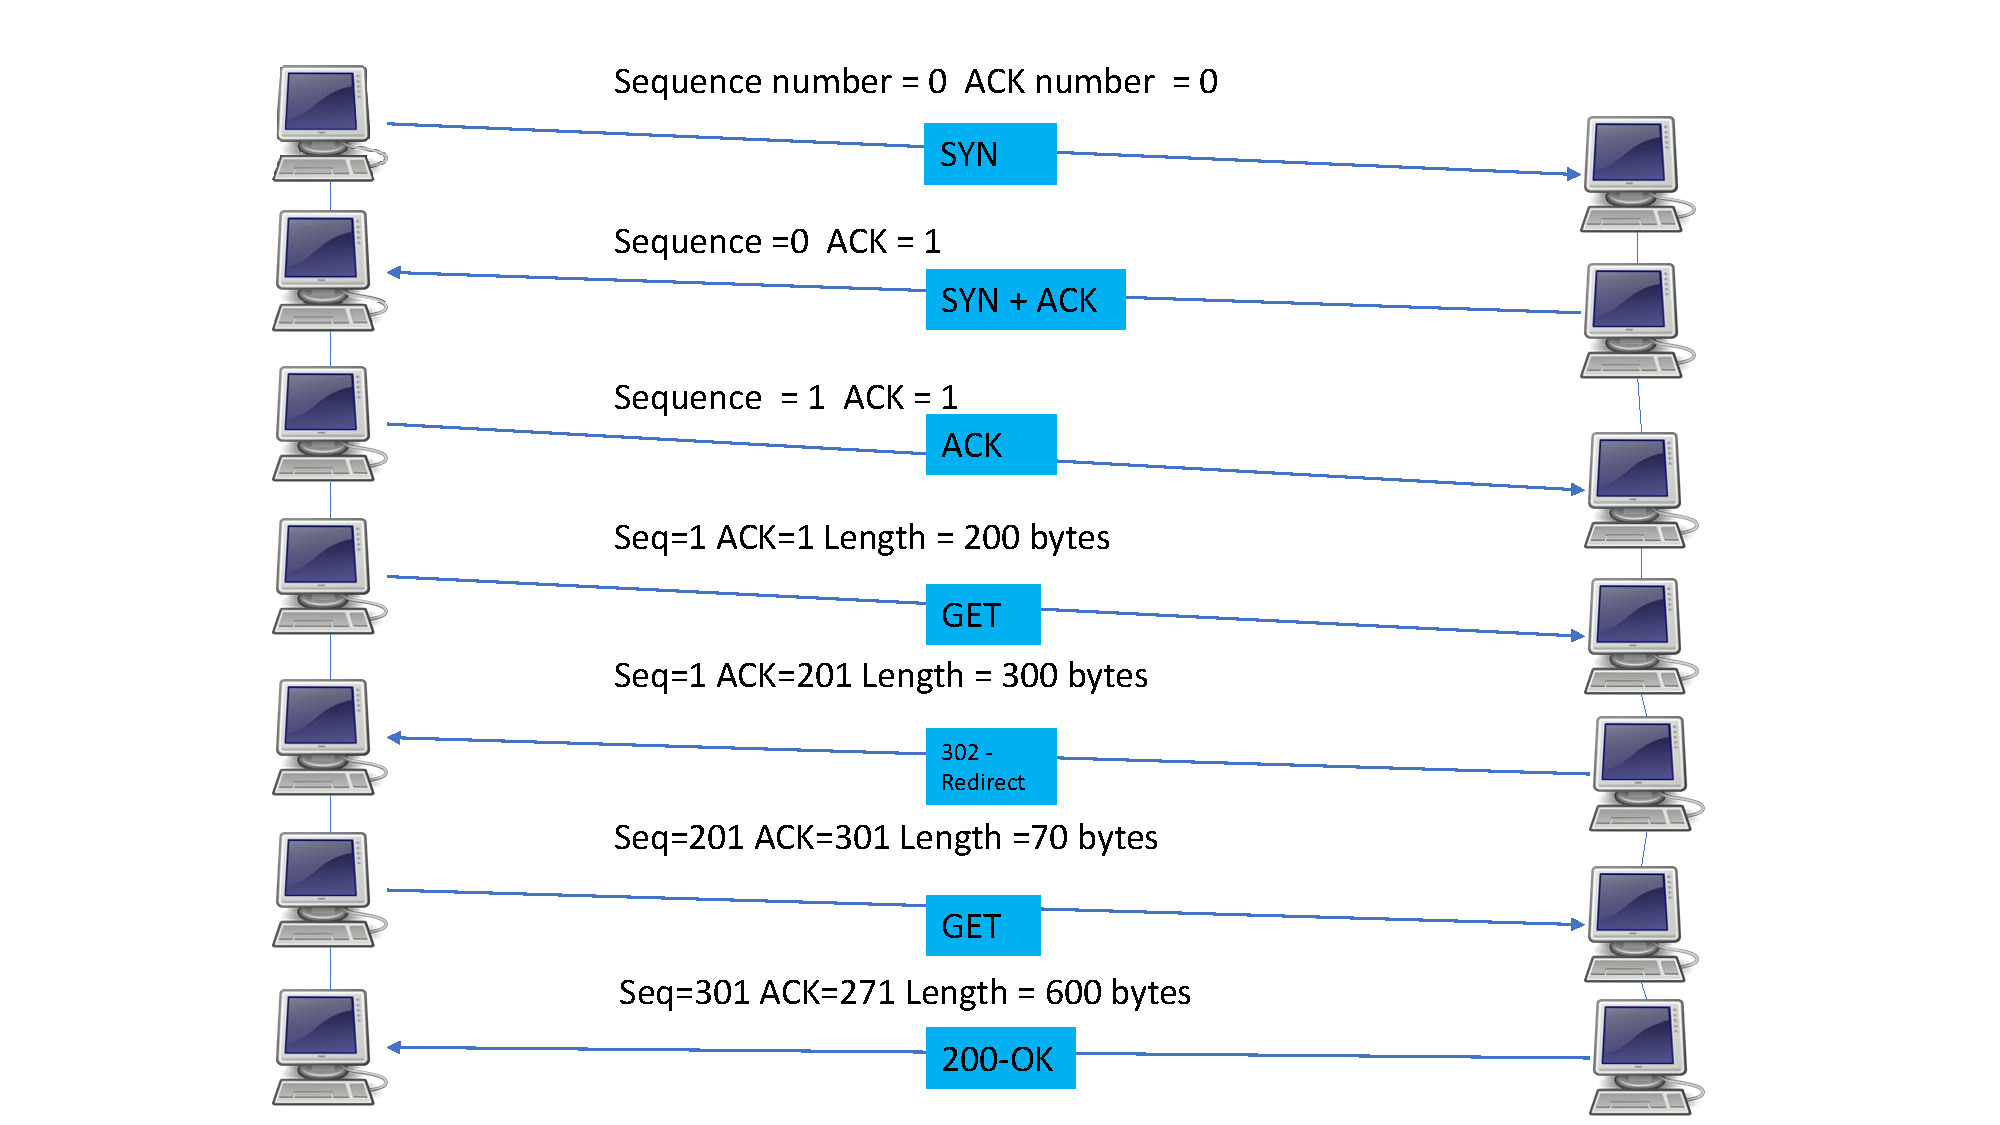
\includegraphics[width=0.87\textwidth]{ACK.pdf}
    \caption{TCP Relationship between SEQ and ACK where the response ACK = previous SEQ + Payload in bytes}
    \label{fig: TCP SEQ + ACK} 
\end{figure}

This completes this section on our methodology for development and implementation of our PEP. The next chapter will focus on our experimentation with the PEP in the University of Auckland Pacific Island Satellite Simulator. The chapter will report on the results found and will compare the findings with results found when PEPsal was tested on the Pacific Island Satellite Simulator by a Phd Student of University of Auckland. 

% chapter 5:  Jitter
\chapter{FINDINGS}
\begin{figure}[ht!]
    \centering
    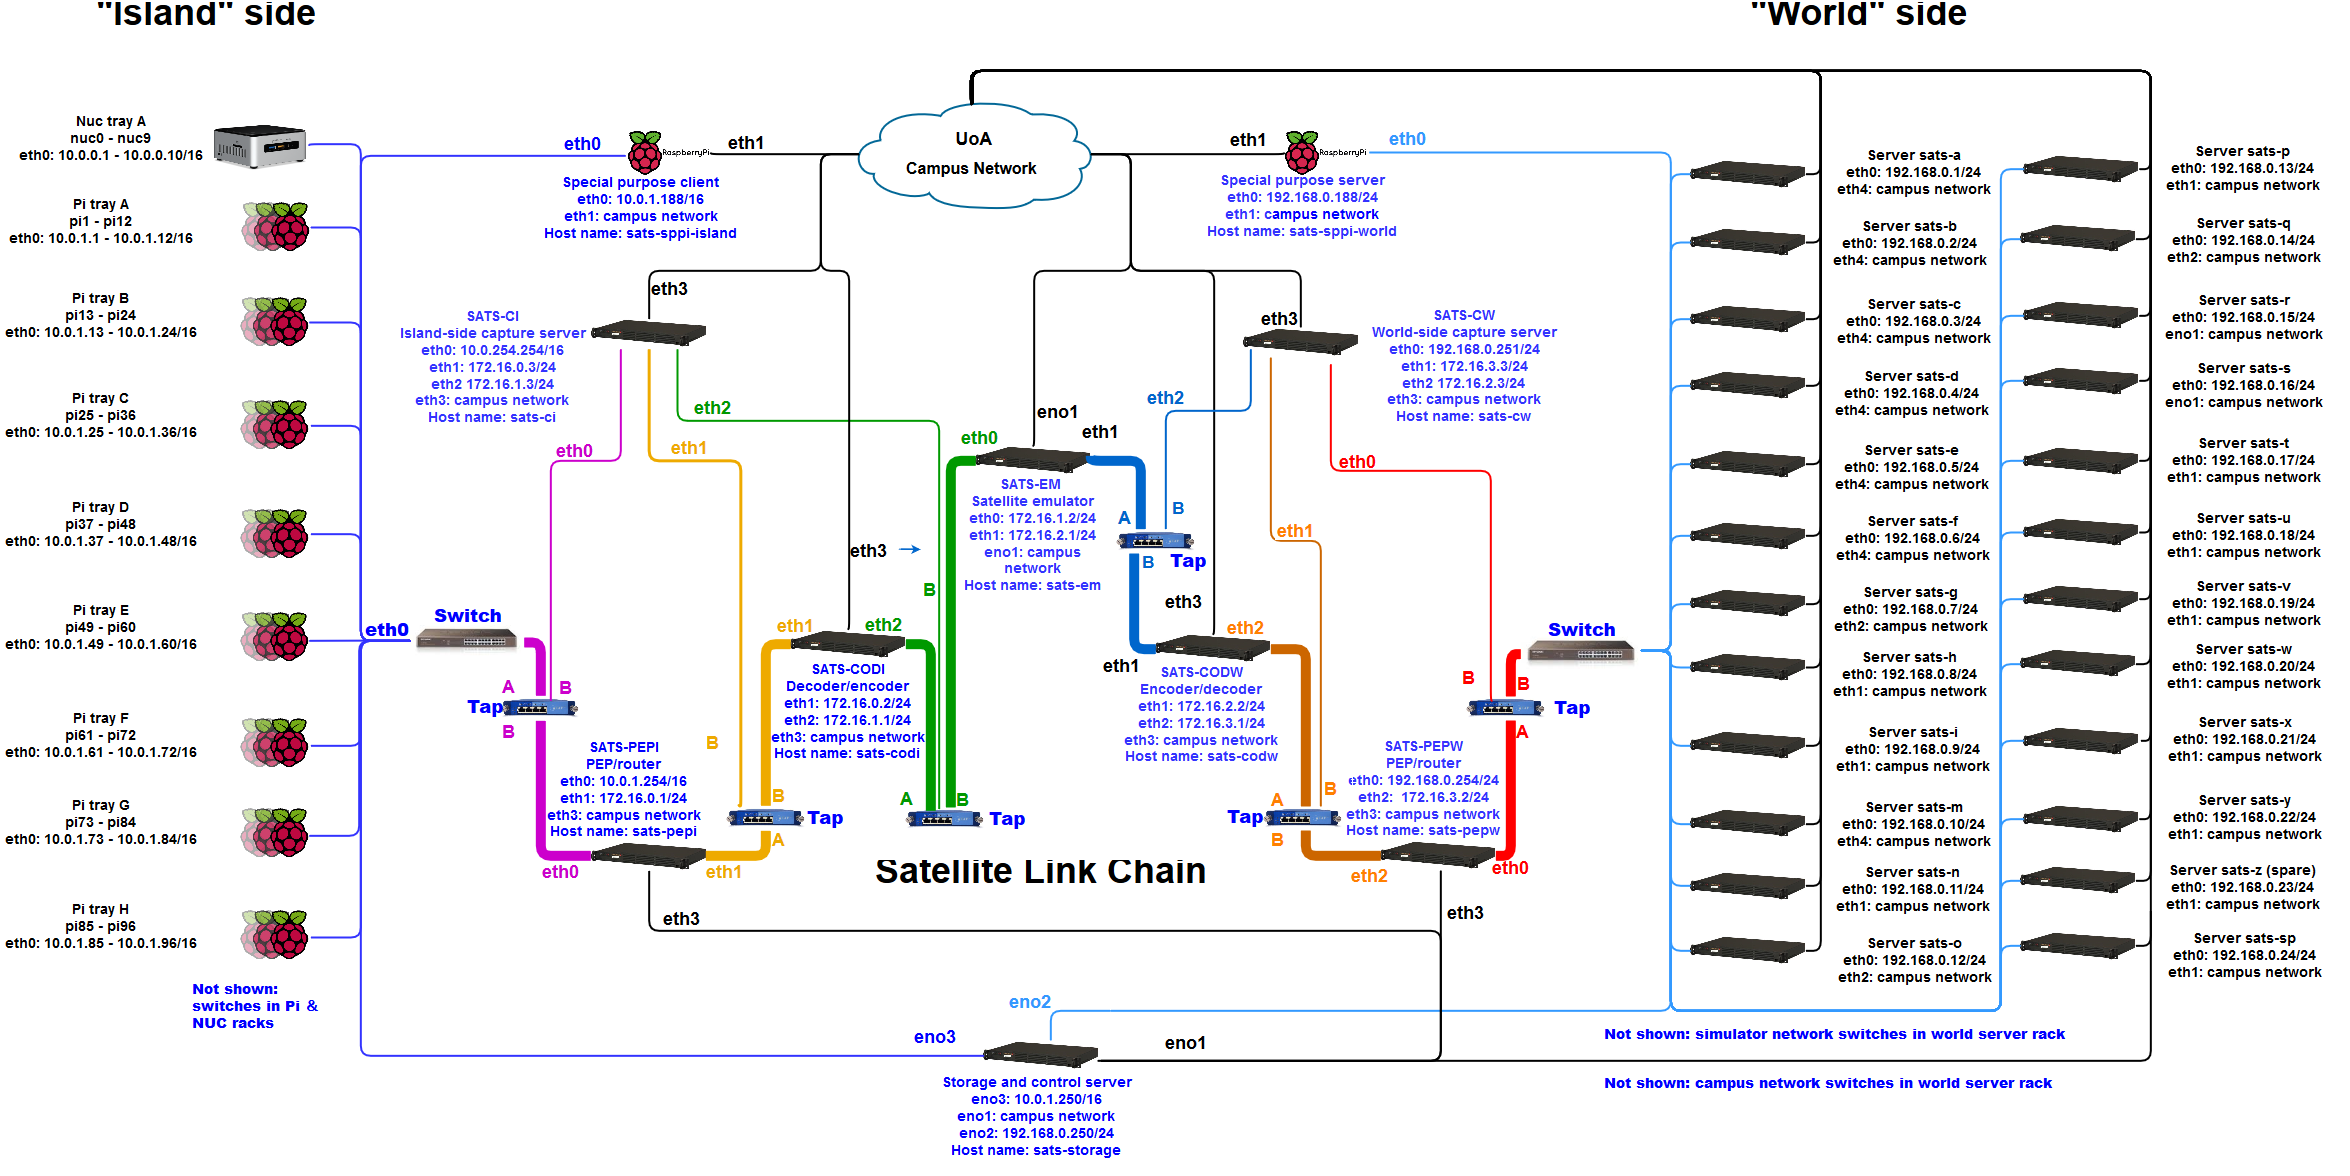
\includegraphics[width=1.3\textwidth, angle =270]{Simulator.png}
    \caption{Pacific Island Satellite Simulator Topology. }
    \label{fig: Satellite Simulator} 
\end{figure}

This section will be looking at the findings when we tested the PEP on the University of Auckland's (UOA) Pacific Island Satellite Simulator. These findings are compared to the PEPsal results conducted previously obtained on the same testbed by a PhD student- Quan and Professor Speidel. The road to get to this testing stage, however, was paved with many challenges. Section ~5.1 will look at the Pacific Island Satellite Simulator testbed before we look at the testbed experiment results in Section 5.2 and discuss the positives and negatives. \todo{make sure the section headings align} \\

\section{Pacific Island satellite testbed}
Figure 5.1 shows the general topology of the simulator.The simulator consists, in principle, of four networks. These four networks are represented on Fig 5.1 by the four different line colours. Each machine connected via the same coloured line is part of the same network and can see all other machines on the network directly without the aid of a router ~\cite{21}. \\

\subsection{Simulator topology and the technology within the simulator}
The testbed is divided into two halves. On the left side, connected by the thin light blue lines/network, we have the island side which represents the terrestrial hosts on the Pacific island. This left-hand side of the testbed consists of 96 Raspberry Pis and a tray of mini NUC PCs with SSD and a small amount of memory. The NUCS and Raspberry Pis run on the light blue private network which can be seen to the left of the Pis in Fig 5.1. These machines are simulating the clients sitting on the island side that will be connecting and receiving data from the servers on the world side (right-hand side of the topology). Their job is not very computing intensive as they only need to record the amount of data received and the time it arrived, hence the use of raspberry pis and NUCs ~\cite{21}. \\

On the right side, connected by the thin dark blue lines/network, are the machines representing terrestrial hosts from the world side on the other side of the satellite link. This side consists of 24 devices acting as the servers of the world in the simulated "world" network. 22 of these machines are actively simulating servers of the world, 1 of them of them is a special purpose server, and the last one is a spare machine to be used in case one fails. Standard switches connect these machines. They will receive socket connection requests from the clients on the island side and reply with data ~\cite{21}. \\

Right in the middle near the centre of the page, we have the satellite emulator SATS-EM which represents the geostationary satellite providing Internet access from the world side to the island side. This machine (SATS-EM) simulates the bandwidth constraints and latencies of the narrowband satellite link. For example, on a 16Mbps geostationary satellite link, it ensures that the data rate going through is only 16Mbps as per the real link and simulates the satellites link latencies and queue input capacities to the satellite. The thick multicoloured lines running through the satellite (SATS-EM) from the left "island" side through to the right "world" side, represents the bottleneck satellite link chain. This chain contains four further machines that by default are all configured to act as forwarding routers unless they are given a specific task ~\cite{20}~\cite{21}.\\

SATS-PEPI is the \emph{island-facing router/PEP} machine connected by the thin light blue lines to the left-hand side, and SATS-PEPW is the \emph{world side facing router/PEP} connected by the thin dark blue lines to the right-hand side. While the simulator allows for PEPs to be set up in a distributed architecture on both sides of the degraded satellite link, only the \emph{world side facing router/PEP} is being used as a performance enhancing proxy ~\cite{4}~\cite{5}~\cite{21}. The SATS-PEPI can be treated as a standard vanilla router for forwarding traffic in our case (integrated architecture). The reason for this is because in our experiments, practically all of the traffic payload data will be coming from the world-side to the islands hosts so there is no benefit from having a PEP configured on the island side ~\cite{21}. This has been configured this way just for ease of experimentation measurements but in a real world scenario, we would use a distributed architecture. The two switches between the PEPs and their island sides/world sides are simulating ground station equipment.\\ 

Between the PEPs and the SATS-EM (satellite emulator), we have two machines SATS-CODI and SATS-CODW which are decoders and encoders for network coding. Our experiments do not use network coding, so they act as plain vanilla routers in this case. We also have six copper taps along various points of the satellite link. They are used to capture and copy traffic and feed data directly to server SATS-CI  (island-side capture server) and SATS-CW (world-side capture server) for processing, shown in Figure 5.1 via the thin multicoloured lines ~\cite{20}~\cite{21}. \\

Right at the bottom of Figure 5.1, towards the centre of the diagram, is the storage and control server which controls the experiment. It is connected to the campus network via the thin black lines in the picture. The campus network sits outside our simulated satellite network so we can make configuration/software changes and check the experiments externally. This external access allows for changes to be made to the operation and for interaction with the world side servers without causing interference to the test ~\cite{21}. \\

Finally, we have the two Raspberry Pis located at the top of Figure 5.1 that act as two special purpose client and server Pis. These Pis send ICMP pings at the start of the experiment and then again at the end. These pings are visible in all traces taken along the satellite chain. When the PEP processes the data, these pings identify the start and end of an experiments captured data for better data analysis accuracy ~\cite{21}. 

\subsection{Basic rundown of the experiment}
On the island side, we have a client program that is run on the NUCs and the Raspberry Pis. This program involves the use of \emph{channels} which are defined as TCP socket connections that are repeatedly made between a client on the island side to a randomly selected server on the world side in a sequential order. We configure each client program with a certain number of these channels. A count is done on all the channels configured for all the NUCs and Pis and this allows us to control the load on the satellite link. Once the connection has been made, the server sends the island-side client a certain amount of data (as determined by the sender from a known flow size distribution collected from the Cook Islands) and then the socket connection is ended. The client channel then repeats the process and opens a new TCP socket connection to another randomly selected server. This process is repeated until the experiment times out ~\cite{21}. \\

The special purpose server (SATS-SP) located on the world side has a special purpose in our experiment. Since our clients randomly select the servers and the amount of bytes the servers send back to the clients is also randomly selected, it is possible only to get small or medium size transfers. The SATS-SP guarantees we get a large size transfer across our simulated network link. When the experiment starts, the SATS=SP connects to an iperf3 server on one of the NUCs and then transfers a significant amount of data ~\cite{21}. In our experiment, this nominal transfer is 40MB. \\

The SATS-SP also pings continuously at the start of the experiment, at rate of ten times per second. The ping packets are ideal because they are accepted into the byte queue at the input of the satellite link, even when the link is congested and the queue is overflowing with larger packets. Their tiny size means they can squeeze in at the end of the queue where larger data packets cannot ~\cite{21}.\\

The following is a basic rundown of the experiment procedure:

\begin{enumerate}

\item Test the system. Test the connectivity to make sure all servers can be pinged. We control the experiment via the external campus network so as to not contaminate the experiment traffic (storage and control server). 
\item Compute how we are going to distribute the requested number of channels among the Pis and NUCs. Automatically generates a script which starts up the Pis and NUCs and shuts them down.
\item Start capturing at the tap nearest the island-side and continue along the rest of the taps. The idea is that any data/packets captured at one tap and not showing in the next one can be assumed lost somewhere along the satellite chain. Start capturing at the tap nearest the world side. 
\item Start the world servers then start the clients (island-side). Let them both ramp up for ten seconds.
\item Start the iperf3 server on one of the NUCs. Note that in iperf3, the client sends data to the server rather than downloading it.
\item Send special client ping after ten seconds to signal the start of the experiment.
\item Start pinging and iperf3 transfer. Each experiment will run for approximately 600 seconds. (120 experiments will run in one batch).
\item  The special server world-side sends an \emph{end} pings after approximately 600 seconds of experiment time.
\item Shut down the iperf3 client, island clients and world servers.
\item Retrieve trace files collected by the taps from both capture servers and the iperf and ping logs from the world side special purpose server.
\item Collect data analysis from storage server and render onto graph.\\
\end{enumerate}

In the next section, we look at three different graphs yielded from three different batches of these experiments. Each batch contains 120 individual experiments which take roughly 15 to 30 minutes each to perform. We ran the experiments with load levels of between 10 to 120 channels and for each load level we ran 10 experiments ~\cite{21}. \\

We will perform the same batch of experiments on three different variations of our PEP. The only difference will be in the PEP input queue capacity and its retransmission times as can be seen in the next section.\\

For each of these three experiments, there was already an existing dataset of equivalent baseline and PEPsal experiments that we are using for comparison here ~\cite{4}~\cite{21}. 

\section{Running the PEP on the Satellite Simulator}
In the three graphs presented in this section, we have three data series in each graph as represented by three colours. Black represents baseline (no PEP), blue represents PEPsal, and the red the results of our PEP. The x-axis represents the client load we are putting on the link, measured in channels. The left y-axis marked with crosses represents total goodput. \\


\begin{figure}[ht!]
    \centering
    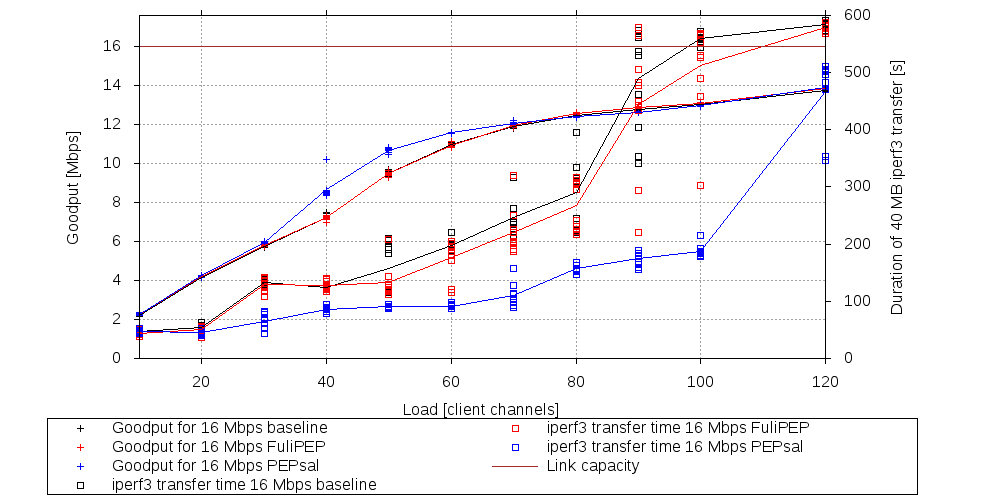
\includegraphics[width=1.3\textwidth, angle =270]{120K.png}
    \caption{Satellite link input queue capacity 120 kB, maximum RTT estimated as 1.3 * measured RTT of last ACK.}
    \label{fig: 120K queues} 
\end{figure}

Normally, total goodput is defined as the rate by which \emph{useful data} traverses the link, but in our experiment, our simulator measures total goodput as the rate of TCP payload data arriving at the other end of the link. Here, we want the total goodput to be as high as possible of course. \\

In the case of our PEP, this may include premature retransmissions, which normally would not be accounted for under goodput. However, due to the way the simulator operates and the fact that it is somewhat difficult to get the goodput from a large number of flows, we are constrained to having this as a possible adverse side effect. \\

Each individually coloured box represents the \emph{total iperf3 transfer} time for one experiment (y-axis). A good PEP result is when this transfer time is as low as possible indicating that data is capable of being transported faster across the link. The different coloured crosses represent the \emph{total goodput} for each experiment.\\

\begin{figure}[ht!]
    \centering
    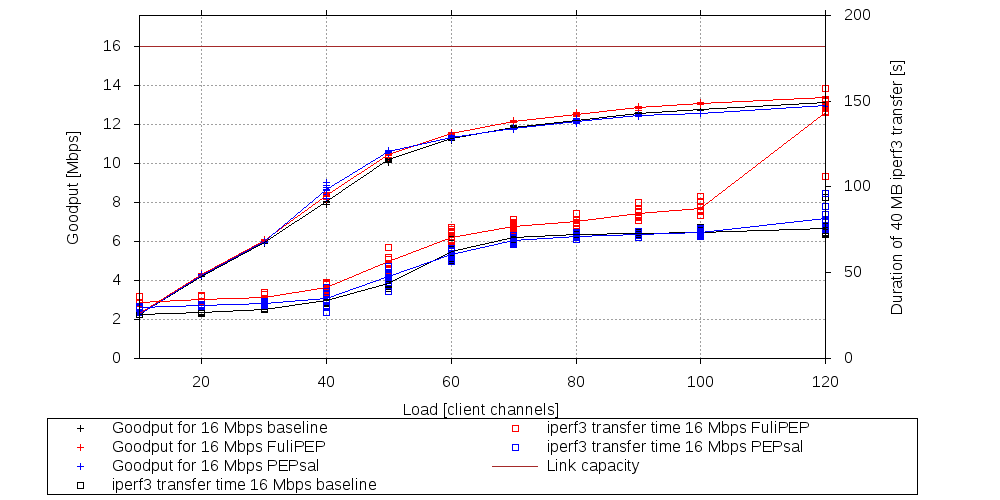
\includegraphics[width=1.3\textwidth, angle =270]{2000k.png}
    \caption{Satellite link input queue capacity 2000 kb, maximum RTT estimated as 1.3 * measured RTT of last ACK.}
    \label{fig: 2000k} 
\end{figure}

Figure 5.2 shows the results obtained from 120 experiments over varying loads when testing our PEP with a satellite link input queue capacity of 120k and a maximum RTT estimated as 1.3 x measured RTT from the last ACK. Recall that this dynamic recalculation of RTT affects the retransmission time for packets waiting in the cache. Hence the lower the multiple of RTT, the earlier our PEP will send retransmissions across the link. As mentioned above, however, this could affect the goodput in our experiment as it may result in more retransmissions.\\

We observe that the total goodput in our PEP is nearly identical to baseline (no PEP) and comparable to that of PEPsal except in the mid-load range between 30 and 70 client channels, where PEPsal is up to about 20 percent ahead.\\

For the individual iperf3 transfer, it is evident that our PEP performs better than baseline from about 50 client channels onwards, but it falls well below matching PEPsal's results just yet. Hopefully, our PEP will outperform PEPsal in the future once we can adjust the code to keep track of what is on the link and adjust the receiver's advertised window (rwnd) accordingly (see future work section in the next chapter).\\

\begin{figure}[ht!]
    \centering
    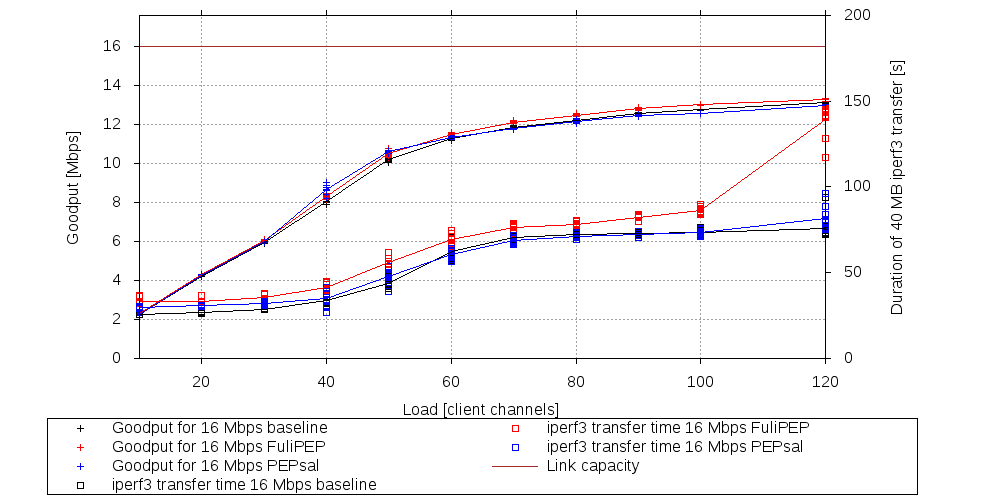
\includegraphics[width=1.3\textwidth, angle =270]{2000k-2.png}
    \caption{Satellite link input queue capacity 2000 kB, maximum RTT estimated as 2 * measured RTT of last ACK.}
    \label{fig: 2000k + 2*RTT} 
\end{figure}

Figure 5.3 shows the results obtained from 120 experiments over varying loads when testing our PEP with a satellite link input queue capacity of 2000kb (conventionally recommended queue capacity) and a maximum RTT estimated as 1.3 x measured RTT after last ACK. Total goodput, in this case, starts to slightly exceed PEPsal at around the 60 load channel mark and also performs above baseline across the board. While the PEP has an extra few percent of total goodput, some of this could theoretically be due to retransmission duplicates being counted as goodput (we only count TCP payload bytes), but if this is not the case, then the results are positive. For the individual iperf3 transfer, however, both the PEP and PEPsal have worse (more extended) transfer times than baseline. This will hopefully improve with future modifications to the PEP (see future work section in the next chapter). \\

Figure 5.4 shows the results obtained from 120 experiments over varying loads when testing our PEP with a satellite link input queue capacity of 2000kb (conventionally recommended queue capacity) and a maximum RTT estimated as 2 x measured RTT after the last ACK. The results are almost exactly identical to the previous experiment in Figure 5.2. From this result, we can tentatively conclude that the goodput is being measured accurately because the changes made to estimated RTT and the subsequent frequency of retransmissions have seemingly no effect on the results. If the retransmissions were a significant part of the goodput, we would expect to see a markedly different result when we change from 1.3 x RTT to 2 x RTT. The link input queue capacity seems to be the only variable in these three graphs that makes a discernible difference to the results. 
% chapter 6: Estimating of Network Quality, Voice Quality, and Buffer Requirements
\chapter{CONCLUSIONS}

\section{Research summary}
In conclusion, given the time constraints and challenges encountered during the creation of the PEP, the non-connection breaking PEP worked adequately in the sense that it permits connectivity and in some cases shows improvement over baseline. In the experiments from the previous chapter, it is, for the most part, performing above the baseline with respect to goodput. When compared to PEPsal, our PEP is largely outperformed, especially with iperf3 transfer time. The non-connection breaking PEP does, however, show a slight improvement in total goodput with the 2000k input queues over the heavier loads (> 60 client channels) which is promising. With future modifications, we hope to improve the PEP performance considerably. \\

Upon analysing the weaknesses of the PEP, one self-critique that does stand out is that we could not make the non-connection breaking PEP do enough to counter the two main problems mentioned in chapter 4, that TCP splitting/connection breaking PEPs create when they break the fundamental end to end semantics of the Internet. IPsec and VPN connections are merely forwarded through, but they also do not benefit from improved link optimisations via our PEP. The "where is the money" problem mentioned in chapter 4, also does not get any real resolution from our PEP. Our PEP does, however, reduce the probability of this problem occurring, only because it does more forwarding and less proxying/spoofing than a connection breaking PEP. This PEP could arguably be improving on a connection breaking PEP because we could say that our non-connection breaking PEP provides a statistical benefit by reducing the chance of that problem occurring. Such a claim may be hard to quantify so further testing in the future would be needed to confirm it.

\section{Future Work}
The good news is that there is much room for improvement on our PEP. Many aspects of the PEP logic could not be implemented due to time constraints. The author believes that the following modifications could make a significant improvement to our PEPs performance:\\

\subsection{Manipulating the TCP flow control receiver window}

The author considers this the most important future development to aim for as it should make the largest difference to the performance of the PEP but which regretfully had to be omitted for this thesis for time reasons. We aim to compute a meaningful value for the receiver's advertised window that would reflect the bandwidth delay product (BDP) of the link. The BDP, as explained previously, represents the maximum number of bytes/data that can be in transit over the satellite link at a given time ~\cite{4}~\cite{13}. \\

Our current PEP configuration has a constant advertised window of 65535 bytes in any ACK the PEP itself transmits to a TCP sender. This renders the \emph{TCP flow control} receiver window (rwnd) mechanism ineffective. As a TCP congestion window (cwnd) on a connection opens, it will eventually contribute to overwhelming the link capacity of the input queue to the satellite link and any intermediate routers along the link path. The advertised window the sender sees from the remote receiver indicates no shortage of processing capacity. Future work on the advertised window via our PEP should allow us to control the amount the sender transmits by advertising a rwnd that keeps track of the data in flight on the satellite link, and thus is able to throttle the sender before it overloads the link ~\cite{17}~\cite{18}.

\subsubsection{Implementing the variable receiver window for flow control}
The general idea here is to build our own TCP flow control mechanism (see Section 2.2.1) within the PEP that can dynamically gauge the spare capacity we have left on the link and advertise this via a receive window (rwnd) in an ACK back to the senders. Note that this is only possible for us to do because we know that the receiver sits on an island and therefore the BDP on the island is determined by the satellite link bandwidth multiplied by the \emph{negligible delay} on the island ~\cite{4}. Thus the overall BDP is given more or less by that of the satellite link itself. This method would not work, for example,  with a satellite facing PEP managing a link between two large continents because we have significant terrestrial latencies on both ends ~\cite{5}.\\

We know that there will be multiple active connections and senders transmitting over the link so our PEP needs to be able to advertise a rwnd that reflects the total spare link capacity divided by number of active senders ~\cite{1}~\cite{2}. \\

Our existing PEP configuration has a function called {\tt processTxQueue()} which dequeues packets from an interface transmission queue (called txQueue) and transmits them via a socket send() function. \emph{Remember that for both our incoming and outgoing interfaces of our PEP, we have created a {\tt struct proxyInterface} that has a transmission queue ({\tt txQueue}) and a receive queue ({\tt rxQueue})}. Packets in the {\tt txQueue} are ready to be sent, (i.e. they have their next hop destination MAC address etc.) so they are passed to the {\tt send()} function and are also cached if they are TCP packets with a payload. \\ 

To help enable a variable receive window, we could add two additional functionalities to {\tt processTxQueue()}, which would be put on the PEPs satellite-facing interface only. These functions would make use of a simple FIFO queue (linked list) to help keep track of the packets the PEP is transmitting over the link (data/bytes in flight). We could use a smaller version of our existing {\tt struct packetQueueElement} (requires less memory) which we can call {\tt byteQueueElement} that has fields which only record the size of a packet and a timestamp as shown below. \\

\begin{lstlisting}
/* Buffer element in queue that holds a packet 
including Ethernet header */
struct byteQueueElement {
    uint16  packetSize;
    struct timeval insertTime;
    struct byteQueueElement* next;
};

/* FIFO (linked list) queue struct for packets in flight 
on the link */
struct bdpQueue {
    struct byteQueueElement* head;
    struct byteQueueElement* tail;
    int bytesInFlight;
};
\end{lstlisting}

We can also use a smaller version of our FIFO queue {\tt struct packetQueue} (see Appendix B) shown above as "{\tt bdpQueue}" which will help keep a tally of the data/bytes being sent out on the link. The basic concept behind this is that for every packet that our PEP sends towards the satellite link, we simultaneously enqueue a {\tt byteQueueElement}. It stores the packet size (in bytes) and records the time the packet is being sent. The {\tt bdpQueue} represents the link capacity with bdp being the acronym for \emph{bandwidth delay product}. The packets in the {\tt bdpQueue} thus represent the packets that are currently in flight, so the idea is that the byteQueueElements in the bdpQueue will represent the packets traversing the link at present.\\

We maintain a variable {\tt int bytesInFlight} within bdpQueue that is initially set to 0 and incremented, by the size in bytes, of each packet enqueued at the bdpQueue. Now, we add two functions that we can call from {\tt processTxQueue()} on the satellite facing interface: \\

The first function, which we can name {\tt checkByteQueueElement()}, will check the {\tt byteQueueElement} (if any) at the head of the {\tt bdpQueue}. If the element's timestamp is younger than the satellite link RTT, the function just returns. If the element's timestamp is older than the RTT, it dequeues the {\tt byteQueueElement} and deducts the value of its size field from {\tt bytesInFlight}. It then disposes of the {\tt byteQueueElement}. \\

The second function can be named {\tt makeByteQueueElement()}. The {\tt packetQueueElement} for the packet that has just been sent, is taken as a parameter for this function. A {\tt byteQueueElement} is then created with the size parameter set to the size of the packet from the {\tt packetQueueElement} and the timestamp is set to the current time. The {\tt byteQueueElement} is enqueued on the {\tt bdpQueue}. The size of {\tt byteQueueElement} is added to {\tt bytesInFlight} to represent the total number of bytes on the link.

We would call the {\tt checkByteQueueElement()} function first to see if any older packets need to be removed from the {\tt bdpqueue} right before we call {\tt send()} on any packet in {\tt txQueue}. We then call {\tt makeByteQueueElement()} immediately afterwards to add the record of that sent packet (size in bytes) originating from {\tt txtQueue}, to our {\tt bdpQueue}. Actioning these calls in this order, firstly ensures that the {\tt byteQueueElement}'s are removed from bdpQueue if they have been enqueued longer than RTT. Secondly, it allows us to add a {\tt byteQueueElement} bdpQueue for every packet we send out on the PEP. So we are recording the bdpQueue's size increments and decrements, by incrementing and decrementing our bytesInFlight value accordingly. Thus we obtain a relatively accurate estimate of the number of bytes currently in flight over the link (ignoring for a moment the possibility that some of them may be in packets that the satellite link input queue drops). 

Hence, using bytesInFlight, we can almost accurately gauge two likely scenarios on the link. Firstly, if our bytesInFlight value exceeds the link BDP (link bandwidth x RTT => Pacific island region BDP = 16Mbs x 500 ms = 1MB) which is roughly 1MB in our case, then we can probably assume that our satellite input queues may be overflowing. This would trigger the action in our code to stop our PEP from sending which at this time of writing is planned to be an advertised rwnd action (advertised rwnd of zero in this case) as mentioned earlier. \\

The second scenario is that our bytesInFlight is below than BDP so we can calculate the spare capacity on the link by subtracting the bytesInFlight value from the BDP. The difference is a number that denotes the amount of data the link could currently handle without getting overloaded. This spare capacity is what we want our PEP to advertise to the senders via rwnd. As there will usually be multiple senders at any one time across the link, we would need to distribute that spare capacity across our active connections. Otherwise, we will encounter the same congestion problems with the senders not having an accurate view of the link's capacity.\\

We propose to divide the spare capacity by the number of active connections to obtain a shared value. If the result is bigger than 65535, then we are content to keep our constant as it is. However, if not, we need to insert that shared value into the advertised window of the subsequent ACKs that our PEP sends out. \\

\textbf{Example:}\\

A typical BDP for a Pacific Island network reliant on a geostationary satellite for Internet and with a link rate of 16Mbps is 1 MB [4][5]. Let us suppose that the current bytes in flight value is 400,000 and we have 60 active connections. Then we can calculate a shared value for the rwnd as 400,000 bytes divided by 60 for a shared value of 10,000 per connection, which is < 65535. Therefore we would advertise a receive window of 10,000 in our reply ACKs.\\

This approach doesn't take into account that many connections would not transfer that amount by the time they have completed, so we can be a bit more generous with those that do.
 
 \subsection{Increasing the speed and efficiency of ARP table look ups}
At the moment our ARP table and TCP connection table and cache use binary search trees (BST) as the main data structure. In future implementations, we could look at a faster more efficient search data structure like self balancing binary search trees or heap/hash tables for instance [42][43]. \\

\subsection{Restructuring the cache FIFO packet queues}
We could restructure the cache so that each packet is stored with the expiry time as key in a max heap rather than a BST, with the root being the packet that needs to be retransmitted first. This should ease the housekeeping burden [43].

\section{Limitations of the study?}

The results of this research can be applied specifically to many parts of the Pacific Islands region and also has some general applicability to other remote locations, such as oil rigs, (cruise) ships or planes where multiple TCP users have to share the satellite link. This section will highlight the limitations of this study as they affect the ability to generalise the thesis results across a wider scope. The limitations are as follows:

\begin{enumerate}
\item This study only tested for simulated geostationary satellite links.  The results cannot be applied to communities connected via MEO satellites for Internet connectivity. 
\item The experiments run on the satellite simulator testbed only tested for links with 16 Mbps in both directions and not for other bandwidths. There may be some uncertainty on how the PEP would react to vastly different bandwidths. Note that this is not so much a limitation of the PEP as such but a result of limited availability of the simulator, which was also being used for other experiments not related to this thesis.
\item Implementation of the variable advertised window (rwnd) for our PEP had to be shifted to future work. This codebase is a platform for further development, so the variable rwnd will be a feature that can be added later to improve the PEP performance. 
\item The optimisation of the RTT estimation algorithm would have required many more experiments for a better result. Unfortunately, there was not enough experiment time available on the simulator within the time frame of the thesis.
\end{enumerate}

\section{Final summation and recommendations}

This thesis has presented the first Linux based non-connection breaking PEP approach that is designed specifically for the Pacific Island regions reliant on narrowband satellite link provided Internet. The PEP currently provides small goodput gains for long downloads and is intended as a platform for further ongoing development with future work. The ultimate goal was to provide an inexpensive open-source PEP solution/platform for satellite-dependent parts of the Pacific Islands region that has the added bonus of not violating the fundamental end to end semantics of TCP. This goal has been achieved to an extent, and future work modifications are planned to improve the PEP performance (See Future Work section). To summarise, the PEP in this thesis has:

\begin{itemize}
\item provided a platform for an affordable open-source Linux based non-connection breaking PEP tailored for the Pacific island environment.
\item provided a platform going forward to deal with the issues created by TCP splitting/connection breaking PEPs when they break the end to end semantics of TCP. 

Namely:

  \begin{enumerate}
   \item the inability to deal with encrypted TCP flows      (example: IPsec) or VPN 
   \item the issue of false acknowledgements. Recall the     "where is the money" problem mentioned earlier whereby the PEP acknowledges back to a sender that a particular transfer has been received by the intended target. A problem arises when there is a technical problem on the receiver side, and they do not get the data for some reason. The sender will then falsely believe that the data has been received by the target.
  \end{enumerate}

\item been successfully tested against PEPsal and baseline in the University of Auckland satellite simulator and shown to have small gains in goodput for long downloads.
\item been scheduled for future work to build on the non-connection aspect of the PEP.
\end{itemize}

\subsection*{Recommendations}
Further testing on the satellite simulator with different bandwidths, refinement of the RTT recalculation, as well as experimentation with other types of satellites  (example: MEO) will also be beneficial going forward. As explained in Section 6.1 of these conclusions, the full potential of the non-connection breaking aspect of this PEP has not been yet reached. At this stage of development, our non-connection breaking PEP partially addresses the concerns of breaking the fundamental end to end rule of the Internet. There is still room for improvement.





% Appendix
  \begin{appendices}

\chapter{First appendix}
  \section{IP Header Struct}
  Let us now look at the actual \textbf{iphdr struct:} \\
  
\begin{lstlisting}
struct iphdr {
 #if defined(__LITTLE_ENDIAN_BITFIELD)
     __u8    ihl:4,
                 version:4;
 #elif defined (__BIG_ENDIAN_BITFIELD)
      __u8    version:4,
              ihl:4;
 #else
 #error  "Please fix <asm/byteorder.h>"
 #endif
       __u8    tos;
       __u16   tot_len;
       __u16   id;
       __u16   frag_off;
       __u8    ttl;
       __u8    protocol;
       __u16   check;
       __u32   saddr;
       __u32   daddr;
        /*The options start here. */
};
\end{lstlisting} 

The struct uses the correct version number, which alternates between big endian and little endian depending on the machines architectural set up. (Note: This thesis assumes the concept  of little endian, big endian is known to the reader. If not, be aware that it is not crucial to the understanding of the thesis). 


  \section{TCPhdr Struct}

\begin{lstlisting}
 struct tcphdr {
         __u16   source;
         __u16   dest;
         __u32   seq;
         __u32   ack_seq;
 #if defined(__LITTLE_ENDIAN_BITFIELD)
         __u16   res1:4,
                 doff:4,
                 fin:1,
                 syn:1,
                 rst:1,
                 psh:1,
                 ack:1,
                 urg:1,
                 ece:1,
                 cwr:1;
 #elif defined(__BIG_ENDIAN_BITFIELD)
         __u16   doff:4,
                 res1:4,
                 cwr:1,
                 ece:1,
                 urg:1,
                 ack:1,
                 psh:1,
                 rst:1,
                 syn:1,
                 fin:1;
 #else
 #error  "Adjust your <asm/byteorder.h> defines"
 #endif  
        __u16   window;
        __u16   check;
        __u16   urg_ptr;
};
\end{lstlisting}


\subsection*{Brief recap of Binary Search Tree(BST)}
The Binary Search Tree(BST) data structure will provides an efficient way to store, search and retrieve data (IP to MAC address mappings in our case). As can be seen in the data struct node, we have a node struct that contains two other node structs pointers called "left" and "right". This "node within a node" recursive structure will give us a recursive algorithm which allows for searching time of O(h) worst case runtime complexity where h stands for the height of the tree. As can be seen in Fig 4.12, a BST structure has has at least O(log n) levels for n number of nodes. It will thus make O(log n) comparisons at a minimum to find a target node. This is ideal in terms of both speed and CPU efficiency, since we will be perusing through multiple ip addresses per second on the satellite link. 

\begin{figure}[h!]
	\centering
    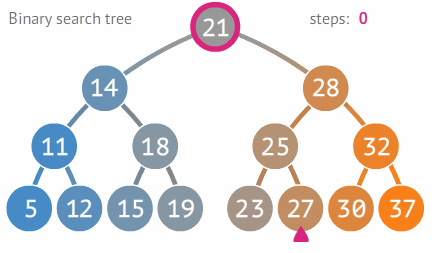
\includegraphics[width=0.87\textwidth]{BST.PNG}
    \caption{BST Structure}
    \label{fig:BST}
\end{figure}

In a standard BST structure the nodes are ordered as follows:

\begin{itemize}
\item each node contains one key (or data-in our case, our struct nodes key is "IP address" and its corresponding "MAC address" mapping is the nodes data).
\item the keys for a nodes left subtree are smaller than the key in its parent node.;
\item the keys for a nodes right subtree are bigger than the key in its parent node.;
\item Cannot have the same key in different nodes of the tree.\\
\end{itemize}

The writers assumption here is that Binary Search Tree algorithm is standard knowledge for the reader (if not, see section 2.3.4 "Topics to review"). Our PEP code incorporates the use of this BST structure to build our ARP Table cache. \\

\section{Challenges encountered}

Many unforeseen challenges encountered while creating the PEP coupled with the one year time constraints of a Masters thesis paper, hindered our ability to deliver a complete final product. In short, we did not have enough time to implement all of the proposed PEP logic planned for the PEP. The receiver window size (rwnd) as described previously in chapter 2 \emph{TCP flow control} was initially going to be a crucial part of our PEP. One of our aims for this project was to create a PEP where we could dynamically alter the receiver window size to adjust for congestion and idleness on the degraded bottleneck satellite link. This facet of the PEP, however, will be implemented as future work to improve the performance of the PEP. More detail will be provided in the next chapter on how this will work with our current PEP implementation.

\subsection{Kernel overriding code interface commands}
One problem that had not been anticipated was the kernel overriding code interface commands. We had coded our packets to be forwarded out a specific interface on our PEP via raw socket programming commands. The kernel, however, was calculating the best path and forwarding the packet out the interface it deemed best to suit that path. The interface chosen by the kernel was not always the one we had selected as the packets exit point (but quite often it was which aided the confusion), so it took some lengthy debugging time before being able to isolate the cause of the problem. A complete overhaul of the code was needed as we realised we would need to use struct sockaddr\textunderscore ll (see Appendix B) \todo{promise} for portions of our code, where it had not been previously, to reach into data link layer to override the kernel. 
In most socket programming applications, one can leave the assembly of Ethernet and IP header to the kernel. In raw socket programming, we can leave the assembly of Ethernet, as well as ARP requests for next-hop forwarding to the kernel. In our case, however, we need to spoof ACKs - and this means using a sender IP address that is not that of the interface we are sending from. This necessitates the use of sockaddr\textunderscore ll. 

\subsection{Creating own ARP requests and ARP tables for next hop forwarding}
Another issue involved having to create our own ARP table, and ARP requests to enable us to retrieve the destination MAC address for packets we wanted to forward (up until this point, our code had been hardcoding the destination Mac address to make our testing smoother). This required code that could assemble (and then send) an ARP request packet based on the IP address we receive from the sniffer and read the ARP reply we get back from the relevant target host to whom the IP address belonged. This task involved the use of our own customised binary search tree ARP cache table for our PEP to store a record of IP address to MAC mappings found.  \\

Alternatively, rather than handling the address resolution ourselves, we could have chosen to use a call to the popen() function, which we could have used to execute the ARP command and then parse its output. The problem, however, is that the \emph{popen()} function starts a new separate process and we could be calling this function quite often depending on the size of the local subnet that the PEP is directly connected to and the number of active hosts in that subnet we would have needed to resolve. Opening multiple additional processes in a time-critical environment, such as our PEP, would have adverse effects on performance, so the \emph{popen()} option was abandoned. \\

\subsection{Fine tuning ARP responses via non-blocking sockets}

Late into the coding process, we inadvertently discovered that we had what turned out to be a significant problem in that we were using the incorrect type of sockets. We stumbled upon this discovery while trying to fine tune our reception of ARP responses. Our current code would send out an ARP request on the forward interface, and our PEP would listen for the corresponding ARP response. If for instance, however, we never get an ARP response because the IP is local, but there is no such host on the network, the {\tt recv()} socket function will automatically \emph{block}. In other words, the {\tt recv()} function will not return until it has received a packet. Since there is no packet coming, the PEP will wait forever and stall. During this time, none of the other code executes, so we can not receive packets on the incoming interface, or perform any other actions in the PEP. The solution was to have a look at non-blocking sockets. Up until this point, we had used the standard raw sockets programming which blocks by default, so this required another code overhaul. \\

In short, non-blocking sockets does as its name suggests. They are sockets that do not block, so when we call {\tt recv()} or any other send or receive function and pass the socket as a parameter, that function will always return whether it receives a packet or not. The positive here is that this means the absence of packets will not cause our PEP to freeze, but the negative side is that it requires more code to check whether the {\tt recv()} function actually received a packet or whether it returned an empty value. \\

It eventually became apparent that the non-blocking sockets were not just crucial to the correct operation of the ARPing process, but they were in fact, also the critical element to building our PEP. In theory, the PEP needs to listen on its incoming and outgoing interfaces simultaneously. In practice, this is not possible as the socket programming has limitations that only allow it to listen on one interface at a time consecutively, although it can swap between the two interfaces at such high-speed that would make it seem almost simultaneous. While we were using the standard default blocking sockets, however, we might start listening on the one interface, but the receive function would not return until we had a packet arriving there (which could take forever, literally). Meanwhile, we might miss many packets on the other interface. Non-blocking means that if there is no packet pending on an interface, the function returns anyway (but empty-handed), so we can go on to check the other interface.

\subsection{Unavailability of the Satellite Simulator}

The University of Auckland Pacific Island Satellite Simulator was being used extensively for PhD experiments, so it was not available for use with this PEP until late January. 

\begin{figure}[h!]
    \centering
    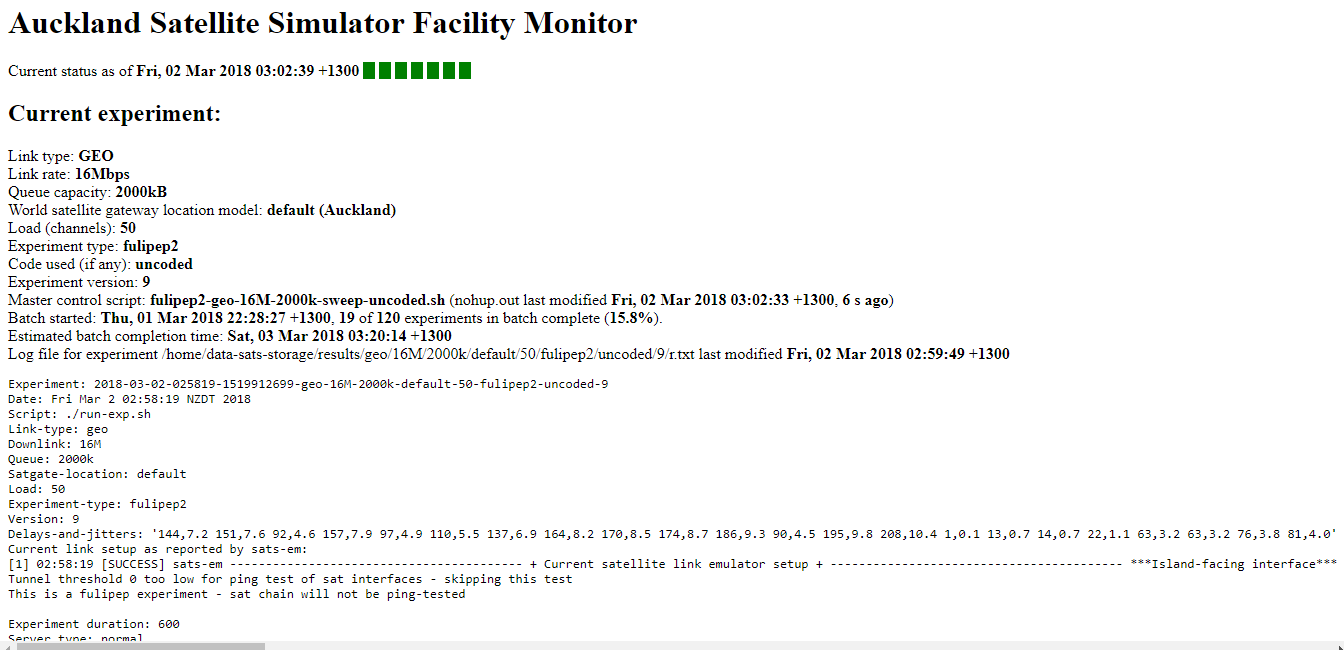
\includegraphics[width=0.87\textwidth]{experiment.PNG}
    \caption{University of Auckland Pacific Island Satellite Simulator Facility Monitor}
    \label{fig: experiment} 
\end{figure}

On top of that, we also had to deal with the following issues when preparing our PEP for the simulator.\\
\begin{enumerate}
\item Having to modify the experiment harness to be able to test it. That is: create startup scripts to start and stop the PEP on the PEP machine and remotely from the simulator's control machine. 
\item Adapting test scripts so they could accommodate the PEP, which includes changing experiment control files to create a new subtree for the log files for the PEP experiments, plus many smaller changes to analysis files.
\item Having to modify the proxy so it would forward ICMP and other non-TCP protocols directly as the simulator uses these during measurements. \\
\end{enumerate}
\todo{reword later as these are Ulrichs words}

Testing of the PEP required integration into the experiment harness of the simulator. This requirement was only possible after completion of the standard baselines and PEP experiments in late January. To do so, the PEP had to be modified to forward any non-TCP packets destined for the other side of the PEP. Some of your PEP's characteristics also required aspects of the experiment's harness quality control checks to be changed. These alterations took a couple of weeks to complete. \\

Last but not least, we had to test both for the "classic" 2000 kB satellite input queue capacity and for the 120 kB capacity we now recommend. \todo{(see \& cite https://application.isif.asia/theme/default/files/ISIFAsia\textunderscore 2016\textunderscore Grants\textunderscore TechReport\textunderscore UoA\textunderscore SimulationSatPAC.pdf, page 10/11)}
The results from each individual graph seen in the next section take about a week to complete as it runs its set of 120 experiments per graph. Only one set of experiments can be run on the simulator at any one time. The late access to the simulator plus the two-week simulator preparation and the time it takes for each set of experiments to run, left little room for major code changes and adjustments. \\

We also had the option of testing our PEP on an open source software based satellite network simulator like ns-2 or ns-3, but it would not be able to simulate the conditions of a Pacific Island satellite environment accurately. Our testbed is built specifically for the Pacific Island environment.\\

There are a few other limitations with these software simulations that we felt made its ability to simulate realistic network behaviour questionable:\\

\begin{itemize}
\item The software simulator uses an artificial timebase which limits the use of built-in network functionality.
\item Simulating many terrestrial latencies under high load is memory-consuming (because the simulator has to store all packets in flight)
\item Simulating a realistic mix of flow sizes is difficult. Many software simulations in the literature assume that it's enough to demonstrate that something gives a benefit if you load a link with a small number of long TCP flows (which are simulated as FTP most commonly, which is a sparsely used protocol these days).\\
\end{itemize}

\chapter{Second appendix}

The sockaddr\textunderscore ll structure is a device-independent physical-layer address ~cite{35}~\cite{44}.

\begin{lstlisting}
struct sockaddr_ll {
    unsigned short sll_family;   /* Always AF_PACKET */
    unsigned short sll_protocol; /* Physical-layer protocol */
    int            sll_ifindex;  /* Interface number */
    unsigned short sll_hatype;   /* ARP hardware type */
    unsigned char  sll_pkttype;  /* Packet type */
    unsigned char  sll_halen;    /* Length of address */
    unsigned char  sll_addr[8];  /* Physical-layer address */
};
\end{lstlisting}
\end{appendices}

\renewcommand{\baselinestretch}{1}
%\bibliographystyle{ieee}
\begin{thebibliography}{99}
%----------------------------------------------------------------------------------------
%	BIBLIOGRAPHY
%----------------------------------------------------------------------------------------

\bibitem{1} Lin, Y., Hwang, R. and Baker, F. (2012). Computer networks. New York, NY: McGraw-Hill. 

\bibitem{2} B. Forouzan, Data communications and networking. New York: MacGraw-Hill, 2013.

\bibitem{3} "Here's how a tiny Pacific island got better Internet than the US", Public Radio International, 2018. [Online]. Available: https://www.pri.org/stories/2014-08-01/heres-how-tiny-pacific-island-got-better-internet-us. [Accessed: 21- Mar- 2018].

\bibitem{4} U. Speidel, E. Cocker, P. Vingelmann, J. Heide and M. Medard, "Can network coding bridge the digital divide in the pacific?", 2015 International Symposium on Network Coding (NetCod), 2015.

\bibitem{5} U. Speidel, L. Qian, ’. Cocker, P. Vingelmann, J. Heide and M. Médard, "Can Network Coding Mitigate TCP-induced Queue Oscillation on Narrowband Satellite Links?", Wireless and Satellite Systems, pp. 301-314, 2015.

\bibitem{6} Border J, Kojo M, Griner J, Montenegro G, Shelby Z. “Performance Enhancing Proxies Intended to Mitigate Link-Related Degradations”, IETF RFC 3135, June 2001.

\bibitem{7} Y. Hu and V. Li, “Satellite-based internet: a tutorial”, IEEE Commun. Mag., pp. 154-62, March. 2001.

\bibitem{8} C Partridge, T Shepard, "TCP Performance over Satellite Links", IEEE Network, vol. II, no. 5, pp. 44, September 1997.

\bibitem{9} G. Xylomenos, G.C. Polyzos, P., Mahonen, and M. Saaranen, “TCP performance issues over wireless links” IEEE Commun.Mag., vol. 39, pp 52-58, April 2001.

\bibitem{10} M. Marchese, “TCP/IP-Based Protocols Over Satellite Systems: A Telecommunication Issue,” in Reliability, Survivability and Quality of Large Scale Telecommunication Systems, P. Stavroulakis, Ed. Chichester: Wiley, 2003, pp. 167-198.

\bibitem{11} K. Scott, P. Feighery, B. Crow and M. Jurik, “TCP congestion control in shared satellite environments”, MILCOM 2002 - IEEE Military Communications Conference, no. 1, October 2002, pp. 46 – 50.  

\bibitem{12} D. E. Comer, Internetworking with TCP/IP, Vol. I: Principles, Protocols and Architecture, 2nd ed., Prentice Hall, 1991. 

\bibitem{13} Partridge, C. and Shepard, T. (1997). TCP/IP performance over satellite links. IEEE Network, 11(5), pp.44-49.

\bibitem{14} Caini, C., Firrincieli, R. and Lacamera, D. (2007). PEPsal: A Performance Enhancing Proxy for TCP Satellite Connections [Internetworking and Resource Management in Satellite Systems Series]. IEEE Aerospace and Electronic Systems Magazine, 22(8), pp.B9-B16.

\bibitem{15}  Thanthry, N., Deshpande, M. and Pendse, R. (2006). A Novel Mechanism for Improving Performance and Security of TCP Flows over Satellite Links. Proceedings 40th Annual 2006 International Carnahan Conference on Security Technology.

\bibitem{16} M. Allman et. al., " Ongoing TCP Research Related to Satellites", RFC 2760, February 2000 

\bibitem{17} Allman M, Blanton E, Paxson V. “TCP Congestion Control”, IETF RFC 5681, September 2009. 

\bibitem{18} Stevens W. “TCP Slow Start, Congestion Avoidance, Fast Retransmit, and Fast Recovery Algorithms”, IETF RFC 2001, January 2001. 

\bibitem{19} V. Jacobson, "Congestion avoidance and control", ACM SIGCOMM Computer Communication Review, vol. 25, no. 1, pp. 157-187, 1995. 

\bibitem{20} U. Speidel, "Striking a balance between bufferbloat and TCP queue oscillation | APNIC Blog", APNIC Blog, 2018. [Online]. Available: https://blog.apnic.net/2018/03/19/striking-a-balance-between-bufferbloat-and-tcp-queue-oscillation/. [Accessed: 20- Mar- 2018].

\bibitem{21} "Auckland Satellite TCP/IP Traffic Simulator | Home of the Satellite TCP/IP Traffic Simulator at the University of Auckland", Sde.blogs.auckland.ac.nz, 2018. [Online]. Available: http://sde.blogs.auckland.ac.nz/. [Accessed: 25- Mar- 2018].

\bibitem{22} Z. Liu eta/., "Evaluation of TCP Vegas: Emulation and Experiment," Proc. ACM SIGCOMM '95, Aug. 1995, pp. 185-1 96.

\bibitem{23} J. C. Hoe, "Improving the Start-up Behavior of a Congestion Control Scheme for TCP," Proc. ACM SIGCOMM '97, Aug. 1996, p 270-280 

\bibitem{24} M. Mathis and J. Mahdavi, "Forward Acknowledgment: Refining TCP Congestion Control," Proc. ACM SIGCOMM '96, Aug. 1996, pp. 281-291.

\bibitem{25} L. S. Brakmo, S. W. OMalley, and L. L. Peterson, "TCP Vegas: New Techniques for Congestion Avoidance and Control," Proc. ACM SIGCOMM '94,
Aug. 1994, pp. 24-35.

\bibitem{26} C. Caini and R. Firrincieli, “TCP Hybla: a TCP Enhancement for Heterogeneous Networks”, International Journal of Satellite Communications and Networking, vol. 22, n. 5, Sep. 2004, pp. 547-566.

\bibitem{27} C. E. Palazzi, C. Roseti, M. Luglio, M. Gerla, M. Y. Sanadidi, and J. Stepanek, “Enhancing Transport Layer Capability in HAPS-Satellite Integrated Architecture”, Wireless Personal Communications, Springer Science+Business Media B.V. (formerly Kluwer Academic Publishers B.V.), vol. 32, no. 3-4, Feb 2005. 

\bibitem{28} D. Velenis, D. Kalogeras, and B. Maglaris, “SaTPEP: a TCP Performance Enhancing Proxy for Satellite Links,” 2nd International IFIPTC6 Networking Conference, May 2002. 

\bibitem{29} "US6975647B2 - Enhancements for TCP performance enhancing proxies - Google Patents", Patents.google.com, 2018. [Online]. Available: https://patents.google.com/patent/US6975647B2/en. [Accessed: 25- Mar- 2018].

\bibitem{30} A. Bakre, B. R. Badrinath, “I-TCP: Indirect TCP for Mobile Hosts”, Proc. 15th IEEE International Conference on Distributed Computing Systems, Vancouver, British Columbia, pp. 136-143, May 1995. 

\bibitem{31} R. Yavatkar and N. Bhagawat, “Improving end-to-end performance of TCP over mobile internetworks”. IEEE Workshop on Mobile Computing Systems and Applications, pages 146--152, December 1994. 

\bibitem{32} T.R. Henderson, and R.H. Katz, “Satellite Transport Protocol (STP): An SSCOP-based Transport Protocol for Datagram Satellite Networks”, 2nd International Workshop on Satellite-based Information Services (WOSBIS `97), Budapest, Hungary, Oct. 1, 1997. 

\bibitem{33} "GregoireDelannoy/TCPeP", GitHub, 2018. [Online]. Available: https://github.com/GregoireDelannoy/TCPeP. [Accessed: 25- Mar- 2018]. 

\bibitem{34} Artes.esa.int, 2018. [Online]. Available: https://artes.esa.int/sites/default/files/FastSatDataSheet\textunderscore 1.5.pdf. [Accessed: 25- Mar- 2018]. 

\bibitem{35} S. Walton, Linux socket programming. Indianapolis]: Sams, 2008. 

\bibitem{36} "packet(7) - Linux manual page", Man7.org, 2018. [Online]. Available: http://man7.org/linux/man-pages/man7/packet.7.html. [Accessed: 26- Mar- 2018]. 

\bibitem{37} "IBM Knowledge Center Error", Ibm.com, 2018. [Online]. Available:https://www.ibm.com/support/knowledgecenter/en/SSLTBW\textunderscore 2.3.0/com.ibm.zos.v2r3.cbcpx01/ovsock.htm. [Accessed: 26- Mar- 2018].

\bibitem{38} A. Sockets and S. Saxena, "A Guide to Using Raw Sockets", Open Source For You, 2018. [Online]. Available: http://opensourceforu.com/2015/03/a-guide-to-using-raw-sockets/. [Accessed: 26- Mar- 2018]. 

\bibitem{39} B. Kernighan and D. Ritchie, The C programming language. Englewood Cliffs, N.J.: Prentice-Hall, 2011.

\bibitem{40} "netdevice(7) - Linux manual page", Man7.org, 2018. [Online]. Available: http://man7.org/linux/man-pages/man7/netdevice.7.html. [Accessed: 26- Mar- 2018].

\bibitem{41} D. E. Comer, Internetworking with TCP//P, Vol. I: Principles, Protocols and Architecture, 2nd ed., Prentice Hall, 1991. 

\bibitem{42}  Bentley, "Multidimensional binary search trees used for associative searching", Communications of the ACM, vol. 18, no. 9, pp. 509-517, 1975. 

\bibitem{43} A. Aho, J. Hopcroft and J. Ullman, Data Structures and algorithms. Delhi: Dorling Kindersly, 2009. 

\bibitem{44} "packet(7) - Linux manual page", Man7.org, 2018. [Online]. Available: http://man7.org/linux/man-pages/man7/packet.7.html. [Accessed: 02- Apr- 2018].



\end{thebibliography}
\end{document}
